\documentclass[polish,a4paper,oneside]


\usepackage[utf8]{inputenc}
\usepackage[OT4]{fontenc}
\usepackage{longtable}
\usepackage{tabularx}
\usepackage{float}
\usepackage{amsmath}
\usepackage{algorithm}
\usepackage{algpseudocode}
\usepackage{graphicx}

\begin{document}

\chapter{Streszczenie}
\noindent Celem pracy jest zastosowanie wybranych regułowych i drzewiastych metod wspomagania decyzji do dwóch rzeczywistych zbiorów danych opisujących pary chcące skorzystać z metody in vitro. Ze~względu na powszechność problemu niepłodności wzrasta popularność stosowania technik wspomaganego rozrodu. Dla usprawnienia fazy klasyfikacji pacjentów do odpowiedniej kategorii można wykorzystać metody wspomagania decyzji. W literaturze opisane jest zastosowanie metody Electre Tri C do tego problemu. Analiza przedstawiona w niniejszej pracy obejmuje zarówno dobór metod, ustalenie ich najkorzystniejszych parametryzacji w toku eksperymentów walidacyjnych, jak i omówienie otrzymanych rezultatów. Przedstawiono opis użytych algorytmów analizy decyzji, wykorzystujących reguły lub drzewa decyzyjne, wraz z przykładami ilustrującymi ich działanie. Zostały one przygotowane na podstawie jednego z rozpatrywanych zbiorów. Dla metod regułowych dane wejściowe stanowią przybliżenia unii klas przygotowane dzięki zastosowaniu DRSA i~VC-DRSA. Algorytmy DOMLEM i DOMApriori posłużyły do indukcji odpowiednio minimalnych i satysfakcjonujących zbiorów reguł, zaś do klasyfikacji wariantów wykorzystane zostały dwa podejścia, proste i zaawansowane. Modele drzewiaste zbudowano przy wykorzystaniu CART i~losowych lasów. W pracy zawarta jest także interpretacja uzyskanych reguł i drzew oraz ocena skuteczności działania poszczególnych modeli.

\chapter{Abstract}
\noindent The main goal of this thesis is to apply rule- and tree-based methods to two real datasets that refer to infertile couples who want to try in vitro. Infertility is a common issue, which is why assisted reproduction techniques (ART) are growing in popularity. In vitro states aa the most frequently used ones. To improve its first stage, which includes the classification of couples into predefined categories, decision support methods can be applied. In the literature, we can find an example in~which the Electre Tri C method was investigated. This thesis emphasizes the selection of appropriate methods, their parametrization by validation experiments, evaluation of~models, and the interpretation of results. It also includes a description of the applied methods with detailed examples based on one of the considered datasets. Regarding rule-based approaches, an~approximation of unions of classes was computed based on the DRSA and VC-DRSA approaches. To~induce minimal and satisfactory sets of decision rules, DOMLEM and DOMApriori algorithms were applied. Object classification was also investigated in two variants, simple and advanced. In the decision trees section, CART and Random Forest were presented and applied.

\chapter{Wstęp}
\noindent Niepłodność definiowana jest jako brak możliwości uzyskania ciąży przez okres 12 miesięcy, mimo regularnych starań, za które przyjmuje się stosunki płciowe odbywane od 2 do 4 razy w tygodniu i~rezygnację ze stosowania jakichkolwiek metod antykoncepcji. Została ona uznana przez Światową Organizację Zdrowia za chorobę cywilizacyjną XXI wieku. Według statystyk dotyka ona jedną na dziesięć par w~wieku rozrodczym na całym świecie. W~Europie problem obserwowany jest w jeszcze szerszej skali -- boryka się z nim 18\% par~\cite{infertility}. Wymienione elementy bezpośrednio wpływają na popularność stosowania tak zwanych technik wspomaganego rozrodu. Jedną z najpopularniejszych jest in vitro, polegające na połączeniu komórki jajowej i plemnika poza organizmem kobiety -- w~warunkach laboratoryjnych, a następnie przeniesieniu zarodka do jamy macicy. Kluczowym etapem przygotowawczym do zastosowania in vitro jest sformułowanie poprawnej 
oceny pary. 

W~tradycyjnym podejściu lekarz zobowiązany był do ręcznej analizy informacji o pacjentach i wyciągnięcia odpowiednich wniosków pozwalających na ich właściwą klasyfikację na podstawie wiedzy eksperckiej. W~literaturze opisane zostało podejście proponujące usprawnienie procesu, wykorzystujące metodę Electre~Tri~C~\cite{PMID:21295515} do wstępnej klasyfikacji par. W artykule zaprezentowane zostało zastosowanie konkretnej metody wspomagania decyzji do problemu leczenia niepłodności metodą in vitro. Co więcej, dla innych problemów medycznych zastosowanie podejść z dziedziny wspomagania decyzji jest popularnym rozwiązaniem stosowanym na przykład do analizy problemu leczenia schorzeń nowotworowych~(patrz np.~\cite{articleCancer1}, \cite{articleCancer2} oraz~\cite{articleCancer}).

Istotnym aspektem takiej analizy jest określenie jej celu. W przypadku opisanym w pracy jest nim z~jednej strony maksymalizacja prawdopodobieństwa osiągnięcia ciąży przez parę, a~z~drugiej -- minimalizowanie prawdopodobieństwa, że będzie to ciąża mnoga. Zaproponowane modele miałyby docelowo sugerować odpowiednią ocenę dla danej pary, przypisaną przy wzięciu pod uwagę nie tylko opisu pacjentów, lecz także danych historycznych, zgromadzonych przy ocenie par, które dotychczas skorzystały z pomocy kliniki. Następnie, rekomendacja systemu mogłaby być analizowana przez specjalistę leczenia niepłodności. Z tym ostatnim związany jest wymóg, aby sposób podejmowania decyzji przez model był przejrzysty i zrozumiały dla człowieka. Taki warunek spełniają modele regułowe oraz drzewa decyzyjne czy ich zespoły.


\section{Cel i zakres pracy}
\noindent Celem pracy jest wykonanie analizy rzeczywistego problemu medycznego, którym jest leczenie niepłodności metodą in vitro, przy wykorzystaniu odpowiednio dobranych metod wspomagania decyzji. Dane wejściowe wykorzystane w pracy stanowią dwa zbiory pozyskane w klinice leczenia niepłodności w Lizbonie. Warto zaznaczyć, że atrybuty obserwowane w obu zbiorach nie są takie same, jednak widoczne są powiązania semantyczne między nimi. Ponadto obserwacje zgromadzone w obu zbiorach są mało liczne, dlatego w pracy zdecydowano się przeprowadzić analizę przy wykorzystaniu kilku metod, które można podzielić na dwie grupy. Pierwszą stanowią metody wielokryterialnego sortowania, zaś drugą drzewa decyzyjne. Motywacją dla wykorzystania tych podejść jest ich wyjaśnialność oraz łatwość interpretacji wykorzystywanych przez nie modeli preferencji. Co istotne, w pracy użyto dwóch grup metod również ze względu na chęć porównania skuteczności modeli regułowych i drzewiastych. W zakres wykonanych badań wchodzą:
\begin{itemize}
  \item analiza statystyczna zbiorów danych;
  \item dobór i wykorzystanie metod wielokryterialnego sortowania i drzew decyzyjnych;
  \item przeprowadzenie eksperymentów walidacyjnych i wybór najlepszych parametryzacji dla poszczególnych algorytmów;
  \item interpretacja otrzymanych wyników;
  \item porównanie rezultatów otrzymanych różnymi metodami zarówno dla tych samych zbiorów, jak i ogólnie dla rozpatrywanego problemu.
\end{itemize}

\section{Struktura pracy}
\noindent Praca składa się z sześciu rozdziałów, z których pierwszy przedstawia rozważany problem medyczny, motywację dla jego wyboru oraz zakres przeprowadzonych eksperymentów.

Rozdział 2 poświęcony jest analizie zbiorów danych, uwzględniającej interpretację poszczególnych atrybutów, statystyki i porównanie struktur obserwacji. Zawiera on także uwagi, które mogą wpływać na wyniki dalszych eksperymentów.

W Rozdziale 3 przedstawione są metody wielokryterialnego sortowania oraz drzewa CART i losowe lasy wykorzystane w pracy. Zawarte jest też uzasadnienie motywacji stojącej za ich wyborem. Działanie algorytmów jest zilustrowane przykładami pochodzącymi z pierwszego z analizowanych zbiorów danych.

Rozdział 4 stanowi raport wyników, otrzymanych metodami opisanymi w rozdziale 3. Zrealizowana jest w nim także próba porównania rezultatów, a przedstawione wnioski dotyczą zarówno skuteczności działania dla poszczególnych zbiorów danych, jak i ogólnie dla analizowanego problemu medycznego w odniesieniu do obu zbiorów.

Podsumowanie pracy zawarte jest w Rozdziale 5. Stanowi ono syntezę wniosków sformułowanych w pracy, wskazuje możliwe kierunki dalszych badań nad zagadnieniem i komentuje zaobserwowane trudności czy ograniczenia.

\chapter{Analiza zbiorów danych}
\noindent Wykorzystane w pracy dwa rzeczywiste zbiory, zawierające dane dotyczące leczenia niepłodności, zostały przygotowane na podstawie informacji z prywatnej kliniki płodności w Lizbonie (CEMEARE). Decydentami, przypisującymi odpowiednie kategorie poszczególnym parom rozumianym w~problemie jako warianty, byli embriolodzy z wspomnianej placówki medycznej.

Dla pierwszego zbioru przypisanie poszczególnych kategorii odbywało się przy uwzględnieniu ocen wariantów na siedmiu kryteriach~\cite{PMID:21295515}:
\begin{itemize}
    \item age -- wiek kobiety, istotny dla oceny pary ze względu na fakt, iż młodsze kobiety mają większe szanse na pozytywny wynik aplikacji metod wspomaganego rozrodu;
    \item infertility -- całkowita liczba lat trwania niepłodności; im jest ona większa tym mniejsza szansa na sukces zastosowania leczenia;
    \item oocytes -- wskaźnik pozyskanych oocytów, ustalany na podstawie wartości różnicy liczby pozyskanych oocytów i wartości idealnej równej 12; na kryterium może zostać przypisana jedna z 7 możliwych wartości:
    \begin{itemize}
        \item 1 -- jeśli różnica ma wartość 0,
        \item 2 -- jeśli różnica przyjmuje wartość 1 lub -1,
        \item 3 -- jeśli różnica wynosi -2 lub jest większa bądź równa 2,
        \item 4 -- jeśli różnica ma wartość - 3 lub -4,
        \item 5 -- jeśli różnica to -5 lub -6,
        \item 6 -- jeśli różnica ma wartość -7 lub -8,
        \item 7 -- jeśli różnica przyjmuje wartość mniejszą bądź równą -9.
    \end{itemize}
    Im przypisana wartość jest mniejsza, tym jest ona korzystniejsza dla pary. 
    \item woman\_eval -- ogólna ocena zdrowia kobiety dokonana przez ginekologa lub położnika; jest złożonym kryterium, na którym kobieta może otrzymać jedną z wartości całkowitoliczbowych od 1 do 7, przy czym preferowane są wyższe wartości;
    \item sperm -- ocena jakości spermy, przyjmująca:
\begin{itemize}
    \item wartość 1 dla kriokonserwowanych plemników z biopsji jąder,
    \item wartość 2 dla kriokonserwowanej spermy z ejakulacji,
    \item wartość 3 dla spermy z ejakulacji.
\end{itemize}
Preferowane są większe wartości. Kryterium stanowi jedyny męski czynnik w procesie decyzyjnym.
    \item morpho\_quality -- suma z wartości oceny morfologicznej czterech embrionów niezależnie w~skali całkowitoliczbowej od 1 do 5, w której preferowane są większe wartości;
    \item develop\_quality -- średnia wartość oceny rozwoju czterech embrionów w skali całkowitoliczbowej od 1 do 5, w której preferowane są większe wartości.
\end{itemize}
Kryteria woman\_eval, morpho\_quality i develop\_quality są bardzo złożone. Przygotowanie ocen na nich wymaga zaangażowania w cały proces ginekologów, położników i embriologów. Bierze pod uwagę również ich doświadczenie.W Tabeli~\ref{kryt_jose_med} zostało przedstawione skrócone podsumowanie informacji o wyżej opisanych kryteriach.

\begin{table}[H]
\caption{Skrócona interpretacja kryteriów dla zbioru pierwszego} \label{kryt_jose_med}
\begin{tabularx}{\textwidth}{lXXl}
\toprule Nazwa kryterium &  Opis kryterium &  Typ wartości &  Kierunek preferencji \\
\midrule
age &  wiek kobiety & liczba całkowita & koszt\\\\
infertility &  liczba lat trwania niepłodności & liczba całkowita & koszt \\\\
oocytes &   efektywna liczba oocytów & liczba całkowita z przedziału od 1 do 7 &  koszt \\\\
woman\_eval & ogólna ocena płodności kobiety & liczba całkowita z przedziału od 1 do 7 & zysk \\\\
sperm & pochodzenie spermy & liczba całkowita z przedziału od 1 do 3 & zysk \\\\
morpho\_quality &  morfologiczna jakość czterech najlepszych embrionów & liczba całkowita z zakresu od 4 do 20 & zysk \\\\
develop\_quality&   ocena rozwoju czterech najlepszych embrionów & liczba całkowita z zakresu od 1 do 5 & zysk  \\
\bottomrule \end{tabularx}
\end{table}
\noindent Jeśli chodzi o klasy decyzyjne przypisywane wariantom to istnieją cztery możliwości:
\begin{itemize}
    \item wartość 1 dla transferu czterech embrionów,
    \item wartość 2 dla transferu trzech embrionów,
    \item wartość 3 dla transferu dwóch embrionów,
    \item wartość 4 dla transferu jednego embrionu.
\end{itemize}
Preferowane są wyższe wartości -- im para otrzymuje kategorię o wyższym numerze tym większa szansa na powodzenie zastosowania metod wspomaganego rozrodu oraz tym mniejsza szansa na~wystąpienie niepożądanych efektów, za które uznawane są na przykład ciąże mnogie.
\newpage
Drugi wykorzystany w pracy zbiór przypisanie poszczególnych klas decyzyjnych również uzależniał od ocen wariantów na siedmiu kryteriach \cite{Silva2017}:
\begin{itemize}
    \item age -- wiek kobiety w momencie pozyskiwania oocytów, mniejsze wartości są preferowane;
    \item pregnancy -- informacja o tym, czy parze udało się wcześniej osiągnąć ciążę -- jeśli tak przypisana zostaje wartość 1, w przeciwnym wypadku -- 0, korzystniejsza jest ocena 1;
    \item attempts -- kryterium, na którego wartość wpływają dwa czynniki:
    \begin{itemize}
    \item całkowita liczba pozyskanych oocytów,
    \item liczba zakończonych porażką prób transferu embrionów.
\end{itemize}
Jeśli liczba pozyskanych oocytów wynosi 1 lub 2 oraz nieudanych transferów embrionów odbyło się nie więcej niż 3 to ocena wynosi 1. Dla takich samych wartości liczby pozyskanych oocytów i więcej niż trzech nieudanych transferów wartość ustalana jest na 2. Gdy pozyskano powyżej 2 oocytów kryterium przyjmuje wartość 3 dla odpowiednio maksymalnie 3~zakończonych porażką prób transferu embrionów oraz wartość 4 w przeciwnym przypadku.
    \item endometrium -- opisuje chłonność endometrium, wartości zależą od  grubości błony mierzonej miedzy 10 a 14 dniem cyklu, ocena 1 odpowiada grubości między 8 a 12 milimetrów, zaś 2~wszystkim pozostałym osiąganym wartościom pomiaru, preferowana jest mniejsza wartość;
    \item sperm -- informacja o jakości spermy uwzględniająca dwa czynniki:
    \begin{itemize}
    \item pochodzenie spermy: pozyskana z jąder lub otrzymana w wyniku ejakulacji,
    \item koncentrację plemników w preparacie.
\end{itemize}
Dla spermy pozyskanej z jąder ocena na kryterium to 5, w przeciwnym wypadku przypisywane są oceny od 1 do 4, zgodnie ze schematem:
\begin{itemize}
    \item 1 -- koncentracja powyżej 15 milionów,
    \item 2 -- koncentracja między 5 a 15 milionów,
    \item 3 -- koncentracja między 1 a 5 milionów,
    \item 4 -- koncentracja poniżej 1 miliona.
\end{itemize}
Preferowane są niższe wartości.
    \item frozen\_embryos -- opisuje liczbę zamrożonych embrionów, przyjmuje wartości całkowite między 1 a 10 - korzystniejsze są te większe;
    \item cleavage\_stage -- informuje o stopniu podziału embrionu i stanowi element jego morfologicznej ewaluacji, na ocenę składają się trzy podkryteria:
    \begin{itemize}
    \item dzień transferu,
    \item liczba blastomerów,
    \item stopień fragmentacji.
\end{itemize}
W Tabeli~\ref{cleavage} opisano przyjętą skalę przy czym preferowane są dla niej mniejsze wartości.

\begin{table}[H]
\caption{Skala na kryterium cleavage\_stage w zbiorze drugim} \label{cleavage}
\begin{tabularx}{\textwidth}{cX}
\toprule Wartość oceny &  Warunek przypisania \\
\midrule
1 & dzień 3 i 8 blastomerów lub dzień 2 i 4 blastomery, fragmentacja 0\% \\\\
2 & dzień 3 i 8 blastomerów lub dzień 2 i 4 blastomery, fragmentacja poniżej 10\% \\\\
3 & dzień 3 i 8 blastomerów lub dzień 2 i 4 blastomery, fragmentacja między 10 a~20\% \\\\
4 & dzień 3 i od 6 do 12 blastomerów z wyjątkiem 8, fragmentacja 0\% \\\\
5 & dzień 3 i od 6 do 12 blastomerów z wyjątkiem 8, fragmentacja poniżej 10\%  \\\\
6 & dzień 3 i od 6 do 12 blastomerów z wyjątkiem 8, fragmentacja między 10 a~20\%  \\\\
7 &  dzień 3 i mniej niż 6 blastomerów lub dzień 2 i od 2 do 4 blastomerów poza 4, fragmentacja 0\%  \\\\
8 & dzień 3 i mniej niż 6 blastomerów lub dzień 2 i od 2 do 4 blastomerów poza 4, fragmentacja poniżej 10\% \\\\
9 & dzień 3 i mniej niż 6 blastomerów lub dzień 2 i od 2 do 4 blastomerów poza 4, fragmentacja między 10 a 20\%  \\
\bottomrule \end{tabularx}
\end{table}
\end{itemize}

\noindent Opisane wyżej kryteria można podzielić na dwie grupy zgodnie ze schematem, ocena pary (age, pregnancy, attempts, endometrium, sperm) oraz czynniki embriologiczne (frozen\_embryos, cleavage\_stage). W Tabeli \ref{kryt_jose_med_2017} zostało przedstawione skrócone podsumowanie informacji o wyżej opisanych kryteriach.
\begin{table}[H]
\caption{Skrócona interpretacja kryteriów dla zbioru drugiego} \label{kryt_jose_med_2017}
\begin{tabularx}{\textwidth}{lXXl}
\toprule Nazwa kryterium &  Opis kryterium &  Typ wartości &  Kierunek preferencji \\
\midrule
age &  wiek kobiety & liczba całkowita & koszt\\\\
pregnancy &  czy parze udało się dotychczas otrzymać ciążę & liczba całkowita 0 lub 1 & zysk \\\\
attempts &   złożenie informacji o dotychczasowej liczbie nieudanych prób transferu embrionów i całkowitej liczbie pozyskanych oocytów & liczba całkowita od 1 do~4 & koszt \\\\
endometrium&ocena chłonności endometrium& liczba całkowita 1 lub 2 & koszt \\\\
sperm & ocena jakości spermy & liczba całkowita od 1 do~5 & koszt  \\\\
frozen\_embryos & liczba zamrożonych embrionów & liczba całkowita od 1 do~10 & zysk \\\\
cleavage\_stage &  morfologiczna ocena embrionu & liczba całkowita od 1 do~9 &  koszt  \\
\bottomrule \end{tabularx}
\end{table}
\noindent Każdy z wariantów może zostać przypisany do jednej z~czterech kategorii:

\begin{itemize}
    \item wartość 1 dla podwójnego transferu blastocysty,
    \item wartość 2 dla podwójnego transferu embrionu w fazie podziału,
    \item wartość 3 dla pojedynczego transferu blastocysty,
    \item wartość 4 dla pojedynczego transferu embrionu w fazie podziału.
\end{itemize}
Preferowane klasy decyzyjne oznaczane są większymi numerami. Im wartość jest mniejsza, tym wzrasta prawdopodobieństwo wystąpienia ciąży mnogiej.

\section{Pierwszy zbiór danych}
\noindent Obserwacje zebrane w zbiorze danych zostały przedstawione w Tabeli \ref{tab:tabela1}. W zbiorze zanotowanych zostało 51 obserwacji. Na przykład wariant a42 reprezentuje parę, w której kobieta ma 26~lat, okres niepłodności trwa już 5 lat, efektywna liczba oocytów przyjmuje wartość 3 co oznacza, że~pozyskano 10 lub 14 bądź więcej oocytów, ogólne zdrowie kobiety ocenione jest na 2, nasienie stanowią krikonserwowane plemniki z biopsji jąder, ocena morfologiczna dla embrionów była dość wysoka, natomiast ocena rozwoju embrionów przyjęła najwyższą możliwą wartość. Dla tej pary proponowane jest zaklasyfikowanie do grupy 3, czyli transferu dwóch embrionów. Wariant a51 opisuje parę, w której kobieta jest w wieku 40 lat, okres niepłodności trwa od 4 lat, efektywna liczba oocytów przyjmuje wartość 5 (pozyskano 7 lub 6 oocytów), ogólnie zdrowie kobiety ocenione zostało na 3 w siedmiopunktowej skali, sperma pochodzi z ejakulacji, pod względem morfologicznym embriony zostały ocenione średnio na 3 punkty, zaś ich rozwój na 4. Sugerowane postępowanie w~tym przypadku to transfer trzech embrionów, czyli klasa 2.

\begin{longtable}{lrrrrrrrr}
\caption{Pierwszy zbiór danych} \label{tab:tabela1}\\
\toprule Object &  age &   infertility &   oocytes &   woman\_eval &   sperm &   morpho\_quality &   develop\_quality &   class \\
\midrule\endfirsthead
\toprule Object &  age &   infertility &   oocytes &   woman\_eval &   sperm &   morpho\_quality &   develop\_quality &   class \\
\midrule\endhead
\midrule\multicolumn{9}{r}{{Kontynuacja na następnej stronie}} \\\midrule
\endfoot\bottomrule
\endlastfoot
a1 & 36 & 1 & 6 & 4 & 3 & 16 &3 & 2 \\
a2 & 28 & 1 & 2 & 5 & 2 & 20 & 5 & 3 \\
a3 & 38 & 1 & 6 & 1 & 3 & 14 & 4 & 3 \\
a4 & 28 & 6 & 2 & 6 & 3 & 8 & 3 & 3 \\
a5 & 44 & 3 & 2 & 3 & 1 & 11 & 3 & 2 \\
a6 & 42 & 4 & 4 & 3 & 3 & 14 & 5 & 2 \\
a7 & 30 & 1 & 6 & 4 & 2 & 7 & 3 & 3 \\
a8 & 33 & 2 & 4 & 4 & 3 & 17 & 5 & 3 \\
a9 & 36 & 3 & 5 & 2 & 3 & 9 & 2 & 3 \\
a10 & 27 & 2 & 2 & 4 & 3 & 16 & 5 & 3 \\
a11 & 39 & 3 & 4 & 3 & 3 & 5 & 1 & 2 \\
a12 & 36 & 1 & 4 & 3 & 3 & 14 & 2 & 3 \\
a13 & 37 & 2 & 4 & 5 & 3 & 15 & 3 & 3 \\
a14 & 27 & 2 & 3 & 3 & 3 & 18 & 4 & 3 \\
a15 & 30 & 3 & 3 & 2 & 3 & 16 & 5 & 3 \\
a16 & 33 & 4 & 5 & 4 & 3 & 16 & 3 & 3 \\
a17 & 38 & 6 & 3 & 4 & 3 & 13 & 4 & 2 \\
a18 & 30 & 2 & 3 & 4 & 3 & 17 & 5 & 3 \\
a19 & 32 & 3 & 1 & 3 & 3 & 14 & 4 & 3 \\
a20 & 30 & 3 & 3 & 3 & 3 & 20 & 5 & 3 \\
a21 & 33 & 12 & 5 & 3 & 3 & 14 & 4 & 3 \\
a22 & 37 & 2 & 6 & 2 & 3 & 14 & 1 & 3 \\
a23 & 40 & 3 & 1 & 2 & 3 & 12 & 3 & 1 \\
a24 & 34 & 3 & 1 & 3 & 3 & 10 & 3 & 3 \\
a25 & 28 & 2 & 3 & 3 & 3 & 12 & 4 & 3 \\
a26 & 33 & 3 & 5 & 3 & 3 & 12 & 2 & 3 \\
a27 & 37 & 6 & 1 & 4 & 3 & 17 & 5 & 3 \\
a28 & 34 & 3 & 3 &3 & 3 & 15 & 4 & 3 \\
a30 & 33 & 5 & 5 & 4 & 3 & 9 & 4 & 2 \\
a31 & 34 & 13 & 1 & 2 & 3 & 15 & 5 & 3 \\
a32 & 33 & 5 & 4 & 3 & 3 & 14 & 5 & 3 \\
a33 & 39 & 3 & 5 & 2 & 3 & 8 & 2 & 2 \\
a34 & 37 & 3 & 5 & 4 & 3 & 16 & 4 & 3 \\
a35 & 34 & 3 & 3 & 2 & 3 & 14 & 5 & 3 \\
a36 & 38 & 4 & 4 & 5 & 3 & 13 & 5 & 2 \\
a37 & 33 & 3 & 4 & 5 & 3 & 16 & 5 & 3 \\
a38 & 34 & 2 & 4 & 3 & 3 & 16 & 4 & 3 \\
a39 & 35 & 2 & 3 & 5 & 3 & 19 & 5 & 3 \\
a40 & 34 & 3 & 2 & 4 & 3 & 13 & 5 & 3 \\
a41 & 38 & 7 & 6 & 4 & 3 & 10 & 1 & 3 \\
a42 & 26 & 5 & 3 & 2 & 1 & 15 & 5 & 3 \\
a43 & 34 & 2 & 3 & 3 & 3 & 10 & 3 & 3 \\
a44 & 28 & 3 & 4 & 3 & 3 & 14 & 4 & 3 \\
a45 & 30 & 1 & 3 & 6 & 3 & 10 & 1 & 3 \\
a46 & 31 & 2 & 3 & 2 & 3 & 16 & 5 & 3 \\
a47 & 33 & 2 & 3 & 4 & 3 & 15 & 4 & 3 \\
a48 & 41 & 2 & 3 & 3 & 3 & 19 & 5 & 3 \\
a49 & 40 & 2 & 5 & 2 & 3 & 12 & 2 & 3 \\
a50 & 32 & 3 & 1 & 3 & 3 & 16 & 4 & 3 \\
a51 & 40 & 4 & 5 & 3 & 3 & 12 & 4 & 2 \\
\end{longtable}
Na Rysunku \ref{rys:rysunek1} zostały przedstawione, w formie wykresów pudełkowych, rozkłady wartości poszczególnych atrybutów w zbiorze. Analizując te dane, można zauważyć, że największa różnorodność możliwych ocen obserwowana jest na kryteriach $age$ oraz $morpho\_quality$, natomiast najmniejsza na kryterium $sperm$. Zaobserwowane zależności mogą skutkować mniejszym wykorzystaniem atrybutu $sperm$ do budowy poszczególnych modeli. Warto też zauważyć, że w zbiorze obserwacje z poszczególnych klas mają następujące liczności:
\begin{itemize}
    \item klasa 1: liczność 1,
    \item klasa 2: liczność 9,
    \item klasa 3: liczność 40,
    \item klasa 4: liczność 1.
\end{itemize}


\begin{figure}[H]
\centering\includegraphics[width=\textwidth]{figures/box_plot_mgr.png}
\fcmfcaption{Rozkład wartości atrybutów w pierwszym zbiorze danych}\label{rys:rysunek1}
\end{figure}

W Tabeli \ref{tab:tabela2} zebrano dane statystyczne dla zbioru danych. Z ich analizy można wyciągnąć wniosek, iż przeciętna para chcąca skorzystać z metody in vitro ma następującą charakterystykę:
\begin{itemize}
    \item kobieta ma 34 lata,
    \item niepłodność trwa 3 lata,
    \item liczba pozyskanych oocytów wynosi 10 lub 14 bądź więcej,
    \item kobieta jest oceniona na 3 punkty w siedmiostopniowej skali, na której ocenę przypisuje ginekolog lub położnik,
    \item sperma pochodzi z ejakulacji,
    \item morfologiczny rozwój embrionów jest oceniany na średnio 3 lub 4 punkty,
    \item rozwój embrionów jest oceniany na 4 z pięciu możliwych punktów,
    \item proponowany jest transfer dwóch embrionów.
\end{itemize}
\begin{table}[H]
\caption{Statystyki pierwszego zbioru danych} \label{tab:tabela2}
\begin{tabular}{lrrrr}
\toprule {} & Liczba unikatowych wartości & Średnia & Odchylenie standardowe &  Mediana \\
\midrule
age &  17 & 34.18 & 4.24 & 34.0 \\
infertility & 9 & 3.37 & 2.37 & 3.0 \\
oocytes & 6 & 3.51 & 1.46 & 3.0 \\
woman\_eval & 6 & 3.31 &  1.10 & 3.0 \\
sperm & 3 & 2.88 & 0.43 & 3.0 \\
morpho\_quality & 15 & 13.75 & 3.32 & 14.0 \\
develop\_quality & 5 & 3.76 & 1.27 & 4.0 \\
class & 4 & 2.80 & 0.49 & 3.0 \\
\bottomrule \end{tabular}
\end{table}

Z interpretacji powyżej przedstawionych informacji wynika, iż zbiór danych zawiera dość mało obserwacji, a jego analiza może sprawić problemy ze względu na silne niezbalansowanie obserwacji z poszczególnych klas. Najlepsza i najgorsza kategoria reprezentowane są tylko przez pojedyncze obserwacje, co będzie skutkowało niewielką skutecznością modeli dla obserwacji potencjalnie należących do tych klas. Dodatkowo wartości atrybutu sperm są bardzo zbliżone do siebie, a~aż 47 obserwacji jest ze względu na niego nierozróżnialnych, co potencjalnie wpływać może na jego niewielką rolę przy budowaniu modeli. Co istotne, problem tego typu nie powinien dotyczyć pozostałych sześciu atrybutów warunkowych.

\section{Drugi zbiór danych}
\noindent Obserwacje zebrane w drugim zbiorze danych zostały przedstawione w Tabeli \ref{tab:tabela3}. Zawiera on 25 obiektów. Na przykład wariant a24 reprezentuje parę, w której kobieta ma 29 lat, nie udało się dotychczas osiągnąć ciąży, liczba pozyskanych oocytów to 1 lub 2 i wykonano maksymalnie 3~nieudane transfery embrionów, grubość endometrium wynosi między 8 a 12 mm, sperma ma koncentrację powyżej 15 milionów plemników, zamrożono 1 embrion oraz w trzecim dniu mamy od~6~do~12~blastomerów, z wyjątkiem 8 a fragmentacja nie przekracza 10\%. Dla tej pary  proponowany jest podwójny transfer embrionu w fazie podziału, czyli klasa 2. Dla wariantu a25 wiek kobiety określony jest na 24 lata, udało się osiągnąć ciążę, liczba pozyskanych oocytów to 1~lub~2 i wykonano maksymalnie 3 nieudane transfery embrionów, endometrium ma grubość inną niż zawarta w przedziale 8--12 mm, sperma ma koncentrację między 1 a 5 milionów plemników, zamrożono 10 embrionów i w dniu trzecim mamy 8 blastomerów lub w drugim -- 4 a fragmentacja nie sięga 10\%. Tej parze sugeruje się podwójny transfer blastocysty -- klasę 1.

\begin{longtable}{llrrrrrrrr}
\caption{Drugi zbiór danych} \label{tab:tabela3}\\
\toprule Object &  age &  pregnancy &  attempts &  endom. &  sperm &  frozen\_embr. &  cleavage\_stage &  class \\
\midrule\endfirsthead
\toprule Object & age & pregnancy & attempts & endom. & sperm & frozen\_embr. & cleavage\_stage & class \\
\midrule\endhead\midrule
\multicolumn{10}{r}{{Kontynuacja na następnej stronie}} \\
\midrule\endfoot
\bottomrule\endlastfoot
a1 & 23 & 0 & 3 & 1 & 1 & 4 & 5 & 1 \\
a2 & 39 & 0 & 1 & 2 & 1 & 1 & 5 & 2 \\
a3 & 42 & 0 & 3 & 1 & 1 & 2 & 8 & 1 \\
a4 & 37 & 1 & 1 & 1 & 2 & 2 & 5 & 2 \\
a5 & 34 & 1 & 1 & 1 & 2 & 2 & 5 & 2 \\
a6 & 32 & 0 & 1 & 2 & 1 & 8 & 8 & 2 \\
a7 & 27 & 0 & 4 & 2 & 1 & 5 & 5 & 1 \\
a8 & 34 & 1 & 1 & 1 & 1 & 6 & 2 & 1 \\
a9 & 31 & 0 & 1 & 1 & 1 & 4 & 8 & 2 \\
a10 & 36 & 0 & 1 & 2 & 1 & 2 & 2 & 1 \\
a11 & 22 & 0 & 1 & 1 & 1 & 2 & 9 & 2 \\
a12 & 31 & 1 & 1 & 1 & 2 & 3 & 5 & 2 \\
a13 & 33 & 1 & 3 & 1 & 2 & 5 & 2 & 1 \\
a14 & 42 & 1 & 1 & 2 & 1 & 4 & 4 & 1 \\
a15 & 40 & 0 & 1 & 1 & 1 & 3 & 5 & 1 \\
a16 & 32 & 1 & 1 & 2 & 1 & 8 & 2 & 2 \\
a17 & 36 & 0 & 1 & 2 & 1 & 7 & 2 & 1 \\
a18 & 34 & 1 & 1 & 1 & 1 & 6 & 5 & 1 \\
a19 & 39 & 1 & 1 & 2 & 1 & 4 & 5 & 1 \\
a20 & 40 & 1 & 1 & 1 & 1 & 5 & 6 & 1 \\
a21 & 32 & 0 & 1 & 1 & 1 & 4 & 5 & 1 \\
a22 & 37 & 0 & 1 & 1 & 3 & 4 & 8 & 1 \\
a23 & 41 & 1 & 4 & 2 & 1 & 3 & 9 & 2 \\
a24 & 29 & 0 & 1 & 1 & 1 & 1 & 5 & 2 \\
a25 & 24 & 1 & 1 & 2 & 3 & 10 & 2 & 1 \\
\end{longtable}

Na Rysunku \ref{rys:rysunek2} zostały przedstawione rozkłady wartości poszczególnych atrybutów. Z analizy wykresów pudełkowych można wywnioskować, że największa różnorodność obserwowana jest na kryteriach $age$ i $frozen\_embryos$, zaś najmniejsza -- $attempts$ i $sperm$. Jeśli chodzi o liczności obserwacji z poszczególnych klas w zbiorze danych to:
\begin{itemize}
    \item dla klasy 1: liczność 15,
    \item dla klasy 2: liczność 10,
    \item dla klasy 3: liczność 0,
    \item dla klasy 4: liczność 0.
\end{itemize}

\begin{figure}[H]
\centering\includegraphics[width=\textwidth]{figures/box_plot_mgr2.png}
\fcmfcaption{Rozkład wartości atrybutów w drugim zbiorze danych}\label{rys:rysunek2}
\end{figure}

W Tabeli \ref{tab:tabela4} zebrano dane statystyczne dla zbioru danych. Przeciętna para chcąca skorzystać z metody in vitro jest opisana następującymi ocenami:
\begin{itemize}
    \item kobieta jest w wieku 34 lat,
    \item dotychczas nie udało się osiągnąć ciąży,
    \item liczba pozyskanych oocytów to 1 lub 2 i wykonano maksymalnie 3 nieudane transfery embrionów,
    \item endometrium ma grubość między 8 a 12 mm,
    \item sperma ma koncentrację powyżej 15 milionów plemników,
    \item zamrożono 4 embriony,
    \item w trzecim dniu mamy od 6 do 12 blastomerów, z wyjątkiem 8 a fragmentacja nie przekracza 10\%,
    \item sugerowany jest podwójny transfer blastocysty -- klasa 1.
\end{itemize}

\begin{table}[H]
\caption{Statystyki drugiego zbioru danych} \label{tab:tabela4}
\begin{tabular}{lrrrr}
\toprule {} & Liczba unikatowych wartości & Średnia & Odchylenie standardowe & Mediana \\
\midrule
age &  15 & 33.88 & 5.75 & 34.0 \\
pregnancy & 2 & 0.48 & 0.51 & 0.0 \\
attempts & 3 & 1.48 & 1.00 & 1.0 \\
endometrium & 2 & 1.40 & 0.50 & 1.0 \\
sperm & 3 & 1.32 & 0.63 & 1.0 \\
frozen\_embryos & 9 & 4.20 & 2.31 & 4.0 \\
cleavage\_stage & 6 & 5.08 & 2.27 & 5.0 \\
class & 2 & 1.40 & 0.50 & 1.0 \\
\bottomrule \end{tabular}
\end{table}
W ramach interpretacji powyżej zamieszczonych informacji o zbiorze danych należy zwrócić uwagę na niewielką liczbę obserwacji. Stosunek obserwacji z poszczególnych klas ma się jak 2:3, co potencjalnie może czynić ten zbiór nieco łatwiejszym do wykorzystania niż poprzedni, jednak należy też zauważyć, że żadna z obserwacji nie należy do klasy 3 ani 4. Skutkiem tego będzie fakt, iż zbudowany model żadnej obserwacji nie będzie przypisywał do tych klas. Problemem mogą okazać się atrybuty $attempts$ i $sperm$, gdyż w dominującej liczbie obserwacji przyjmują one dokładnie tę samą wartość, co, dla wykorzystywanych w dalszej części pracy algorytmów, może czynić je niezbyt użytecznymi i nie wpływającymi na końcową decyzję.

\section{Obserwacje końcowe}
\noindent Mediana wieku dla obu zbiorów danych przyjmuje tę samą wartość. W związku z tym można stwierdzić, iż charakterystyka wiekowa obu grup obserwacji jest podobna, a różnicą jest podejście do gromadzonych informacji, choć tu również widoczne są podobieństwa -- pojawiają się kryteria odnoszące się do analogicznych informacji, jednak przypisywane oceny mają różne skale lub są~agregacją innych danych szczegółowych. Zasadniczą różnicą, na którą należy zwrócić uwagę, jest liczba klas decyzyjnych wykorzystanych w obu problemach –- dla pierwszego zbioru są 4, zaś~dla drugiego 2. Potencjalnie będzie ona wpływała na dokładność klasyfikacji, która, dodatkowo ze~względu na korzystniejszy bilans obserwacji z poszczególnych klas, może okazać się wyższa dla zbioru drugiego.

\chapter{Podstawy teoretyczne}
\section{Metody wielokryterialnego wspomagania decyzji}
\noindent Metody wielokryterialnego wspomagania decyzji stosowane są do problemów, w których przypisanie wariantu do odpowiedniej klasy decyzyjnej zależne jest od wartości jego ocen uzyskanych na~zbiorze kryteriów o ustalonych kierunkach preferencji określanych jako jeden z możliwych dwóch typów:
\begin{itemize}
    \item koszt -- preferowane są niskie wartości ocen,
    \item zysk -- preferowane są wysokie wartości ocen.
\end{itemize}
W tym kontekście sortowanie narzuca wymóg, aby także klasy, do których przypisywane są warianty, miały określony kierunek preferencji. Taka definicja idealnie pasuje do zagadnienia badanego w pracy, stąd motywacja do wykorzystania metod wielokryterialnego sortowania. Wśród nich wybrano Podejście Zbiorów Przybliżonych oparte na Relacji Dominacji (DRSA) oraz jego rozszerzenie -- Podejście Zbiorów Przybliżonych oparte na Relacji Dominacji ze Zmienną Spójnością (VC-DRSA) \cite{inproceedings}. Taki wybór podyktowany był faktem, że bazowanie na teorii zbiorów przybliżonych jest użyteczne dla problemów, w których może pojawiać się, wynikająca z granularności ocen na kryteriach, niespójność w danych wejściowych. W badanym problemie jest ona obserwowalna. Dodatkowo, wykorzystanie podstawowego wariantu metody i jej rozszerzenia pozwoli na wyciągnięcie pełniejszych wniosków w ramach analizy. Wybór modelu ze zmienną spójnością powodowany jest jego prostą interpretacją, jak również chęcią przygotowania modelu, który -- ze~względu na niewielką liczbę obserwacji w~zbiorach danych -- nie będzie nadmiernie dopasowany do przykładów wykorzystanych w fazie jego budowy. Dzięki temu będzie on potencjalnie miał większą zdolność uogólniania wiedzy i wykorzystania jej do klasyfikacji nowych obserwacji.

Aplikacja metod wielokryterialnego sortowania pociąga za sobą możliwość użycia różnych algorytmów indukcji reguł decyzyjnych \cite{habstef}. W pracy przetestowane zostaną dwie procedury, z~których pierwsza pozwala na wygenerowania minimalnego zbioru reguł decyzyjnych, zaś druga -- satysfakcjonującego. Wejściem dla obu algorytmów będą wyniki otrzymane po zastosowaniu do~oryginalnych danych metod DRSA i VC-DRSA.

W celu przetestowania skuteczności poszczególnych modeli zostaną wykorzystane również dwa odmienne podejścia do klasyfikacji obiektów przy wykorzystaniu reguł decyzyjnych. Jedno z nich to standardowe, bardzo proste podejście, zaś drugie stanowi przykład bardziej wyrafinowanej metody~\cite{BLASZCZYNSKI20071030}.

\subsection{Podejście Zbiorów Przybliżonych oparte na Relacji Dominacji}
\noindent Podstawowym pojęciem, kluczowym do zrozumienia działania metody DRSA, jest dominacja. Mówimy, że wariant A dominuje wariant B, jeśli na każdym kryterium przyjmuje on oceny takie same bądź lepsze niż B. Warto tu zauważyć, że dla kryterium typu zysk lepszą oceną jest ta~o~wartości większej, natomiast dla kryterium typu koszt -- o wartości mniejszej. Oznaczając zbiór kryteriów przez F oraz ocenę wariantu A na kryterium $j\in F$ przez $g_{j}(A)$, relacja dominacji ($D_{P}$) zachodzi, gdy dla $\forall_{j \in F}$ zachodzi:
\begin{itemize}
    \item dla j będącego kryterium typu zysk: $g_{j}(A) \geq g_{j}(B)$,
    \item dla j będącego kryterium typu koszt: $g_{j}(A) \leq g_{j}(B)$.
\end{itemize}
O dominacji możemy mówić w sensie silnym, wówczas wymagane jest, aby przynajmniej na jednym kryterium ocena wariantu dominującego była lepsza niż zdominowanego oraz, w sensie słabym, gdzie dla zajścia relacji wystarczającym jest równość wartości ocen obu porównywanych wariantów na wszystkich kryteriach.

W podejściu zbiorów przybliżonych opartym na relacji dominacji korzystamy z unii klas, które są grupami klas decyzyjnych. Wyróżniamy:
\begin{itemize}
    \item unie klas w górę $Cl_{t}^{\geq} = \bigcup\limits_{s \geq t}Cl_{s}$ dla $t=2,...,m$ -- grupują klasy co najmniej tak dobre jak~dana klasa,
    \item unie klas w dół $Cl_{t}^{\leq} = \bigcup\limits_{s \leq t}Cl_{s}$ dla $t=1,...,m-1$ -- grupują klasy co najwyżej tak dobre jak~dana klasa.
\end{itemize}
Przydatne jest także pojęcie stożka dominacji definiowane w dwóch wersjach:
\begin{itemize}
    \item pozytywny stożek dominacji $D_{P}^{+} = \{y \in U: yD_{P}x\}$, gdzie U jest zbiorem wszystkich wariantów -- zbiór wariantów dominujących dany wariant,
    \item negatywny stożek dominacji $D_{P}^{-} = \{y \in U: xD_{P}y\}$, gdzie U jest zbiorem wszystkich wariantów -- zbiór wariantów zdominowanych przez dany wariant.
\end{itemize}
Główna idea metody polega na budowaniu przybliżeń unii klas. Wyróżniamy:
\begin{itemize}
    \item przybliżenie unii klas w górę, które powstaje poprzez analizę pozytywnych stożków dominacji:
    \begin{itemize}
        \item dolne przybliżenie unii klas w górę $\underline{P}(Cl_{t}^{\geq}) = \{x \in U: D_{P}^{+}(x) \subseteq Cl_{t}^{\geq}\}$,
        \item górne przybliżenie unii klas w górę $\overline{P}(Cl_{t}^{\geq}) = \bigcup\limits_{x \in Cl_{t}^{\geq}} D_{P}^{+}(x)$,
        \item brzeg unii klas w górę $Bn_{P}(Cl_{t}^{\geq}) = \overline{P}^(Cl_{t}^{\geq}) - \underline{P}^(Cl_{t}^{\geq})$,
    \end{itemize}
    \item przybliżenie unii klas w dół, które powstaje poprzez analizę negatywnych stożków dominacji:
    \begin{itemize}
        \item dolne przybliżenie unii klas w dół $\underline{P}(Cl_{t}^{\leq}) = \{x \in U: D_{P}^{-}(x) \subseteq Cl_{t}^{\leq}\}$,
        \item górne przybliżenie unii klas w dół $\overline{P}(Cl_{t}^{\leq}) = \bigcup\limits_{x \in Cl_{t}^{\leq}} D_{P}^{-}(x)$,
        \item brzeg unii klas w dół $Bn_{P}(Cl_{t}^{\leq}) = \overline{P}^(Cl_{t}^{\leq}) - \underline{P}^(Cl_{t}^{\leq})$.
    \end{itemize}
\end{itemize}
Otrzymane przybliżenia służą następnie jako dane wejściowe dla algorytmów indukcji reguł decyzyjnych, które opisane zostaną w dalszej części pracy.

\paragraph{Przykład z pierwszego zbioru danych}\mbox{}\\
Aby zilustrować działanie metody przedstawiony zostanie przykład jej zastosowania dla podzbioru, w którym za obserwacje służące do budowy modelu wzięto wszystkie z wyjątkiem a3. Powstały wówczas unie klas w dół zgromadzone w Tabeli \ref{unie_dół} oraz unie klas w górę -- Tabela \ref{unie_góra}. Przykładowo, do unii \textit{co najwyżej kasa 2} należą wszystkie obiekty, które w kolumnie \textit{class} z Tabeli \ref{tab:tabela1} mają przypisaną wartość 1 lub 2, zaś do unii \textit{co najmniej kasa 2} przypisane są obiekty z klas 2, 3 i 4.\\

\begin{table}[H]
\caption{Unie klas w dół dla metody DRSA i zbioru pierwszego bez wariantu a3} \label{unie_dół}
\begin{tabularx}{\textwidth}{lX}
\toprule Unia & Obiekty \\
\midrule
co najwyżej klasa 1 & [a23] \\\\
co najwyżej klasa 2 & [a1, a5, a6, a11, a17, a23, a30, a33, a36, a51] \\\\
co najwyżej klasa 3 & [a1, a2, a4, a5, a6, a7, a8, a9, a10, a11, a12, a13, a14, a15, a16, a17, a18, a19, a20, a21, a22, a23, a24, a25, a26, a27, a29, a30, a31, a32, a33, a34, a35, a36, a37, a38, a39, a40, a41, a42, a43, a44, a45, a46, a47, a48, a49, a50, a51] \\
\bottomrule \end{tabularx}
\end{table}
\begin{table}[H]
\caption{Unie klas w górę dla metody DRSA i zbioru pierwszego bez wariantu a3} \label{unie_góra}
\begin{tabularx}{\textwidth}{lX}
\toprule Unia & Obiekty \\
\midrule
co najmniej klasa 2 & [a1, a2, a4, a5, a6, a7, a8, a9, a10, a11, a12, a13, a14, a15, a16, a17, a18, a19, a20, a21, a22, a24, a25, a26, a27, a28, a29, a30, a31, a32, a33, a34, a35, a36, a37, a38, a39, a40, a41, a42, a43, a44, a45, a46, a47, a48, a49, a50, a51] \\
co najmniej klasa 3 & [a2, a4, a7, a8, a9, a10, a12, a13, a14, a15, a16, a18, a19, a20, a21, a22, a24, a25, a26, a27, a28, a29, a31, a32, a34, a35, a37, a38, a39, a40, a41, a42, a43, a44, a45, a46, a47, a48, a49, a50] \\
co najmniej klasa 4 & [a28] \\
\bottomrule \end{tabularx}
\end{table}

Pozytywne i negatywne stożki dominacji dla wariantów zostały przedstawione odpowiednio w~Tabelach \ref{stożki_dodatnie} i~\ref{stożki_ujemne}. Na przykład, dla obiektu a1 nie istnieje inny wariant mający na wszystkich kryteriach oceny przynajmniej tak samo dobre jak a1, dlatego w jego pozytywnym stożku dominacji ujęty jest tylko on sam. Natomiast w jego negatywnym stożku dominacji, oprócz niego samego, są także obiekty a22 i a41, które, zgodnie z definicją relacji dominacji, mają oceny takie same lub gorsze na całym zbiorze kryteriów.
\begin{table}[H]
\caption{Pozytywne stożki dominacji dla metody DRSA i zbioru pierwszego bez wariantu a3} \label{stożki_dodatnie}
\begin{tabularx}{\textwidth}{lX}
\toprule Obiekt & Obiekty dominujące dany obiekt \\
\midrule
a1 & [a1] \\
a2 &  [a2] \\
a4 & [a4] \\
a5 & [a2, a5, a10, a19, a40, a50] \\
a6 & [a6, a8, a10, a18, a20, a37, a39, a48] \\
a7 & [a2, a7] \\
a8 & [a8, a18] \\
a9 & [a8, a9, a10, a12, a14, a15, a18, a19, a20, a24, a25, a26, a28, a35, a37, a38, a39, a40, a43, a44, a46, a47, a50] \\
a10 & [a10] \\
a11 & [a8, a10, a11, a12, a13, a14, a18, a19, a20, a24, a25, a37, a38, a39, a40, a43, a44, a45, a47, a50] \\
a12 & [a12] \\
a13 & [a13, a39] \\
a14 & [a14] \\
a15 & [a10, a15, a18, a20] \\
a16 & [a8, a10, a16, a18, a37] \\
a17 & [a10, a17, a18, a27, a39, a40, a47] \\
a18 & [a18] \\
a19 & [a19, a50] \\
a20 & [a20] \\
a21 & [a8, a10, a14, a18, a19, a20, a21, a32, a37, a44, a47, a50] \\
a22 & [a1, a8, a10, a12, a13, a14, a18, a22, a38, a39, a46, a47] \\
a23 & [a19, a23, a50] \\
a24 & [a19, a24, a50] \\
a25 & [a10, a14, a25] \\
a26 & [a8, a10, a14, a18, a19, a20, a25, a26, a37, a44, a47, a50] \\
a27 & [a27] \\
a28 & [a10, a15, a18, a20, a28, a35, a40, a46] \\
a29 & [a10, a14, a18, a20, a29, a39, a47, a50] \\
a30 & [a8, a10, a18, a30, a37, a47] \\
a31 & [a31] \\
a32 & [a8, a10, a18, a20, a32, a37] \\
a33 & [a8, a9, a10, a12, a13, a14, a15, a18, a19, a20, a24, a25, a26, a28, a33, a34, a35, a37, a38, a39, a40, a43, a44, a46, a47, a50] \\
a34 & [a8, a10, a18, a34, a37, a39] \\
a35 & [a10, a15, a18, a20, a35, a46] \\
a36 & [a36, a37, a39] \\
a37 & [a37] \\
a38 & [a8, a10, a14, a18, a38] \\
a39 & [a39] \\
a40 & [a10, a40] \\
a41 & [a1, a8, a10, a13, a16, a17, a18, a27, a34, a36, a37, a39, a40, a41, a45, a47] \\
a42 & [a42] \\
a43 & [a10, a14, a18, a25, a43, a47] \\
a44 & [a10, a14, a44] \\
a45 & [a45] \\
a46 & [a10, a18, a46] \\
a47 & [a10, a18, a47] \\
a48 & [a39, a48] \\
a49 & [a8, a10, a12, a13, a14, a18, a25, a38, a39, a46, a47, a49] \\
a50 & [a50] \\
a51 & [a8, a10, a14, a18, a19, a20, a25, a34, a36, a37, a38, a39, a40, a44, a47, a50, a51] \\
\bottomrule \end{tabularx}
\end{table}
\begin{table}[H]
\caption{Negatywne stożki dominacji dla metody DRSA i zbioru pierwszego bez wariantu a3} \label{stożki_ujemne}
\begin{tabularx}{\textwidth}{lX}
\toprule Obiekt & Obiekty zdominowane przez dany obiekt \\
\midrule
a1 & [a1, a22, a41] \\
a2 & [a2, a5, a7] \\
a4 & [a4] \\
a5 & [a5] \\
a6 & [a6] \\
a7 & [a7] \\
a8 & [a6, a8, a9, a11, a16, a21, a22, a26, a30, a32, a33, a34, a38, a41, a49, a51] \\
a9 & [a9, a33] \\
a10 & [a5, a6, a9, a10, a11, a15, a16, a17, a21, a22, a25, a26, a28, a29, a30, a32, a33, a34, a35, a38, a40, a41, a43, a44, a46, a47, a49, a51] \\
a11 & [a11] \\
a12 & [a9, a11, a12, a22, a33, a49] \\
a13 & [a11, a13, a22, a33, a41, a49] \\
a14 & [a9, a11, a14, a21, a22, a25, a26, a29, a33, a38, a43, a44, a49, a51] \\
a15 & [a9, a15, a28, a33, a35] \\
a16 & [a16, a41] \\
a17 & [a17, a41] \\
a18 & [a6, a8, a9, a11, a15, a16, a17, a18, a21, a22, a26, a28, a29, a30, a32, a33, a34, a35, a38, a41, a43, a46, a47, a49, a51] \\
a19 & [a5, a9, a11, a19, a21, a23, a24, a26, a33, a51] \\
a20 & [a6, a9, a11, a15, a20, a21, a26, a28, a29, a32, a33, a35, a51] \\
a21 & [a21] \\
a22 & [a22] \\
a23 & [a23] \\
a24 & [a9, a11, a24, a33] \\
a25 & [a9, a11, a25, a26, a33, a43, a49, a51] \\
a26 & [a9, a26, a33] \\
a27 & [a17, a27, a41] \\
a28 & [a9, a28, a33] \\
a29 & [a29] \\
a30 & [a30] \\
a31 & [a31] \\
a32 & [a21, a32] \\
a33 & [a33] \\
a34 & [a33, a34, a41, a51] \\
a35 & [a9, a28, a33, a35] \\
a36 & [a36, a41, a51] \\
a37 & [a6, a9, a11, a16, a21, a26, a30, a32, a33, a34, a36, a37, a41, a51] \\
a38 & [a9, a11, a22, a33, a38, a49, a51] \\
a39 & [a6, a9, a11, a13, a17, a22, a29, a33, a34, a36, a39, a41, a48, a49, a51] \\
a40 & [a5, a9, a11, a17, a28, a33, a40, a41, a51] \\
a41 & [a41] \\
a42 & [a42] \\
a43 & [a9, a11, a33, a43] \\
a44 & [a9, a11, a21, a26, a33, a44, a51] \\
a45 & [a11, a41, a45] \\
a46 & [a9, a22, a28, a33, a35, a46, a49] \\
a47 & [a9, a11, a17, a21, a22, a26, a29, a30, a33, a41, a43, a47, a49, a51] \\
a48 & [a6, a48] \\
a49 & [a49] \\
a50 & [a5, a9, a11, a19, a21, a23, a24, a26, a29, a33, a50, a51] \\
a51 & [a51] \\
\bottomrule \end{tabularx}
\end{table}
\newpage
Otrzymane poprzez analizę stożków dominacji przybliżenia poszczególnych unii klas zostały przedstawione w Tabelach \ref{przyb_u_d_g}, \ref{przyb_u_g_g}, \ref{brzeg_u_g}, \ref{przyb_u_d}, \ref{przyb_u_g} oraz \ref{brzeg_u}. Dla przykładu, w dolnym przybliżeniu unii \textit{co najmniej klasa 4} nie mamy żadnych obiektów, ponieważ nie mamy wariantów, które są~zdominowane tylko przez warianty z unii \textit{co najmniej klasa 4}, potencjalny kandydat (mający przypisaną klasę 4 jako jedyny w zbiorze) -- a28 -- jest zdominowany przez a9, a28 i a33, odpowiednio z klas 3, 4 i 2. Natomiast w górnym przybliżeniu unii \textit{co najmniej klasa 4} pojawia się już kilka obiektów: a10, a15, a18, a20, a28, a35, a40, a46 -- są to te obiekty, które znajdują się w~pozytywnym stożku dominacji wariantu a28. Jeśli chodzi o brzeg klasy 4 to pokrywa się on z~jej~górnym przybliżeniem, ponieważ w dolnym przybliżeniu nie mamy żadnych wariantów. Przygotowane przybliżenia to:
\begin{itemize}
    \item dolne przybliżenie unii klas w górę przedstawione w Tablicy \ref{przyb_u_d_g},
\begin{table}[H]
\caption{Dolne przybliżenie unii klas w górę dla metody DRSA i zbioru pierwszego bez wariantu a3} \label{przyb_u_d_g}
    \centering
    \begin{tabularx}{\textwidth}{lX}
\toprule Unia & Obiekty \\
\midrule
co najmniej klasa 2 & [a1, a2, a4, a5, a6, a7, a8, a9, a10, a11, a12, a13, a14, a15, a16, a17, a18, a19, a20, a21, a22, a24, a25, a26, a27, a28, a29, a30, a31, a32, a33, a34, a35, a36, a37, a38, a39, a40, a41, a42, a43, a44, a45, a46, a47, a48, a49, a50, a51] \\
co najmniej klasa 3 & [a2, a4, a7, a8, a9, a10, a12, a13, a14, a15, a16, a18, a19, a20, a21, a24, a25, a26, a27, a28, a29, a31, a32, a34, a35, a37, a38, a39, a40, a42, a43, a44, a45, a46, a47, a48, a49, a50] \\
co najmniej klasa 4 & [] \\
\bottomrule \end{tabularx}
\end{table}
    \item górne przybliżenie unii klas w górę zostało przedstawione w Tablicy \ref{przyb_u_g_g},
\begin{table}[H]
\caption{Górne przybliżenie unii klas w górę dla metody DRSA i zbioru pierwszego bez wariantu a3} \label{przyb_u_g_g}
    \centering
    \begin{tabularx}{\textwidth}{lX}
\toprule Unia & Obiekty \\
\midrule
co najmniej klasa 2 & [a1, a2, a4, a5, a6, a7, a8, a9, a10, a11, a12, a13, a14, a15, a16, a17, a18, a19, a20, a21, a22, a24, a25, a26, a27, a28, a29, a30, a31, a32, a33, a34, a35, a36, a37, a38, a39, a40, a41, a42, a43, a44, a45, a46, a47, a48, a49, a50, a51] \\
co najmniej klasa 3 & [a1, a2, a4, a7, a8, a9, a10, a12, a13, a14, a15, a16, a17, a18, a19, a20, a21, a22, a24, a25, a26, a27, a28, a29, a31, a32, a34, a35, a36, a37, a38, a39, a40, a41, a42, a43, a44, a45, a46, a47, a48, a49, a50] \\
co najmniej klasa 4 & [a10, a15, a18, a20, a28, a35, a40, a46] \\
\bottomrule \end{tabularx}
\end{table}
    \item brzeg unii klas w górę został przedstawiony w Tablicy \ref{brzeg_u_g},
\begin{table}[H]
\caption{Brzeg unii klas w górę dla metody DRSA i zbioru pierwszego bez wariantu a3} \label{brzeg_u_g}
    \centering
    \begin{tabularx}{\textwidth}{lX}
\toprule Klasa & Obiekty \\
\midrule
    2 & [] \\
    3 & [a1, a17, a22, a36, a41] \\
    4 & [a10, a15, a18, a20, a28, a35, a40, a46] \\
\bottomrule \end{tabularx}
\end{table}
\newpage
    \item dolne przybliżenie unii klas w dół zostało przedstawione w Tablicy \ref{przyb_u_d},
\begin{table}[H]
\caption{Dolne przybliżenie unii klas w dół dla metody DRSA i zbioru pierwszego bez wariantu a3} \label{przyb_u_d},
    \centering
    \begin{tabularx}{\textwidth}{lX}
\toprule Unia & Obiekty \\
\midrule
co najwyżej klasa 1 & [a23] \\
co najwyżej klasa 2 & [a5, a6, a11, a23, a30, a33, a51] \\
co najwyżej klasa 3 & [a1, a2, a4, a5, a6, a7, a8, a9, a11, a12, a13, a14, a16, a17, a19, a21, a22, a23, a24, a25, a26, a27, a29, a30, a31, a32, a33, a34, a36, a37, a38, a39, a41, a42, a43, a44, a45, a47, a48, a49, a50, a51] \\
\bottomrule \end{tabularx}
\end{table}
    \item górne przybliżenie unii klas w dół zostało przedstawione w Tablicy \ref{przyb_u_g},
\begin{table}[H]
\caption{Górne przybliżenie unii klas w dół dla metody DRSA i zbioru pierwszego bez wariantu a3} \label{przyb_u_g}
    \centering
    \begin{tabularx}{\textwidth}{lX}
\toprule Unia & Obiekty \\
\midrule
co najwyżej klasa 1 & [a23] \\
co najwyżej klasa 2 & [a1, a5, a6, a11, a17, a22, a23, a30, a33, a36, a41, a51] \\
co najwyżej klasa 3 & [a1, a2, a4, a5, a6, a7, a8, a9, a10, a11, a12, a13, a14, a15, a16, a17, a18, a19, a20, a21, a22, a23, a24, a25, a26, a27, a28, a29, a30, a31, a32, a33, a34, a35, a36, a37, a38, a39, a40, a41, a42, a43, a44, a45, a46, a47, a48, a49, a50, a51] \\
\bottomrule \end{tabularx}
\end{table}
    \item brzeg unii klas w dół został przedstawiony w Tablicy \ref{brzeg_u}
\begin{table}[H]
\caption{Brzeg unii klas w dół dla metody DRSA i zbioru pierwszego bez wariantu a3} \label{brzeg_u}
    \centering
    \begin{tabularx}{\textwidth}{lX}
\toprule Klasa & Obiekty \\
\midrule
1 & [] \\
2 & [a1, a17, a22, a36, a41] \\
3 & [a10, a15, a18, a20, a28, a35, a40, a46] \\
\bottomrule \end{tabularx}
\end{table}
\end{itemize}

\subsection{Podejście Zbiorów Przybliżonych oparte na Relacji Dominacji ze Zmienną Spójnością}
\noindent Podejście Zbiorów Przybliżonych oparte na Relacji Dominacji ze Zmienną Spójnością jest wariantem metody DRSA, w którym, w stosunku do oryginalnej metody, w inny sposób wyznaczane są~przybliżenia unii klas. Korzystamy tu ze stopnia spójności -- $l$, który przyjmuje wartości z~przedziału $(0,1>$. Określa on, w jakim stopniu dopuszczane są niespójności w budowie poszczególnych przybliżeń, co wpływa na możliwość zbudowania modelu bardziej odpornego niż klasyczny na szum w danych wejściowych. Poszczególne przybliżenia w metodzie VC-DRSA wyznaczane są w oparciu o pozytywne i negatywne stożki dominacji, jednak tu ich definicje są następujące:
\begin{itemize}
    \item przybliżenie unii klas w górę, które powstaje poprzez analizę pozytywnych stożków dominacji przy uwzględnieniu stopnia spójności l:
    \begin{itemize}
        \item dolne przybliżenie unii klas w górę
        $\underline{P}^{l}(Cl_{t}^{\geq}) = 
        \{x\in Cl_{t}^{\geq}:\frac{|D_{P}^{+}(x)\cap Cl_{t}^{\geq}|}{|D_{P}^{+}(x)|}\geq l\}$,
        \item górne przybliżenie unii klas w górę $\overline{P}^{l}(Cl_{t}^{\geq}) = U - \underline{P}^{l}(Cl_{t-1}^{\leq})$,
        \item brzeg unii klas w górę $Bn_{P}(Cl_{t}^{\geq}) = \overline{P}^{l}(Cl_{t}^{\geq}) - \underline{P}^{l}(Cl_{t}^{\geq})$;
    \end{itemize}
    \item przybliżenie unii klas w dół, które powstaje poprzez analizę negatywnych stożków dominacji przy uwzględnieniu stopnia spójności l:
    \begin{itemize}
        \item dolne przybliżenie unii klas w dół $\underline{P}^{l}(Cl_{t}^{\leq}) = \{x \in Cl_{t}^{\leq}: \frac{|D_{P}^{-}(x) \cap Cl_{t}^{\leq}|}{|D_{P}^{-}(x)|}\geq l\}$,
        \item górne przybliżenie unii klas w dół $\overline{P}(Cl_{t}^{\leq}) = U - \underline{P}^{l}(Cl_{t+1}^{\leq})$,
        \item brzeg unii klas w dół $Bn_{P}(Cl_{t}^{\leq}) = \overline{P}^{l}(Cl_{t}^{\leq}) - \underline{P}^{l}(Cl_{t}^{\leq})$.
    \end{itemize}
\end{itemize}
W podanych wyżej definicjach U jest zbiorem wszystkich wariantów.
\paragraph{Przykład z pierwszego zbioru danych}\mbox{}\\
Aby zilustrować działanie metody zostanie przedstawiony przykład jej zastosowania dla zbioru bez uwzględnienia wariantu a3, który będzie obiektem testowym wykorzystanym w dalszej części pracy (analogicznie jak dla DRSA). Przyjmijmy $l = 0.8$. 

Zgodnie z opisem metody, zarówno unie klas jak i stożki dominacji pozostaną dokładnie takie jak dla opisu przykładu dotyczącego DRSA. Różnice pojawią się dla przybliżeń unii klas. Otrzymane przybliżenia przedstawione są w Tabelach \ref{przyb_u_d_g_vc}, \ref{przyb_u_g_g_vc}, \ref{brzeg_u_g_vc}, \ref{przyb_u_d_vc}, \ref{przyb_u_g_vc} oraz \ref{brzeg_u_vc}. Dla~przykładu, w dolnym przybliżeniu unii \textit{co najmniej klasa 4} nie mamy żadnych obiektów. Potencjalny kandydat (mający przypisaną klasę 4 jako jedyny w zbiorze) -- a28 -- jest zdominowany przez a9, a28 i a33, odpowiednio z klas 3, 4 i 2, czyli dla niego: $$\frac{|D_{P}^{-}(x) \cap Cl_{t}^{\leq}|}{|D_{P}^{-}(x)|} = \frac{|\{a9,a28,a33\}\cap \{a28\}|}{|\{a9,a28,a33\}|} = \frac{1}{3} \leq 0.8 = l$$ Natomiast w górnym przybliżeniu unii \textit{co najmniej klasa 4} pojawiają się już obiekty: a28, a35 -- są to te obiekty, które nie występują w dolnym przybliżeniu unii \textit{co najwyżej klasa 3}. Jeśli chodzi o brzeg klasy 4 to pokrywa się on z jej górnym przybliżeniem, ponieważ w dolnym przybliżeniu nie mamy żadnych wariantów. Przygotowane z wykorzystaniem metody VC-DRSA przybliżenia unii klas to: 
\begin{itemize}
    \item dolne przybliżenie unii klas w górę przedstawione w Tablicy \ref{przyb_u_d_g_vc},
\begin{table}[H]
\caption{Dolne przybliżenie unii klas w górę dla metody VC-DRSA, $l = 0.8$ i zbioru pierwszego bez wariantu a3} \label{przyb_u_d_g_vc}
    \centering
    \begin{tabularx}{\textwidth}{lX}
\toprule Unia & Obiekty \\
\midrule
co najmniej klasa 2 & [a1, a2, a4, a5, a6, a7, a8, a9, a10, a11, a12, a13, a14, a15, a16, a17, a18, a19, a20, a21, a22, a24, a25, a26, a27, a28, a29, a30, a31, a32, a33, a34, a35, a36, a37, a38, a39, a40, a41, a42, a43, a44, a45, a46, a47, a48, a49, a50, a51] \\
co najmniej klasa 3 & [a2, a4, a7, a8, a9, a10, a12, a13, a14, a15, a16, a18, a19, a20, a21, a22, a24, a25, a26, a27, a28, a29, a31, a32, a34, a35, a37, a38, a39, a40, a41, a42, a43, a44, a45, a46, a47, a48, a49, a50] \\
co najmniej klasa 4 & [] \\
\bottomrule \end{tabularx}
\end{table}
\pagebreak
    \item górne przybliżenie unii klas w górę przedstawione w Tablicy \ref{przyb_u_g_g_vc},
\begin{table}[H]
\caption{Górne przybliżenie unii klas w górę dla metody VC-DRSA, $l = 0.8$ i zbioru pierwszego bez wariantu a3} \label{przyb_u_g_g_vc}
    \centering
    \begin{tabularx}{\textwidth}{lX}
\toprule Unia & Obiekty \\
\midrule
co najmniej klasa 2 & [a1, a2, a4, a5, a6, a7, a8, a9, a10, a11, a12, a13, a14, a15, a16, a17, a18, a19, a20, a21, a22, a24, a25, a26, a27, a28, a29, a30, a31, a32, a33, a34, a35, a36, a37, a38, a39, a40, a41, a42, a43, a44, a45, a46, a47, a48, a49, a50, a51] \\
co najmniej klasa 3 & [a1, a2, a4, a7, a8, a9, a10, a12, a13, a14, a15, a16, a17, a18, a19, a20, a21, a22, a24, a25, a26, a27, a28, a29, a31, a32, a34, a35, a36, a37, a38, a39, a40, a41, a42, a43, a44, a45, a46, a47, a48, a49, a50] \\
co najmniej klasa 4 & [a28, a35] \\
\bottomrule \end{tabularx}
\end{table}
    \item brzeg unii klas w górę przedstawiony w Tablicy \ref{brzeg_u_g_vc},
\begin{table}[H]
\caption{Brzeg unii klas w górę dla metody VC-DRSA, $l = 0.8$ i zbioru pierwszego bez wariantu a3} \label{brzeg_u_g_vc}
    \centering
    \begin{tabularx}{\textwidth}{lX}
\toprule Klasa & Obiekty \\
\midrule
2 & [] \\
3 & [a1, a17, a36] \\
4 & [a28, a35] \\
\bottomrule \end{tabularx}
\end{table}
    \item dolne przybliżenie unii klas w dół przedstawione w Tablicy \ref{przyb_u_d_vc},
\begin{table}[H]
\caption{Dolne przybliżenie unii klas w dół dla metody VC-DRSA, $l = 0.8$ i zbioru pierwszego bez wariantu a3} \label{przyb_u_d_vc}
    \centering
    \begin{tabularx}{\textwidth}{lX}
\toprule Unia & Obiekty \\
\midrule
co najwyżej klasa 1 & [a23] \\
co najwyżej klasa 2 & [a5, a6, a11, a23, a30, a33, a51] \\
co najwyżej klasa 3 & [a1, a2, a4, a5, a6, a7, a8, a9, a10, a11, a12, a13, a14, a15, a16, a17, a18, a19, a20, a21, a22, a23, a24, a25, a26, a27, a29, a30, a31, a32, a33, a34, a36, a37, a38, a39, a40, a41, a42, a43, a44, a45, a46, a47, a48, a49, a50, a51] \\
\bottomrule \end{tabularx}
\end{table}
    \item górne przybliżenie unii klas w dół przedstawione w Tablicy \ref{przyb_u_g_vc},
\begin{table}[H]
\caption{Górne przybliżenie unii klas w dół dla metody VC-DRSA, $l = 0.8$ i zbioru pierwszego bez wariantu a3}\label{przyb_u_g_vc}
    \centering
    \begin{tabularx}{\textwidth}{lX}
\toprule Unia & Obiekty \\
\midrule
co najwyżej klasa 1 & [a23] \\
co najwyżej klasa 2 & [a1, a5, a6, a11, a17, a23, a30, a33, a36, a51] \\
co najwyżej klasa 3 & [a1, a2, a4, a5, a6, a7, a8, a9, a10, a11, a12, a13, a14, a15, a16, a17, a18, a19, a20, a21, a22, a23, a24, a25, a26, a27, a28, a29, a30, a31, a32, a33, a34, a35, a36, a37, a38, a39, a40, a41, a42, a43, a44, a45, a46, a47, a48, a49, a50, a51] \\
\bottomrule \end{tabularx}
\end{table}
\pagebreak
    \item brzeg unii klas w dół przedstawiony w Tablicy \ref{brzeg_u_vc}.
\begin{table}[H]
\caption{Brzeg unii klas w dół dla metody VC-DRSA, $l = 0.8$ i zbioru pierwszego bez wariantu a3} \label{brzeg_u_vc}
    \centering
    \begin{tabularx}{\textwidth}{lX}
\toprule Klasa & Obiekty \\
\midrule
1 & [] \\
2 & [a1, a17, a36] \\
3 & [a28, a35] \\
\bottomrule\end{tabularx}
\end{table}
\end{itemize}

\subsection{Algorytmy indukcji reguł decyzyjnych}
\noindent Z wyznaczonych przybliżeń unii klas możemy indukować zbiory reguł decyzyjnych. Wyróżniamy pięć następujących typów reguł \cite{habstef}:
\begin{itemize}
    \item typu 1 -- indukowane z dolnych przybliżeń unii klas w górę,
    \item typu 2 -- indukowane z górnych przybliżeń unii klas w górę,
    \item typu 3 -- indukowane z dolnych przybliżeń unii klas w dół,
    \item typu 4 -- indukowane z górnych przybliżeń unii klas w dół,
    \item typu 5 -- indukowane z brzegów brzegów.
\end{itemize}
Reguły typu 1 i 3 określamy mianem pewnych, typu 2 i 4 -- przybliżonych, a reguły typu 5 to~reguły możliwe. W pracy zostaną wykorzystane tylko reguły pewne.

Algorytmy indukcji reguł mogą wyznaczać minimalne, satysfakcjonujące lub pełne zbiory. O~minimalności mówimy, gdy każdy obiekt jest pokrywany przez jak najmniejszą liczbę reguł -- wówczas reguły pokrywające obiekty już opisane innymi formułami są pomijane w takich zbiorach. Pojęcie satysfakcjonującego zbioru reguł określa taką grupę reguł, w której każda reguła spełnia postawione wymagania dotyczące na przykład minimalnego wsparcia -- będącego liczbą obiektów pokrytych przez regułę -- czy długości części warunkowej reguły (na przykład interesują nas tylko reguły zawierające w części warunkowej koniunkcję maksymalnie trzech wyrażeń). Natomiast pełny zbiór reguł nie narzuca na wyrażenia żadnego z opisanych warunków.

\subsubsection{Algorytm DOMLEM}
\noindent Algorytm DOMLEM pozwala na wyznaczenie minimalnego zbioru reguł decyzyjnych. Jego pseudokod w wersji DRSA, dla indukcji reguł typu 1 i przy założeniu, że kryteria są typu zysk, przedstawiono w Algorytmie \ref{domlem} \cite{habstef}[s.95-96].

Algorytm DOMLEM uruchamiamy niezależnie w celu otrzymania reguł różnych typów -- modyfikacji w stosunku do przedstawionej w Algorytmie \ref{domlem} wersji ulegają, poza przybliżeniami na~wejściu, także znaki w warunkach elementarnych. Kolejność iteracji zakłada rozpoczynanie budowania zbioru reguł od najsilniejszych unii klas, czyli tych, w skład których wchodzą obiekty z najmniejszej liczby klas (na przykład dla reguł typu 3 rozpoczynamy od unii co najwyżej klasa 1). Budowanie reguł polega na rozpatrywaniu wszystkich kandydatów na warunki elementarne i wyborze najlepszego z nich. Ocena realizowana może być przy wykorzystaniu różnych miar. W pracy są to maksymalizowane odpowiednio:
\begin{itemize}
    \item stosunek liczby przykładów pokrywanych przez regułę i należących do aktualnie rozważanego przybliżenia do ogólnej liczby przykładów pokrywanych przez regułę,
    \item liczba przykładów pokrywanych przez regułę i należących do aktualnie rozważanego.
\end{itemize}

Jeśli dla porównywanych reguł pierwsza wartość jest taka sama -- porównujemy drugą. Gdy~tu~również zachodzi równość za lepszą uznawana jest pierwsza z reguł.

Warunek akceptacji reguły zakłada sprawdzenie, czy pokryte są wyłącznie obiekty z danego przybliżenia oraz czy reguła ma niepustą część warunkową.

Algorytm DOMLEM może służyć także indukcji reguł przy wykorzystaniu metody VC-DRSA, wówczas modyfikacji ulega warunek akceptacji reguły -- sprawdzamy czy dokładność reguły (stosunek liczby pokrytych przykładów z danego przybliżenia i liczby wszystkich pokrytych przykładów) jest większa bądź równa niż przyjęta wartość stopnia spójności.
\begin{algorithm}[H]
\caption{Psudokod algorytmu DOMLEM dla DRSA}\label{domlem}
\begin{algorithmic}
\Procedure{DOMLEM}{$L_{upp}$}
\State $R_{\geq} \gets \varnothing$
\For{każdego przybliżenia $K \in L_{upp}$}
\State $E \gets FIND\_RULES(K,F)$    \Comment{F - zbiór kryteriów}
\For{każdej reguły $r \ in E$}
\If{$r$ jest minimalna}
\State $R_{\geq} \gets R_{\geq}\cup r$
\EndIf
\EndFor
\EndFor
\EndProcedure
\\
\Procedure{ Find\_rules}{$K,F$}
\State $G \gets K$ \Comment{zbiór obiektów nie pokryty dotychczas poprzez elementy z \textbf{P}}
\State $\textbf{P} \gets \varnothing$ \Comment{lokalne pokrycie zbioru k}
\While{$G \neq \varnothing$}
\State $P \gets \varnothing$ \Comment{kandydat na część warunkową reguły}
\State $S \gets G$ \Comment{zbiór obiektów pokrywany przez P}
\While{$P = \varnothing$  or not $([P]\subseteq K)$}
\State $w \gets \varnothing$ \Comment{najlepszy kandydat na warunek elementarny}
\For{każdego kryterium $a_{i} \in F$}{}
\State $Cond \gets \{(f(a_{i},x)\geq r_{ai}): \exists x\in S$ taki, że $(f(a_{i},x) =  r_{ai} )\}$ \Comment{dla każdego przykładu pozytywnego z S rozważ utworzenie warunku elementarnego}
\For{każdy warunek elementarny $new\_p \in Cond$}{}
\If{$evaluate(P\cup new\_p, P\cup w)$} \Comment{sprawdź, czy warunek $new\_p$ jest lepszy niż $w$}
\State $w \gets new\_p$
\State $w\_eval \gets new\_eval\_p$
\EndIf
\EndFor
\EndFor
\State $P \gets P \cup \{ w\}$ \Comment{dołącz najlepszy warunek do koniunkcji P}
\State $S \gets S \cap [w]$ \Comment{ogranicz zbiór obiektów}
\EndWhile
\For{każdy warunek elementarny $w \in P$}{}
\If{$[P - \{ w\}] \subseteq K$} 
\State $P \gets P - \{w\}$
\EndIf
\State $\textbf{P} \gets \textbf{P} \cup \{P\}$
\State $G \gets K - \cup_{P\in\textbf{P}}[P]$
\EndFor
\EndWhile
\State utwórz reguły \textbf{E} na podstawie lokalnego pokrycia \textbf{P}
\EndProcedure
\end{algorithmic}
\end{algorithm}

\paragraph{Przykład z pierwszego zbioru danych}\mbox{}\\
Kontynuując rozpoczęty przykład dla DRSA, z wykorzystaniem DOMLEM otrzymujemy reguły zebrane w Tabeli \ref{REG_DOMLEM_DRSA}. Na przykład, \textit{Reguła 1} pokrywa tylko obiekt a23 -- jedyny w przybliżeniu unii \textit{co najwyżej klasa 1}.

\begin{table}[H]
\caption{Reguły dla algorytmu DOMLEM, metody DRSA i pierwszego zbioru danych bez wariantu a3}\label{REG_DOMLEM_DRSA}
    \centering
    \begin{tabularx}{\textwidth}{lX}
\toprule Oznaczenie & Reguła\\
\midrule
    Reguła 1 & $(age \geq  40.0) \wedge (woman\_eval \leq  2.0) \wedge (infertility \geq   3.0) \implies (class \leq 1)$  \\\\
    Reguła 2 & $(age \geq   39.0) \wedge (infertility \geq   3.0) \implies (class \leq 2)$  \\\\
    Reguła 3 & $(morpho\_quality \leq  9.0) \wedge (age \geq   33.0) \wedge (infertility \geq   5.0) \implies (class \leq 2)$  \\\\
    Reguła 4 & $(develop\_quality \leq  4.0) \implies (class \leq 3)$  \\\\
    Reguła 5 & $(infertility \geq  4.0) \implies (class \leq 3)$ \\\\
    Reguła 6 & $(oocytes \geq   4.0) \implies (class \leq 3)$  \\\\
    Reguła 7 & $(age \geq   35.0) \implies (class \leq 3)$ \\\\
    Reguła 8 & $(sperm \leq  2.0) \implies (class \leq 3)$ \\\\
    Reguła 9 & $(age \leq  36.0) \wedge (oocytes \leq  4.0) \implies (class \geq  3)$  \\\\
    Reguła 10 & $(morpho\_quality \geq   15.0) \wedge (oocytes \leq 5.0) \implies (class \geq  3)$  \\\\
    Reguła 11 & $(age \leq  36.0) \wedge (infertility \leq  3.0) \wedge (oocytes \leq  5.0) \implies (class \geq  3)$  \\\\
    Reguła 12 & $(infertility \leq  2.0) \wedge (oocytes \leq  5.0) \implies (class \geq  3)$ \\\\
    Reguła 13 & $(age \leq 34.0) \wedge (morpho\_quality \geq   10.0) \implies (class \geq  3)$  \\\\
    Reguła 14 & $(age \leq  32.0) \implies (class \geq  3)$ \\\\
    Reguła 15 & $(age \leq  39.0) \implies (class \geq  2)$ \\\\
    Reguła 16 & $(woman\_eval \geq   3.0) \implies (class \geq  2)$ \\\\
    Reguła 17 & $(infertility \leq  2.0) \implies (class \geq  2)$ \\
\bottomrule\end{tabularx}
\end{table}

Zgodnie z algorytmem w pierwszej kolejności zbudowano kandydatów na część warunkową reguły zebranych w Tabeli \ref{REG_KAND_DRSA}. Analizując oceny w niej ujęte, najlepszym kandydatem jest ten o~numerze 1, jednak pokrywa on, oprócz obiektu a23, który powinien być pokryty, także pięć innych obiektów. W związku z tym reguła musi zostać rozszerzona, a zbiór kandydatów stanowią warunki ujęte w Tablicy \ref{REG_KAND_DRSA2}. Na ich podstawie najlepszym kandydatem jest więc 3, czyli otrzymujemy: $$(age \geq  40.0) \wedge (woman\_eval \leq  2.0) $$ Jednak nadal pokryte są obiekty nienależące do przybliżenia unii \textit{co najwyżej klasa 1}, więc w~kolejnym kroku znów rozszerzamy regułę, rozpatrując kandydatów przedstawionych w Tabeli \ref{REG_KAND_DRSA3}. Tym razem najlepszy kandydat to 1. Identyczne oceny ma 5., jednak w tej sytuacji bierzemy pierwszego. Ostatecznie, dodanie tego warunku do dotychczas zbudowanej koniunkcji powoduje otrzymanie reguły, którą można zaakceptować, ponieważ pokrywa tylko obiekty z rozpatrywanego przybliżenia. Ponadto jest to jedyna reguła dla tego przybliżenia unii i jest ona minimalna.

\begin{table}[H]
\caption{Kandydaci na część warunkową reguły dla algorytmu DOMLEM, metody DRSA i pierwszego zbioru danych bez wariantu a3}\label{REG_KAND_DRSA}
    \centering
    \begin{tabularx}{\textwidth}{lXXX}
\toprule Numer & Kandydat & Ocena kandydata na kryterium 1 & Ocena kandydata na kryterium 2\\
\midrule
    1 & $(age \geq  40.0)$ & $\frac{1}{6}$ & 1 \\\\
    2 & $(infertility \geq   3.0)$ & $\frac{1}{31}$ & 1 \\\\
    3 & $(oocytes \geq  1.0)$ & $\frac{1}{51}$ & 1 \\\\
    4 & $(woman\_eval \leq  2.0)$ & $\frac{1}{12}$ & 1\\\\
    5 & $(sperm \leq  3.0)$ & $\frac{1}{51}$ & 1 \\\\
    6 & $(morpho\_quality \leq   12.0)$  & $\frac{1}{16}$ & 1 \\\\
    7 & $(develop\_quality \leq   3.0)$ & $\frac{1}{18}$ & 1 \\
\bottomrule\end{tabularx}
\end{table}

\begin{table}[H]
\caption{Kandydaci na rozszerzenie części warunkowej reguły dla algorytmu DOMLEM, metody DRSA i pierwszego zbioru danych bez wariantu a3}\label{REG_KAND_DRSA2}
    \centering
    \begin{tabularx}{\textwidth}{lXXX}
\toprule Numer & Kandydat & Ocena kandydata na kryterium 1 & Ocena kandydata na kryterium 2\\
\midrule
    1 & $(infertility \geq   3.0)$ & $\frac{1}{4}$ & 1 \\\\
    2 & $(oocytes \geq  1.0)$ & $\frac{1}{6}$ & 1 \\\\
    3 & $(woman\_eval \leq  2.0)$ & $\frac{1}{2}$ & 1\\\\
    4 & $(sperm \leq  3.0)$ & $\frac{1}{5}$ & 1 \\\\
    5 & $(morpho\_quality \leq   12.0)$  & $\frac{1}{4}$ & 1 \\\\
    6 & $(develop\_quality \leq   3.0)$ & $\frac{1}{3}$ & 1 \\
\bottomrule\end{tabularx}
\end{table}

\begin{table}[H]
\caption{Kandydaci na kolejne rozszerzenie części warunkowej reguły dla algorytmu DOMLEM, metody DRSA i pierwszego zbioru danych bez wariantu a3}\label{REG_KAND_DRSA3}
    \centering
    \begin{tabularx}{\textwidth}{lXXX}
\toprule Numer & Kandydat & Ocena kandydata na kryterium 1 & Ocena kandydata na kryterium 2\\
\midrule
    1 & $(infertility \geq 3.0)$ & $\frac{1}{1}$ & 1 \\\\
    2 & $(oocytes \geq 1.0)$ & $\frac{1}{2}$ & 1 \\\\
    3 & $(sperm \leq 3.0)$ & $\frac{1}{2}$ & 1 \\\\
    4 & $(morpho\_quality \leq 12.0)$ & $\frac{1}{2}$ & 1 \\\\
    5 & $(develop\_quality \leq 3.0)$ & $\frac{1}{1}$ & 1 \\
\bottomrule\end{tabularx}
\end{table}
\newpage
\paragraph{}W ramach kontynuacji przykładu dla VC-DRSA, otrzymujemy reguły ujęte w Tabeli \ref{REG_DOMLEM_VCDRSA}. \textit{Reguła 1} powstaje tu analogicznie jak dla przykładu z DRSA, również składa się z trzech warunków, gdyż po dodaniu pierwszego dokładność reguły to $\frac{1}{6}$ i jest ona mniejsza niż próg spójności ustawiony na wartość 0.8. Po dodaniu drugiego warunku sytuacja ma się analogicznie: \\ dokładność = $\frac{1}{2} \leq$ l. Dopiero po dodaniu trzeciego warunku możemy zaakceptować regułę.
\begin{table}[H]
\caption{Reguły dla algorytmu DOMLEM, metody VC-DRSA, $l=0.8$ i pierwszego zbioru danych bez wariantu a3}\label{REG_DOMLEM_VCDRSA}
    \centering
    \begin{tabularx}{\textwidth}{lX}
\toprule Oznaczenie & Reguła\\
\midrule
    Reguła 1 & $(age \geq  40.0) \wedge (woman\_eval \leq  2.0) \wedge (infertility \geq  3.0) \implies (class \leq 1)$ \\
    Reguła 2 & $(age \geq  39.0) \wedge (infertility \geq  3.0) \implies (class \leq 2)$ \\
    Reguła 3 & $(morpho\_quality \leq  9.0) \wedge (age \geq  33.0) \wedge (infertility \geq  5.0) \implies (class \leq 2)$ \\
    Reguła 4 & $(age \geq  27.0) \implies (class \leq 3)$ \\
    Reguła 5 & $(sperm \leq  2.0) \implies (class \leq 3)$ \\
    Reguła 6 & $(age \leq  38.0) \implies (class \geq 3)$ \\
    Reguła 7 & $(infertility \leq  2.0) \implies (class \geq 3)$ \\
    Reguła 8 & $(age \leq  39.0) \implies (class \geq 2)$ \\
    Reguła 9 & $(woman\_eval \geq  3.0) \implies (class \geq 2)$ \\
    Reguła 10 & $(infertility \leq  2.0) \implies (class \geq 2)$ \\
\bottomrule\end{tabularx}
\end{table}

\subsubsection{Algorytm DOMApriori}
\noindent Algorytm DOMApriori pozwala na wyznaczenie satysfakcjonującego zbioru reguł. Pseudokod algorytmu w wersji dla reguł typu pierwszego, przy założeniu, że wszystkie kryteria są typu zysk przedstawiono w Algorytmie \ref{domapriori} \cite{habstef}[p.100-101]. Zaprezentowano pseudokod dla wersji DRSA wraz z komentarzem pozwalającym na wykorzystanie go dla VC-DRSA. 

Algorytm \ref{domapriori} uruchamiany jest kolejno dla poszczególnych przybliżeń unii poczynając od najsilniejszych. W wersji dla indukcji reguł innych typów lub pracy na kryteriach typu koszt odpowiednim aktualizacjom ulegają znaki w kandydatach na części warunkowe reguł. Pierwszy krok metody polega na zbudowaniu wszystkich kandydatów na potencjalne reguły i odfiltrowaniu tych, którzy spełniają narzucony przez użytkownika wymóg minimalnego wsparcia. Następnie, iteracyjnie powtarzana jest procedura budowy nowych kandydatów i zapamiętywania jedynie tych, dla~których spełniony jest wymóg minimalnego wsparcia. Do poprawnego działania algorytmu wymagane jest utrzymywanie liczników przykładów pozytywnych pokrytych przez zbiór warunków (c.positive\_support) i  negatywnych (c.negative\_support). Te pierwsze stanowią warianty pasujące do części warunkowej reguły i należące do aktualnie rozpatrywanego przybliżenia unii, zaś te drugie określają obiekty również spełniające część warunkową, jednak nie należące do $\underline{P}(Cl_{s}^{\geq})$. Ostatnim krokiem jest przeprowadzenie dwuetapowego testu minimalności reguł:
\begin{itemize}
    \item wewnątrz danego przybliżenia unii,
    \item przeciwko silniejszym przybliżeniom unii.
\end{itemize}

Przedstawiony pseudokod korzysta z dwóch funkcji pomocniczych, których schematy zostały umieszczone w Algorytmie \ref{domapriorif} i \ref{domapriorif2}. Funkcje te służą odpowiednio zbudowaniu inicjalnej rodziny zaakceptowanych silnych zbiorów warunków ($L_{1}$) (patrz Algorytm \ref{domapriorif}) i tworzeniu rodzin kandydujących zbiorów warunków ($C_{k}$) (patrz Algorytm \ref{domapriorif2}).

\begin{algorithm}[H]
\caption{Psudokod algorytmu DOMApriori - część główna}\label{domapriori}
\begin{algorithmic}
\Procedure{DOMApriori}{$\underline{P}(Cl_{s}^{\geq})$}
\State $C_{1} \gets \varnothing$
\State $L_{1} \gets createconditions(\underline{P}(Cl_{s}^{\geq}))$
\State $k \gets 2$
\While{$L_{k-1}\neq \varnothing$ and $(k \leq maxlength)$} \Comment{powtarzaj dopóki można znaleźć silne zbiory warunków}
\State $C_{k} \gets apriori2\_gen(L_{k-1})$ \Comment{znajdź nowych kandydatów}
\For{wszystkich $x \in U$}
\State $Updatesupport(C_{k},x)$
\EndFor
\State $L_{k} \gets \{c \in C_{k}: c.positive\_support \geq minsupport\}$
\State $k \gets k+1$
\EndWhile \Comment{generuj reguły}
\For{$all L_{k}$} \Comment{rozważaj k od 1 do $maxlength(L_{k})$}
\For{each itemset $c \in L_{k}$}
\If{$c.negative\_support > 0$} \Comment{sprawdź warunek akceptacji reguły dla DRSA}\\
\Comment{lub $c.positive\_support\ (c.positive\_support+c.negative\_support) < l$ dla VC-DRSA}
\State usuń c z $L_{k}$
\EndIf
\EndFor
\For{$k=2$ to $maxlength(L_{k})$} \Comment{test minimalności wewnątrz przybliżenia unii}
\For{każdy $c \in L_{k}$}
\For{$j=k$ downto 2}
\For{każdy $c1 \in L_{j}$}
\If{c1 posiada przynajmniej tak ogólną część warunkową jak c and dokładność koniunkcji c $\geq$ dokładność koniunkcji c1}
\State usuń c z $L_{k}$
\EndIf
\EndFor
\EndFor
\EndFor
\EndFor
\EndFor
\State utwórz reguły $R_{\geq}$ na podstawie $\bigcup_{k}L_{k}$
\EndProcedure
\end{algorithmic}
\end{algorithm}

\begin{algorithm}[H]
\caption{Psudokod algorytmu DOMApriori -- funkcja CREATECONDITIONS}\label{domapriorif}
\begin{algorithmic}
\Function{createconditions}{$\underline{P}(Cl_{s}^{\geq})$} \Comment{stwórz $L_{1}$}
\For{każdego $x \in \underline{P}(Cl_{s}^{\geq})$}
\For{każdego kryterium $a_{i} \in C$}
\State $r_{ai} \gets f(a_{i},x)$
\If{warunek $(f(a_{i},x) \geq r_{ai}) \notin C_{1}$}
\State dodaj $(f(a_{i},x) \geq r_{ai})$ do $C_{1}$
\EndIf
\EndFor
\EndFor
\For{każdego $x \in U$}
\State $Updatesupport(C_{1},x)$ \Comment{uaktualnij liczniki c.positive\_support i c.negative\_support dla wszystkich $c \in C_{1}$, które pokrywają x}
\EndFor
\State $L_{1} \gets \{c \in C_{1}: c.positive\_support \geq minsupport\}$ \Comment{odrzuć za słabe warunki}
\EndFunction 
\end{algorithmic}
\end{algorithm}

\begin{algorithm}[H]
\caption{Psudokod algorytmu DOMApriori -- funkcja APRIORI\_2GEN}\label{domapriorif2}
\begin{algorithmic}
\Function{apriori2\_gen}{$L_{k-1}$}
\State \textbf{insert into} $C_{k}$
\State \textbf{select} $p.item_{1},p.item_{2},...,p.item_{k-2},p.item_{k-1},q.item_{k-1}$ \Comment{wykorzystaj porządek leksykograficzny warunków przy połączeniu dwóch silnych zbiorów $L_{k-1}p,L_{k-1}q$}
\State \textbf{from} $L_{k-1}p,L_{k-1}q$
\State \textbf{where}
\State $p.negative\_support > 0$ \Comment{nie rozszerzaj pewnych reguł}
\State $q.negative\_support > 0$
\State $p.item_{1}=q.item_{1}$
\State $p.item_{2}=q.item_{2},...,p.item_{k-2}=q.item_{k-2}$
\State $p.item_{k-1} < q.item_{k-1}$ \Comment{zbiory $L_{k-1}p,L_{k-1}q$ mogą się różnić tylko na ostatniej pozycji}
\State $p.item_{k-1}, q.item_{k-1}$ nie dotyczą tego samego kryterium
\For{wszystkich (k-1) podzbiorów $s \in C_{k}$} \Comment{podzbiory silnych warunków muszą być silne}
\If{$s \notin L_{k-1}$}
\State usuń s z $C_{k}$
\EndIf
\EndFor
\EndFunction
\end{algorithmic}
\end{algorithm}

\paragraph{Przykład z pierwszego zbioru danych}\mbox{}\\
Kontynuując przykład dla metody DRSA i korzystając z algorytmu DOMApriori otrzymujemy zbiór reguł przedstawiony w Tablicy \ref{REG_DOMApriori_DRSA}. Są to reguły wyindukowane z dolnych przybliżeń unii klas w dół (pełny zbiór liczy 69 reguł dlatego zaprezentowano jego część) przy minimalnym wsparciu równym 1 i maksymalnej długości reguły ustalonej na wartość 3. 

Na przykład indukując reguły dla przybliżenia unii \textit{co najwyżej klasa 1}, do którego należy tylko wariant a23, otrzymujemy w pierwszym kroku rodzinę silnych zbiorów przedstawioną w Tabeli \ref{etap1_domapriori}.

W kolejnym etapie budujemy zbiór $C_{2}$, ponieważ $L_{1}$ nie jest pusty oraz k=2, czyli spełniony jest warunek $k\leq maxlength$. Powstają wówczas kandydaci ujęci w Tabeli \ref{etap2_domapriori}. Ponadto dla~każdego $c \in C_{k}: c.positive\_support \geq minsupport$, więc $C_{2} = L_{2}$. Następnie, ponieważ $L_{2}$ jest pusty oraz~$k=3\geq minsupport$, generujemy zbiór $C_{3}$ przedstawiony w Tabeli \ref{etap3_domapriori}.

Otrzymujemy wniosek analogiczny do poprzedniego, czyli $C_{3}=L_{3}$ i ponieważ k=4 kończymy fazę generacji reguł. Następnie sprawdzamy, dla których reguł spełniony jest warunek $c.negative\_support > 0$ i usuwamy te reguły, wówczas otrzymujemy tylko regułę: $$(age \geq  40.0) \wedge (infertility \geq   3.0) \wedge (woman\_eval \leq  2.0) \implies class \leq 1$$ Kończymy działanie algorytmu dla tego przybliżenia, gdyż reguła jest minimalna.

\begin{table}[H]
\caption{Reguły indukowane z dolnych przybliżeń unii klas w dół dla algorytmu DOMApriori przy $min\_support=1$, $max\_length=3$ i metody DRSA dla pierwszego zbioru danych bez wariantu a3}\label{REG_DOMApriori_DRSA}
    \centering
    \begin{tabularx}{\textwidth}{lX}
\toprule Oznaczenie & Reguła\\
\midrule
    Reguła 1 & $(age \geq  40.0) \wedge (infertility \geq  3.0) \wedge (woman\_eval \leq  2.0) \implies (class \leq 1)$ \\
    Reguła 2 & $(age \geq  42.0) \implies (class \leq 2)$ \\
    Reguła 3 & $(morpho\_quality \leq  5.0) \implies (class \leq 2)$  \\
    Reguła 4 & $(woman\_eval \leq  3.0) \wedge (morpho\_quality \leq  8.0) \implies (class \leq 2)$ \\
    Reguła 5 & $(sperm \leq  1.0) \wedge (morpho\_quality \leq  14.0) \implies (class \leq 2)$ \\
    Reguła 6 & $(sperm \leq  1.0) \wedge (develop\_quality \leq  4.0) \implies (class \leq 2)$ \\
    Reguła 7 & $(age \geq  39.0) \wedge (infertility \geq  3.0) \implies (class \leq 2)$ \\
    Reguła 8 & $(age \geq  39.0) \wedge (morpho\_quality \leq  11.0) \implies (class \leq 2)$ \\
    Reguła 9 & $(age \geq  39.0) \wedge (develop\_quality \leq  1.0) \implies (class \leq 2)$ \\
    Reguła 10 & $(age \geq  33.0) \wedge (sperm \leq  1.0) \implies (class \leq 2)$ \\
    Reguła 11 & $(age \geq  33.0) \wedge (morpho\_quality \leq  8.0) \implies (class \leq 2)$ \\
    Reguła 12 & $(morpho\_quality \leq  9.0) \wedge (develop\_quality \leq  1.0) \implies (class \leq 2)$ \\
    Reguła 13 & $(morpho\_quality \leq  8.0) \wedge (develop\_quality \leq  2.0) \implies (class \leq 2)$ \\
    Reguła 14 & $(infertility \geq  3.0) \wedge (woman\_eval \leq  3.0) \wedge (develop\_quality \leq  1.0) \implies (class \leq 2)$ \\
    Reguła 15 & $(infertility \geq  3.0) \wedge (oocytes \geq  4.0) \wedge (morpho\_quality \leq  8.0) \implies (class \leq 2)$ \\
    Reguła 16 & $(infertility \geq  3.0) \wedge (woman\_eval \leq  4.0) \wedge (morpho\_quality \leq  8.0) \implies (class \leq 2)$ \\
    Reguła 17 & $(woman\_eval \leq  3.0) \wedge (morpho\_quality \leq  12.0) \wedge (develop\_quality \leq  1.0) \implies (class \leq 2)$ \\
    Reguła 18 & $(infertility \geq  4.0) \wedge (woman\_eval \leq  3.0) \wedge (morpho\_quality \leq  12.0) \implies (class \leq 2)$ \\
    Reguła 19 & $(infertility \geq  4.0) \wedge (oocytes \geq  4.0) \wedge (morpho\_quality \leq  9.0) \implies (class \leq 2)$ \\
    Reguła 20 & $(infertility \geq  4.0) \wedge (woman\_eval \leq  4.0) \wedge (morpho\_quality \leq  9.0) \implies (class \leq 2)$ \\
    Reguła 21 & $(age \geq  33.0) \wedge (infertility \geq  4.0) \wedge (morpho\_quality \leq  9.0) \implies (class \leq 2)$ \\
    Reguła 22 & $(sperm \leq  2.0) \implies (class \leq 3)$ \\
    Reguła 23 & $(infertility \geq  4.0) \implies (class \leq 3)$ \\
    Reguła 24 & $(oocytes \geq  4.0) \implies (class \leq 3)$ \\
    Reguła 25 & $(develop\_quality \leq  4.0) \implies (class \leq 3)$ \\
    Reguła 26 & $(morpho\_quality \leq  12.0) \implies (class \leq 3)$ \\
    Reguła 27 & $(age \geq  35.0) \implies (class \leq 3)$ \\
\bottomrule\end{tabularx}
\end{table}
\newpage
\begin{table}[H]
\caption{Rodzina silnych zbiorów warunków $L_{1}$ dla algorytmu DOMApriori przy $min\_support=1$, $max\_length=3$ i metody DRSA dla pierwszego zbioru danych bez wariantu a3}\label{etap1_domapriori}
    \centering
    \begin{tabularx}{\textwidth}{lX}
\toprule Numer & Silny zbiór\\
\midrule
    1 & $\{(age \geq  40.0)\}$  \\
    2 & $\{(infertility \geq   3.0)\}$  \\
    3 & $\{(oocytes \geq  1.0)\}$ \\
    4 & $\{(woman\_eval \leq  2.0)\}$ \\
    5 & $\{(sperm \leq  3.0)\}$  \\
    6 & $\{(morpho\_quality \leq   12.0)\}$   \\
    7 & $\{(develop\_quality \leq   3.0)\}$  \\
\bottomrule\end{tabularx}
\end{table}

\begin{table}[H]
\caption{Rodzina zbiorów kandydujących warunków $C_{2}$ dla algorytmu DOMApriori przy $min\_support=1$, $max\_length=3$ i metody DRSA dla pierwszego zbioru danych bez wariantu a3}\label{etap2_domapriori}
    \centering
    \begin{tabularx}{\textwidth}{lX}
\toprule Numer & Kandydat\\
\midrule
    1 & $\{(age \geq  40.0) \wedge (infertility \geq   3.0)\}$  \\
    2 & $\{(age \geq  40.0) \wedge (oocytes \geq  1.0)\}$  \\
    3 & $\{(age \geq  40.0) \wedge (woman\_eval \leq  2.0)\}$  \\
    4 & $\{(age \geq  40.0) \wedge (sperm \leq  3.0)\}$  \\
    5 & $\{(age \geq  40.0) \wedge (morpho\_quality \leq   12.0)\}$  \\
    6 & $\{(age \geq  40.0) \wedge (develop\_quality \leq   3.0)\}$  \\
    7 & $\{(infertility \geq   3.0) \wedge (oocytes \geq  1.0)\}$  \\
    8 & $\{(infertility \geq   3.0) \wedge (woman\_eval \leq  2.0)\}$  \\
    9 & $\{(infertility \geq   3.0) \wedge (sperm \leq  3.0)\}$  \\
    10 & $\{(infertility \geq   3.0) \wedge (morpho\_quality \leq   12.0)\}$  \\
    11 & $\{(infertility \geq   3.0) \wedge (develop\_quality \leq   3.0)\}$  \\
    12 & $\{(oocytes \geq  1.0) \wedge (woman\_eval \leq  2.0)\}$  \\
    13 & $\{(oocytes \geq  1.0) \wedge (sperm \leq  3.0)\}$  \\
    14 & $\{(oocytes \geq  1.0) \wedge (morpho\_quality \leq   12.0)\}$  \\
    15 & $\{(oocytes \geq  1.0) \wedge (develop\_quality \leq   3.0)\}$  \\
    16 & $\{(woman\_eval \leq  2.0) \wedge (sperm \leq  3.0)\}$  \\
    17 & $\{(woman\_eval \leq  2.0) \wedge (morpho\_quality \leq   12.0)\}$  \\
    18 & $\{(woman\_eval \leq  2.0) \wedge (develop\_quality \leq   3.0)\}$  \\
    19 & $\{(sperm \leq  3.0) \wedge (morpho\_quality \leq   12.0)\}$  \\
    20 & $\{(sperm \leq  3.0) \wedge (develop\_quality \leq   3.0)\}$  \\
    21 & $\{(morpho\_quality \leq   12.0) \wedge (develop\_quality \leq   3.0)\}$  \\
\bottomrule\end{tabularx}
\end{table}

\begin{table}[H]
\caption{Rodzina zbiorów kandydujących warunków $C_{3}$ dla algorytmu DOMApriori przy $min\_support=1$, $max\_length=3$ i metody DRSA dla pierwszego zbioru danych bez wariantu a3}\label{etap3_domapriori}
    \centering
    \begin{tabularx}{\textwidth}{lX}
\toprule Numer & Kandydat\\
\midrule
    1 & $\{(age \geq  40.0) \wedge (infertility \geq   3.0) \wedge (oocytes \geq  1.0)\}$  \\
    2 & $\{(age \geq  40.0) \wedge (infertility \geq   3.0) \wedge (woman\_eval \leq  2.0)\}$  \\
    3 & $\{(age \geq  40.0) \wedge (infertility \geq   3.0) \wedge (sperm \leq  3.0)\}$  \\
    4 & $\{(age \geq  40.0) \wedge (infertility \geq   3.0) \wedge (morpho\_quality \leq   12.0)\}$  \\
    5 & $\{(age \geq  40.0) \wedge (infertility \geq   3.0) \wedge (develop\_quality \leq   3.0)\}$  \\
    6 & $\{(age \geq  40.0) \wedge (oocytes \geq  1.0) \wedge (woman\_eval \leq  2.0)\}$  \\
    7 & $\{(age \geq  40.0) \wedge (oocytes \geq  1.0) \wedge (sperm \leq  3.0)\}$  \\
    8 & $\{(age \geq  40.0) \wedge (oocytes \geq  1.0) \wedge (morpho\_quality \leq   12.0)\}$  \\
    9 & $\{(age \geq  40.0) \wedge (oocytes \geq  1.0) \wedge (develop\_quality \leq   3.0)\}$  \\
    10 & $\{(age \geq  40.0) \wedge (woman\_eval \leq  2.0) \wedge (sperm \leq  3.0)\}$  \\
    11 & $\{(age \geq  40.0) \wedge (woman\_eval \leq  2.0) \wedge (morpho\_quality \leq   12.0)\}$  \\
    12 & $\{(age \geq  40.0) \wedge (woman\_eval \leq  2.0) \wedge (develop\_quality \leq   3.0)\}$  \\
    13 & $\{(age \geq  40.0) \wedge (sperm \leq  3.0) \wedge (morpho\_quality \leq   12.0)\}$  \\
    14 & $\{(age \geq  40.0) \wedge (sperm \leq  3.0) \wedge (develop\_quality \leq   3.0)\}$  \\
    15 & $\{(age \geq  40.0) \wedge (morpho\_quality \leq   12.0) \wedge (develop\_quality \leq   3.0)\}$  \\
    16 & $\{(infertility \geq   3.0) \wedge (oocytes \geq  1.0) \wedge (woman\_eval \leq  2.0)\}$  \\
    17 & $\{(infertility \geq   3.0) \wedge (oocytes \geq  1.0) \wedge (sperm \leq  3.0)\}$  \\
    18 & $\{(infertility \geq   3.0) \wedge (oocytes \geq  1.0) \wedge (morpho\_quality \leq   12.0)\}$  \\
    19 & $\{(infertility \geq   3.0) \wedge (oocytes \geq  1.0) \wedge (develop\_quality \leq   3.0)\}$  \\
    20 & $\{(infertility \geq   3.0) \wedge (woman\_eval \leq  2.0) \wedge (sperm \leq  3.0)\}$  \\
    21 & $\{(infertility \geq   3.0) \wedge (woman\_eval \leq  2.0) \wedge (morpho\_quality \leq   12.0)\}$  \\
    22 & $\{(infertility \geq   3.0) \wedge (woman\_eval \leq  2.0) \wedge (develop\_quality \leq   3.0)\}$  \\
    23 & $\{(infertility \geq   3.0) \wedge (sperm \leq  3.0) \wedge (morpho\_quality \leq   12.0)\}$  \\
    24 & $\{(infertility \geq   3.0) \wedge (sperm \leq  3.0) \wedge (develop\_quality \leq   3.0)\}$  \\
    25 & $\{(infertility \geq   3.0) \wedge (morpho\_quality \leq   12.0) \wedge (develop\_quality \leq   3.0)\}$  \\
    26 & $\{(oocytes \geq  1.0) \wedge (woman\_eval \leq  2.0) \wedge (sperm \leq  3.0)\}$  \\
    27 & $\{(oocytes \geq  1.0) \wedge (woman\_eval \leq  2.0) \wedge (morpho\_quality \leq   12.0)\}$  \\
    28 & $\{(oocytes \geq  1.0) \wedge (woman\_eval \leq  2.0) \wedge (develop\_quality \leq   3.0)\}$  \\
    29 & $\{(oocytes \geq  1.0) \wedge (sperm \leq  3.0) \wedge (morpho\_quality \leq   12.0)\}$  \\
    30 & $\{(oocytes \geq  1.0) \wedge (sperm \leq  3.0) \wedge (develop\_quality \leq   3.0)\}$  \\
    31 & $\{(oocytes \geq  1.0) \wedge (morpho\_quality \leq   12.0) \wedge (develop\_quality \leq   3.0)\}$  \\
    32 & $\{(woman\_eval \leq  2.0) \wedge (sperm \leq  3.0) \wedge (morpho\_quality \leq   12.0)\}$  \\
    33 & $\{(woman\_eval \leq  2.0) \wedge (sperm \leq  3.0) \wedge (develop\_quality \leq   3.0)\}$  \\
    34 & $\{(woman\_eval \leq  2.0) \wedge (morpho\_quality \leq   12.0) \wedge (develop\_quality \leq   3.0)\}$  \\
    35 & $\{(sperm \leq  3.0) \wedge (morpho\_quality \leq   12.0) \wedge (develop\_quality \leq   3.0)\}$  \\
\bottomrule\end{tabularx}
\end{table}

\paragraph{}Rozwijając przykład dla metody VC-DRSA i korzystając z algorytmu DOMApriori otrzymujemy zbiór reguł ujęty w Tablicy \ref{REG_DOMApriori_VCDRSA}, wyindukowanych z dolnych przybliżeń unii klas w dół przy~minimalnym wsparciu równym 1 i maksymalnej długości reguły ustalonej na wartość 3.

Na przykład indukując reguły dla przybliżenia unii \textit{co najwyżej klasa 1}, do którego należy tylko wariant a23, otrzymujemy rezultaty analogiczne jak dla DRSA, jedynie w ostatnim kroku odrzucamy reguły, dla których zachodzi: $$c.positive\_support/(c.positive\_support + c.negative\_support) < l$$ Ostatecznie otrzymujemy dla tego przybliżenia taki sam wynik jak przy metodzie DRSA.
\begin{table}[H]
\caption{Reguły indukowane z dolnych przybliżeń unii klas w dół dla algorytmu DOMApriori przy $min\_support=1$, $max\_length=3$ i metody VC-DRSA, $l=0.8$ dla pierwszego zbioru danych bez wariantu a3}\label{REG_DOMApriori_VCDRSA}
    \centering
    \begin{tabularx}{\textwidth}{lX}
\toprule Oznaczenie & Reguła\\
\midrule
    Reguła 1 & $(age \geq  40.0) \wedge (infertility \geq  3.0) \wedge (woman\_eval \leq  2.0) \implies (class \leq 1)$ \\
    Reguła 2 & $(age \geq  42.0) \implies (class \leq 2)$ \\
    Reguła 3 & $(morpho\_quality \leq  5.0) \implies (class \leq 2)$ \\
    Reguła 4 & $(woman\_eval \leq  3.0) \wedge (morpho\_quality \leq  8.0) \implies (class \leq 2)$ \\
    Reguła 5 & $(sperm \leq  1.0) \wedge (morpho\_quality \leq  14.0) \implies (class \leq 2)$  \\
    Reguła 6 & $(sperm \leq  1.0) \wedge (develop\_quality \leq  4.0) \implies (class \leq 2)$ \\
    Reguła 7 & $(age \geq  39.0) \wedge (infertility \geq  3.0) \implies (class \leq 2)$ \\
    Reguła 8 & $(age \geq  39.0) \wedge (morpho\_quality \leq  11.0) \implies (class \leq 2)$ \\
    Reguła 9 & $(age \geq  39.0) \wedge (oocytes \geq  4.0) \implies (class \leq 2)$  \\
    Reguła 10 & $(age \geq  39.0) \wedge (morpho\_quality \leq  14.0) \implies (class \leq 2)$ \\
    Reguła 11 & $(age \geq  39.0) \wedge (develop\_quality \leq  1.0) \implies (class \leq 2)$ \\
    Reguła 12 & $(age \geq  39.0) \wedge (develop\_quality \leq  4.0) \implies (class \leq 2)$ \\
    Reguła 13 & $(age \geq  33.0) \wedge (sperm \leq  1.0) \implies (class \leq 2)$ \\
    Reguła 14 & $(age \geq  33.0) \wedge (morpho\_quality \leq  8.0) \implies (class \leq 2)$  \\
    Reguła 15 & $(morpho\_quality \leq  9.0) \wedge (develop\_quality \leq  1.0) \implies (class \leq 2)$ \\
    Reguła 16 & $(morpho\_quality \leq  8.0) \wedge (develop\_quality \leq  2.0) \implies (class \leq 2)$ \\
    Reguła 17 & $(infertility \geq  3.0) \wedge (woman\_eval \leq  3.0) \wedge (develop\_quality \leq  1.0) \implies (class \leq 2)$ \\
    Reguła 18 & $(infertility \geq  3.0) \wedge (oocytes \geq  4.0) \wedge (morpho\_quality \leq  8.0) \implies (class \leq 2)$ \\
    Reguła 19 & $(infertility \geq  3.0) \wedge (woman\_eval \leq  4.0) \wedge (morpho\_quality \leq  8.0) \implies (class \leq 2)$ \\
    Reguła 20 & $(woman\_eval \leq  3.0) \wedge (morpho\_quality \leq  12.0) \wedge (develop\_quality \leq  1.0) \implies (class \leq 2)$ \\
    Reguła 21 & $(infertility \geq  4.0) \wedge (woman\_eval \leq  3.0) \wedge (morpho\_quality \leq  12.0) \implies (class \leq 2)$ \\
    Reguła 22 & $(infertility \geq  4.0) \wedge (oocytes \geq  4.0) \wedge (morpho\_quality \leq  9.0) \implies (class \leq 2)$ \\
    Reguła 23 & $(infertility \geq  4.0) \wedge (woman\_eval \leq  4.0) \wedge (morpho\_quality \leq  9.0) \implies (class \leq 2)$ \\
    Reguła 24 & $(age \geq  33.0) \wedge (infertility \geq  4.0) \wedge (morpho\_quality \leq  9.0) \implies (class \leq 2)$ \\
    Reguła 25 & $(infertility \geq  1.0) \implies (class \leq 3)$ \\
    Reguła 26 & $(sperm \leq  3.0) \implies (class \leq 3)$ \\
    Reguła 27 & $(sperm \leq  2.0) \implies (class \leq 3)$ \\
    Reguła 28 & $(morpho\_quality \leq  20.0) \implies (class \leq 3)$ \\
    Reguła 29 & $(develop\_quality \leq  5.0) \implies (class \leq 3)$ \\
    Reguła 30 & $(woman\_eval \leq  6.0) \implies (class \leq 3)$ \\
    Reguła 31 & $(infertility \geq  4.0) \implies (class \leq 3)$ \\
    Reguła 32 & $(oocytes \geq  4.0) \implies (class \leq 3)$ \\
    Reguła 33 & $(develop\_quality \leq  4.0) \implies (class \leq 3)$ \\
    Reguła 34 & $(oocytes \geq  1.0) \implies (class \leq 3)$ \\
    Reguła 35 & $(morpho\_quality \leq  12.0) \implies (class \leq 3)$ \\
    Reguła 36 & $(age \geq  35.0) \implies (class \leq 3)$ \\
    Reguła 37 & $(age \geq  26.0) \implies (class \leq 3)$ \\
\bottomrule\end{tabularx}
\end{table}
\newpage
\subsection{Algorytmy klasyfikacji}
\noindent Na podstawie wyindukowanych reguł możemy klasyfikować nowe przykłady, czemu służy wykorzystanie algorytmów klasyfikacji. W pracy wykorzystano dwa z nich. Pierwszy jest prostą metodą~\cite{article}, zaś drugi wykorzystuje bardziej zaawansowane podejście \cite{BLASZCZYNSKI20071030}.
\subsubsection{Standardowy algorytm}
\noindent Pierwszym krokiem metody jest znalezienie zbioru reguł R o części warunkowej dopasowującej się do obiektu, który chcemy zaklasyfikować. Następnie postępowanie zależy od mocy wyznaczonego zbioru. Możliwe są trzy sytuacje:
\begin{itemize}
    \item $|R| = 0$ (w zbiorze nie ma żadnych elementów)\\
    Wynikiem klasyfikacji jest przypisanie obiektu do każdej z rozważanych klas decyzyjnych.
    \item $|R| = 1$ (w zbiorze znajduje się dokładnie jedna reguła)\\
    Wynik klasyfikacji zależy od typu dopasowanej reguły.
    \begin{itemize}
        \item reguły typu 1 lub 2 (co najmniej klasa)\\
        Obiektowi zostaje przypisana najgorsza z klas, na które wskazuje reguła (na przykład co najmniej klasa 2 - wynik to klasa 2).
        \item reguły typu 3 lub 4 (co najwyżej klasa)\\
        Obiektowi zostaje przypisana najlepsza z klas, na które wskazuje reguła (na przykład co najwyżej klasa 2 - wynik to klasa 2).
    \end{itemize}
    \item $|R| > 1$ (liczba reguł w zbiorze jest większa niż 1)\\
    Jeśli każda z reguł w zbiorze wskazuje tę samą klasę stosujemy zasadę z poprzedniego punktu, w przeciwnym wypadku wyznaczamy przecięcie unii klas biorąc:
    \begin{itemize}
        \item dla unii co najmniej klasa: najgorszą z klas (na przykład co najmniej klasa 3 i co~najmniej klasa 2 - wynik co najmniej klasa 2), 
        \item dla unii co najwyżej klasa: najlepszą z klas (na przykład co najwyżej klasa 3 i co~najwyżej klasa 2 - wynik co najwyżej klasa 3).
    \end{itemize}
    Gdy wszystkie reguły wskazywały tylko na unie tego samego typu -- odpowiednio co najmniej lub co najwyżej -- to powyższy wynik jest ostateczny. W przeciwnym wypadku wyznaczamy przecięcie powyższych odpowiedzi, czyli zbiór klas ujętych przez każdą z dwóch odpowiedzi (dla przykładu: co najmniej klasa 2 i co najwyżej klasa 3 -- otrzymujemy klasa 2 i 3). Jeśli przecięcie jest zbiorem pustym obiekt może zostać sklasyfikowany do każdej lub do żadnej klasy.
\end{itemize}
\newpage
\paragraph{Przykład z pierwszego zbioru danych}\mbox{}\\
Klasyfikowany obiekt to usunięty z oryginalnego zbioru pierwszego wariant a3. Przyjmuje on~następujące oceny na poszczególnych kryteriach zebrane w Tabeli \ref{a3}.
\begin{longtable}{lrrrrrrrr}
\caption{Testowy wariant a3 z pierwszego zbioru danych} \label{a3}\\
\toprule Object &  age &   infertility &   oocytes &   woman\_eval &   sperm &   morpho\_quality &   develop\_quality &   class \\
\midrule\endfirsthead
\toprule Object &  age &   infertility &   oocytes &   woman\_eval &   sperm &   morpho\_quality &   develop\_quality &   class \\
\midrule\endhead
\midrule\multicolumn{9}{r}{{Kontynuacja na następnej stronie}} \\\midrule
\endfoot\bottomrule
\endlastfoot
a3 & 38 & 1 & 6 & 1 & 3 & 14 & 4 & 3 \\
\end{longtable}
\paragraph{Kontynuacja przykładu dla DRSA i DOMLEM}\mbox{}\\
Do przykładu a3 z pierwszego zbioru danych dopasowano reguły ujęte w Tabeli \ref{dopasowane1}. Zgodnie z~danymi w niej zawartymi dopasowaniu uległo 5 reguł opisujących odpowiednio przybliżenie unii \textit{najwyżej klasa 3} oraz \textit{co najmniej klasa 2}, dlatego przykład a3 zostanie sklasyfikowany do klas 2 lub 3 zgodnie z opisem postępowania dla $|R|=1$, czyli w propozycji algorytmu zawiera się oryginalna decyzja dla tego wariantu. 
\begin{table}[H]
\caption{Reguły dopasowane do wariantu a3 z pierwszego zbioru danych dla algorytmu DOMLEM i metody DRSA}\label{dopasowane1}
    \centering
    \begin{tabularx}{\textwidth}{lX}
\toprule Oznaczenie & Reguła\\
\midrule
    Reguła 4 & $(develop\_quality \leq 4.0) \implies (class \leq 3)$ \\
    Reguła 6 & $(oocytes \geq 4.0) \implies (class \leq 3)$ \\
    Reguła 7 & $(age \geq 35.0) \implies (class \leq 3)$ \\
    Reguła 15 & $(age \leq 39.0) \implies (class \geq 2)$ \\
    Reguła 17 & $(infertility \leq 2.0) \implies (class \geq 2)$  \\
\bottomrule\end{tabularx}
\end{table}

\paragraph{Kontynuacja przykładu dla DRSA i DOMApriori}\mbox{}\\
W Tabeli \ref{dopasowane2} zebrano reguły, których część warunkową spełnia przykład a3 z pierwszego zbioru danych. Dopasowaniu uległo w tym przypadku $|R|=9$ reguł. Opisują one przybliżenia unii:
\begin{itemize}
    \item co najwyżej klasa 3,
    \item co najmniej klasa 3,
    \item co najmniej klasa 2.
\end{itemize}

Biorąc pod uwagę wypisane przybliżenia szukamy przecięcia dla zbiorów \textit{co najwyżej klasa 3} i \textit{co najmniej klasa 2}. Otrzymujemy wynik, że a3 należy do klasy 2 lub 3, zatem w propozycji algorytmu zawiera się oryginalna decyzja dla tego wariantu.
\begin{table}[H]
\caption{Reguły dopasowane do wariantu a3 z pierwszego zbioru danych dla algorytmu DOMApriori, $min\_support=1$, $max\_length=3$ i metody DRSA}\label{dopasowane2}
    \centering
    \begin{tabularx}{\textwidth}{lX}
\toprule Oznaczenie & Reguła\\
\midrule
    Reguła 24 & $(oocytes \geq 4.0) \implies (class \leq 3)$ \\
    Reguła 25 & $(develop\_quality \leq 4.0) \implies (class \leq 3)$ \\
    Reguła 27 & $(age \geq 35.0) \implies (class \leq 3)$ \\
    Reguła 37 & $(infertility \leq 3.0) \wedge (develop\_quality \geq 4.0) \implies (class \geq 3)$ \\
    Reguła 64 & $(age \leq 41.0) \wedge (morpho\_quality \geq 14.0) \wedge (develop\_quality \geq 4.0) \implies (class \geq 3)$ \\
    Reguła 66 & $(infertility \leq 2.0) \implies (class \geq 2)$ \\
    Reguła 67 & $(age \leq 39.0) \implies (class \geq 2)$ \\
    Reguła 68 & $(develop\_quality \geq 4.0) \implies (class \geq 2)$ \\
    Reguła 69 & $(morpho\_quality \geq 13.0) \implies (class \geq 2)$ \\
\bottomrule\end{tabularx}
\end{table}

\paragraph{Kontynuacja przykładu dla VC-DRSA i DOMLEM}\mbox{}\\
Do przykładu a3 z pierwszego zbioru danych dopasowano reguły ujęte w Tabeli \ref{dopasowane3}. Zbiór dopasowanych reguł liczy w tym przypadku 5 elementów, a podjęta decyzja to przypisanie klasy 2 lub~3 analogicznie jak w poprzednim przykładzie.
\begin{table}[H]
\caption{Reguły dopasowane do wariantu a3 z pierwszego zbioru danych dla algorytmu DOMLEM i metody VC-DRSA, $l=0.8$}\label{dopasowane3}
    \centering
    \begin{tabularx}{\textwidth}{lX}
\toprule Oznaczenie & Reguła\\
\midrule
    Reguła 4 & $(age \geq 27.0) \implies (class \leq 3)$ \\
    Reguła 6 & $(age \leq 38.0) \implies (class \geq 3)$ \\
    Reguła 7 & $(infertility \leq 2.0) \implies (class \geq 3)$ \\
    Reguła 8 & $(age \leq 39.0) \implies (class \geq 2)$ \\
    Reguła 10 & $(infertility \leq 2.0) \implies (class \geq 2)$ \\
\bottomrule\end{tabularx}
\end{table}

\paragraph{Kontynuacja przykładu dla VC-DRSA i DOMApriori}\mbox{}\\
W Tabeli \ref{dopasowane4} zebrano reguły, których część warunkową spełnia przykład a3 z pierwszego zbioru danych. Dla tego przykładu otrzymujemy $|R|=108$. 

\noindent Dopasowane reguły odpowiadają następującym przybliżeniom unii klas:
\begin{itemize}
    \item co najwyżej klasa 2,
    \item co najwyżej klasa 3,
    \item co najmniej klasa 3,
    \item co najmniej klasa 2.
\end{itemize}

Ostatecznie poszukujemy przecięcia dla przybliżeń unii \textit{co najwyżej klasa 3} i \textit{co najmniej klasa 2}. Wynikiem jest przypisanie obiektowi a3 klasy 2 lub 3, czyli w propozycji algorytmu zawiera się oryginalna decyzja dla tego wariantu.

\begin{longtable}{ll}
\caption{Reguły dopasowane do wariantu a3 z pierwszego zbioru danych dla algorytmu DOMApriori , $min\_support=1$, $max\_length=3$ i metody VC-DRSA, $l=0.8$} \label{dopasowane4}\\
\toprule Oznaczenie & Reguła\\
\midrule\endfirsthead
\toprule Oznaczenie & Reguła\\
\midrule\endhead
\endfoot\bottomrule
\endlastfoot
 Reguła 5 & $(sperm \leq 1.0) \wedge (morpho\_quality \leq 14.0) \implies (class \leq 2)$ \\
 Reguła 6 & $(sperm \leq 1.0) \wedge (develop\_quality \leq 4.0) \implies (class \leq 2)$ \\
 Reguła 13 & $(age \geq 33.0) \wedge (sperm \leq 1.0) \implies (class \leq 2)$ \\
 Reguła 25 & $(infertility \geq 1.0) \implies (class \leq 3)$ \\
 Reguła 26 & $(sperm \leq 3.0) \implies (class \leq 3)$ \\
 Reguła 28 & $(morpho\_quality \leq 20.0) \implies (class \leq 3)$ \\
 Reguła 30 & $(woman\_eval \leq 6.0) \implies (class \leq 3)$ \\
 Reguła 32 & $(oocytes \geq 4.0) \implies (class \leq 3)$ \\
 Reguła 33 & $(develop\_quality \leq 4.0) \implies (class \leq 3)$ \\
 Reguła 34 & $(oocytes \geq 1.0) \implies (class \leq 3)$ \\
 Reguła 36 & $(age \geq 35.0) \implies (class \leq 3)$ \\
 Reguła 37 & $(age \geq 26.0) \implies (class \leq 3)$ \\
 Reguła 39 & $(sperm \geq 2.0) \implies (class \geq 3)$ \\
 Reguła 42 & $(develop\_quality \geq 3.0) \implies (class \geq 3)$ \\
 Reguła 43 & $(oocytes \leq 6.0) \implies (class \geq 3)$ \\
 Reguła 44 & $(morpho\_quality \geq 7.0) \implies (class \geq 3)$ \\
 Reguła 45 & $(infertility \leq 2.0) \implies (class \geq 3)$ \\
 Reguła 48 & $(infertility \leq 3.0) \implies (class \geq 3)$ \\
 Reguła 51 & $(morpho\_quality \geq 9.0) \implies (class \geq 3)$ \\
 Reguła 52 & $(develop\_quality \geq 2.0) \implies (class \geq 3)$ \\
 Reguła 53 & $(morpho\_quality \geq 14.0) \implies (class \geq 3)$ \\
 Reguła 57 & $(develop\_quality \geq 4.0) \implies (class \geq 3)$ \\
 Reguła 59 & $(develop\_quality \geq 1.0) \implies (class \geq 3)$ \\
 Reguła 60 & $(morpho\_quality \geq 10.0) \implies (class \geq 3)$ \\
 Reguła 61 & $(morpho\_quality \geq 12.0) \implies (class \geq 3)$ \\
 Reguła 62 & $(morpho\_quality \geq 13.0) \implies (class \geq 3)$ \\
 Reguła 63 & $(infertility \leq 13.0) \implies (class \geq 3)$ \\
 Reguła 65 & $(age \leq 38.0) \implies (class \geq 3)$ \\
 Reguła 66 & $(sperm \geq 1.0) \implies (class \geq 3)$ \\
 Reguła 67 & $(age \leq 41.0) \implies (class \geq 3)$  \\
 Reguła 72 & $(sperm \geq 2.0) \wedge (develop\_quality \geq 3.0) \implies (class \geq 3)$ \\
 Reguła 73 & $(sperm \geq 2.0) \wedge (morpho\_quality \geq 7.0) \implies (class \geq 3)$ \\
 Reguła 74 & $(sperm \geq 2.0) \wedge (morpho\_quality \geq 9.0) \implies (class \geq 3)$ \\
 Reguła 75 & $(sperm \geq 2.0) \wedge (develop\_quality \geq 2.0) \implies (class \geq 3)$ \\
 Reguła 76 & $(sperm \geq 2.0) \wedge (morpho\_quality \geq 10.0) \implies (class \geq 3)$ \\
 Reguła 85 & $(infertility \leq 3.0) \wedge (sperm \geq 2.0) \implies (class \geq 3)$ \\
 Reguła 86 & $(infertility \leq 3.0) \wedge (develop\_quality \geq 3.0) \implies (class \geq 3)$ \\
 Reguła 88 & $(infertility \leq 3.0) \wedge (morpho\_quality \geq 7.0) \implies (class \geq 3)$ \\
 Reguła 91 & $(infertility \leq 3.0) \wedge (morpho\_quality \geq 9.0) \implies (class \geq 3)$ \\
 Reguła 92 & $(infertility \leq 3.0) \wedge (develop\_quality \geq 2.0) \implies (class \geq 3)$ \\
 Reguła 94 & $(infertility \leq 3.0) \wedge (develop\_quality \geq 4.0) \implies (class \geq 3)$ \\
 Reguła 95 & $(infertility \leq 3.0) \wedge (morpho\_quality \geq 12.0) \implies (class \geq 3)$ \\
 Reguła 96 & $(infertility \leq 3.0) \wedge (morpho\_quality \geq 13.0) \implies (class \geq 3)$ \\
 Reguła 111 & $(morpho\_quality \geq 14.0) \wedge (develop\_quality \geq 4.0) \implies (class \geq 3)$ \\
 Reguła 128 & $(infertility \leq 4.0) \wedge (sperm \geq 2.0) \implies (class \geq 3)$ \\
 Reguła 129 & $(infertility \leq 4.0) \wedge (develop\_quality \geq 3.0) \implies (class \geq 3)$ \\
 Reguła 131 & $(infertility \leq 4.0) \wedge (morpho\_quality \geq 7.0) \implies (class \geq 3)$ \\
 Reguła 133 & $(infertility \leq 4.0) \wedge (morpho\_quality \geq 9.0) \implies (class \geq 3)$ \\
 Reguła 134 & $(infertility \leq 4.0) \wedge (develop\_quality \geq 2.0) \implies (class \geq 3)$ \\
 Reguła 136 & $(infertility \leq 4.0) \wedge (develop\_quality \geq 4.0) \implies (class \geq 3)$ \\
 Reguła 138 & $(morpho\_quality \geq 10.0) \wedge (develop\_quality \geq 4.0) \implies (class \geq 3)$ \\
 Reguła 139 & $(morpho\_quality \geq 13.0) \wedge (develop\_quality \geq 4.0) \implies (class \geq 3)$ \\
 Reguła 143 & $(infertility \leq 5.0) \wedge (develop\_quality \geq 4.0) \implies (class \geq 3)$ \\
 Reguła 144 & $(infertility \leq 5.0) \wedge (morpho\_quality \geq 10.0) \implies (class \geq 3)$ \\
 Reguła 145 & $(infertility \leq 5.0) \wedge (morpho\_quality \geq 12.0) \implies (class \geq 3)$ \\
 Reguła 146 & $(infertility \leq 5.0) \wedge (morpho\_quality \geq 13.0) \implies (class \geq 3)$ \\
 Reguła 151 & $(age \leq 38.0) \wedge (infertility \leq 3.0) \implies (class \geq 3)$ \\
 Reguła 154 & $(age \leq 38.0) \wedge (infertility \leq 4.0) \implies (class \geq 3)$ \\
 Reguła 155 & $(age \leq 38.0) \wedge (morpho\_quality \geq 10.0) \implies (class \geq 3)$ \\
 Reguła 156 & $(age \leq 38.0) \wedge (infertility \leq 5.0) \implies (class \geq 3)$ \\
 Reguła 157 & $(age \leq 41.0) \wedge (develop\_quality \geq 5.0) \implies (class \geq 3)$ \\
 Reguła 158 & $(age \leq 41.0) \wedge (develop\_quality \geq 3.0) \implies (class \geq 3)$ \\
 Reguła 159 & $(age \leq 41.0) \wedge (morpho\_quality \geq 7.0) \implies (class \geq 3)$ \\
 Reguła 161 & $(age \leq 41.0) \wedge (infertility \leq 3.0) \implies (class \geq 3)$ \\
 Reguła 163 & $(age \leq 41.0) \wedge (morpho\_quality \geq 9.0) \implies (class \geq 3)$ \\
 Reguła 164 & $(age \leq 41.0) \wedge (develop\_quality \geq 2.0) \implies (class \geq 3)$ \\
 Reguła 166 & $(age \leq 41.0) \wedge (morpho\_quality \geq 14.0) \implies (class \geq 3)$ \\
 Reguła 168 & $(age \leq 41.0) \wedge (develop\_quality \geq 4.0) \implies (class \geq 3)$ \\
 Reguła 169 & $(age \leq 41.0) \wedge (infertility \leq 4.0) \implies (class \geq 3)$ \\
 Reguła 170 & $(age \leq 41.0) \wedge (morpho\_quality \geq 10.0) \implies (class \geq 3)$ \\
 Reguła 171 & $(age \leq 41.0) \wedge (morpho\_quality \geq 13.0) \implies (class \geq 3)$ \\
 Reguła 180 & $(infertility \leq 3.0) \wedge (sperm \geq 2.0) \wedge (develop\_quality \geq 3.0) \implies (class \geq 3)$ \\
 Reguła 181 & $(infertility \leq 3.0) \wedge (sperm \geq 2.0) \wedge (morpho\_quality \geq 7.0) \implies (class \geq 3)$ \\
 Reguła 182 & $(infertility \leq 3.0) \wedge (sperm \geq 2.0) \wedge (morpho\_quality \geq 9.0) \implies (class \geq 3)$ \\
 Reguła 183 & $(infertility \leq 3.0) \wedge (sperm \geq 2.0) \wedge (develop\_quality \geq 2.0) \implies (class \geq 3)$ \\
 Reguła 218 & $(infertility \leq 4.0) \wedge (sperm \geq 2.0) \wedge (develop\_quality \geq 3.0) \implies (class \geq 3)$ \\
 Reguła 219 & $(infertility \leq 4.0) \wedge (sperm \geq 2.0) \wedge (morpho\_quality \geq 7.0) \implies (class \geq 3)$ \\
 Reguła 220 & $(infertility \leq 4.0) \wedge (sperm \geq 2.0) \wedge (morpho\_quality \geq 9.0) \implies (class \geq 3)$ \\
 Reguła 221 & $(infertility \leq 4.0) \wedge (sperm \geq 2.0) \wedge (develop\_quality \geq 2.0) \implies (class \geq 3)$ \\
 Reguła 233 & $(infertility \leq 5.0) \wedge (sperm \geq 2.0) \wedge (morpho\_quality \geq 9.0) \implies (class \geq 3)$ \\
 Reguła 234 & $(infertility \leq 5.0) \wedge (sperm \geq 2.0) \wedge (morpho\_quality \geq 10.0) \implies (class \geq 3)$ \\
 Reguła 256 & $(infertility \leq 5.0) \wedge (morpho\_quality \geq 10.0) \wedge (develop\_quality \geq 4.0) \implies (class \geq 3)$ \\
 Reguła 257 & $(infertility \leq 5.0) \wedge (morpho\_quality \geq 13.0) \wedge (develop\_quality \geq 4.0) \implies (class \geq 3)$ \\
 Reguła 261 & $(age \leq 38.0) \wedge (infertility \leq 4.0) \wedge (develop\_quality \geq 4.0) \implies (class \geq 3)$ \\
 Reguła 262 & $(age \leq 38.0) \wedge (morpho\_quality \geq 10.0) \wedge (develop\_quality \geq 4.0) \implies (class \geq 3)$ \\
 Reguła 266 & $(age \leq 38.0) \wedge (infertility \leq 5.0) \wedge (develop\_quality \geq 4.0) \implies (class \geq 3)$ \\
 Reguła 267 & $(age \leq 38.0) \wedge (infertility \leq 5.0) \wedge (morpho\_quality \geq 10.0) \implies (class \geq 3)$ \\
 Reguła 273 & $(age \leq 41.0) \wedge (infertility \leq 3.0) \wedge (develop\_quality \geq 3.0) \implies (class \geq 3)$ \\
 Reguła 274 & $(age \leq 41.0) \wedge (infertility \leq 3.0) \wedge (morpho\_quality \geq 7.0) \implies (class \geq 3)$ \\
 Reguła 277 & $(age \leq 41.0) \wedge (infertility \leq 3.0) \wedge (morpho\_quality \geq 9.0) \implies (class \geq 3)$ \\
 Reguła 278 & $(age \leq 41.0) \wedge (infertility \leq 3.0) \wedge (develop\_quality \geq 2.0) \implies (class \geq 3)$ \\
 Reguła 290 & $(age \leq 41.0) \wedge (morpho\_quality \geq 14.0) \wedge (develop\_quality \geq 4.0) \implies (class \geq 3)$ \\
 Reguła 292 & $(age \leq 41.0) \wedge (infertility \leq 4.0) \wedge (develop\_quality \geq 3.0) \implies (class \geq 3)$ \\
 Reguła 293 & $(age \leq 41.0) \wedge (infertility \leq 4.0) \wedge (morpho\_quality \geq 7.0) \implies (class \geq 3)$ \\
 Reguła 295 & $(age \leq 41.0) \wedge (infertility \leq 4.0) \wedge (morpho\_quality \geq 9.0) \implies (class \geq 3)$ \\
 Reguła 296 & $(age \leq 41.0) \wedge (infertility \leq 4.0) \wedge (develop\_quality \geq 2.0) \implies (class \geq 3)$ \\
 Reguła 298 & $(age \leq 41.0) \wedge (infertility \leq 4.0) \wedge (develop\_quality \geq 4.0) \implies (class \geq 3)$ \\
 Reguła 299 & $(age \leq 41.0) \wedge (morpho\_quality \geq 10.0) \wedge (develop\_quality \geq 4.0) \implies (class \geq 3)$ \\
 Reguła 300 & $(age \leq 41.0) \wedge (morpho\_quality \geq 13.0) \wedge (develop\_quality \geq 4.0) \implies (class \geq 3)$ \\
 Reguła 301 & $(age \leq 41.0) \wedge (infertility \leq 5.0) \wedge (develop\_quality \geq 3.0) \implies (class \geq 3)$ \\
 Reguła 304 & $(age \leq 41.0) \wedge (infertility \leq 5.0) \wedge (morpho\_quality \geq 9.0) \implies (class \geq 3)$ \\
 Reguła 305 & $(age \leq 41.0) \wedge (infertility \leq 5.0) \wedge (develop\_quality \geq 2.0) \implies (class \geq 3)$ \\
 Reguła 308 & $(age \leq 41.0) \wedge (infertility \leq 5.0) \wedge (develop\_quality \geq 4.0) \implies (class \geq 3)$ \\
 Reguła 309 & $(age \leq 41.0) \wedge (infertility \leq 5.0) \wedge (morpho\_quality \geq 10.0) \implies (class \geq 3)$ \\
 Reguła 310 & $(age \leq 41.0) \wedge (infertility \leq 5.0) \wedge (morpho\_quality \geq 13.0) \implies (class \geq 3)$ \\
 Reguła 311 & $(age \leq 44.0) \implies (class \geq 2)$ \\
 Reguła 313 & $(age \leq 39.0) \implies (class \geq 2)$ \\
 Reguła 314 & $(morpho\_quality \geq 5.0) \implies (class \geq 2)$\\
\bottomrule
\end{longtable}

\subsubsection{Zaawansowany algorytm}
\noindent Pierwszą fazą algorytmu jest znalezienie zbioru reguł ($Cov_{z}$), których część warunkowa dopasowuje się do klasyfikowanego przykładu ($z$). Następnie, w zależności od mocy zbioru $Cov_{z}$, postępujemy zgodnie ze schematem:
\begin{itemize}
    \item $|Cov_{z}|=0$\\
    Dokładnie tak jak dla poprzedniego algorytmu, wynikiem klasyfikacji jest przypisanie obiektu do każdej z rozważanych klas.
    \item $|Cov_{z}|=1$\\
    Dla dopasowanej reguły $\rho$ i każdej z możliwych klas decyzyjnych obliczamy współczynnik $Score_{\rho}(Cl_{t},z) = \frac{|Cond_{\rho}\cap Cl_{t}|^{2}}{|Cond_{\rho}||Cl_{t}|}$, w którym:
    \begin{itemize}
        \item $Cond_{\rho}$ oznacza zbiór obiektów dopasowujących się do warunkowej części reguły,
        \item $Cl_{t}$ określa zbiór obiektów należących do klasy $t$.
    \end{itemize} 
    Obiektowi zostaje przypisana klasa, dla której wartość współczynnika jest największa.
    \item $|Cov_{z}|>1$\\
    Dla dopasowanych reguł i każdej możliwej klasy decyzyjnej wyznaczamy wartość współczynnika $Score_{Cov_{z}}(Cl_{t},z) = Score_{Cov_{z}}^{+}(Cl_{t},z) - Score_{Cov_{z}}^{-}(Cl_{t},z)$, na którą składają się:
    \begin{itemize}
        \item $Score_{Cov_{z}}^{+}(Cl_{t},z) = \frac{|(Cond_{\rho_{1}} \cap Cl_{t}) \cup ... \cup (Cond_{\rho_{k}} \cap Cl_{t})|^{2}}{|Cond_{\rho_{1} \cup ... \cup Cond_{\rho_{k}}}||Cl_{t}|}$, który jest obliczany na postawie reguł ($Cov_{z}^{+}$) sugerujących przypisanie $z$ do klasy takiej, że: $Cl_{t} \subseteq Cl_{s}^{\geq}$ i $Cl_{t} \subseteq Cl_{q}^{\leq}$,
        \item $Score_{Cov_{z}}^{-}(Cl_{t},z) = \frac{|(Cond_{\rho_{k+1}} \cap Cl_{\rho_{k+1}}^{\geq}) \cup ... \cup (Cond_{\rho_{l}} \cap Cl_{\rho_{l}}^{\geq}) \cup (Cond_{\rho_{l+1}} \cap Cl_{\rho_{l+1}}^{\leq}) \cup ... \cup (Cond_{\rho_{h}} \cap Cl_{\rho_{h}}^{\leq})|^{2}}{|Cond_{\rho_{k+1}}\cup ... \cup Cond_{\rho_{l}} \cup Cond_{\rho_{l+1}} \cup ... \cup Cond_{\rho_{h}}|||Cl_{\rho_{k+1}}^{\geq}\cup ... \cup Cl_{\rho_{l}}^{\geq} \cup Cl_{\rho_{l+1}}^{\leq} \cup ... \cup Cl_{\rho_{h}}^{\leq}|}$, który jest obliczany na postawie reguł ($Cov_{z}^{-}$) sugerujących przypisanie $z$ do klasy takiej, że: $Cl_{t} \cap Cl_{s}^{\geq} = \varnothing$ i $Cl_{t} \cap Cl_{q}^{\leq} = \varnothing$.
    \end{itemize}
    Ostateczny wynik przypisania do klasy wybierany jest na podstawie maksymalnej wartości współczynnika $Score_{Cov_{z}}(Cl_{t},z)$
\end{itemize}

\paragraph{Przykład ze pierwszego zbioru danych}\mbox{}\\
Klasyfikowany obiekt to, jak w przykładzie dla prostego algorytmu, usunięty z oryginalnego zbioru pierwszego wariant a3. Wartości osiągane przez ten wariant na poszczególnych kryteriach zostały przedstawione w Tabeli \ref{a3}.
\paragraph{Kontynuacja przykładu dla DRSA i DOMLEM}\mbox{}\\
Korzystając z danych w Tabeli \ref{dopasowane1} do wariantu dopasować można 5 reguł, dlatego algorytm będzie realizowany w ostatniej z przedstawionych wersji.
\newpage
\noindent Poszczególne współczynniki zostały wyznaczone w następujący sposób:
\begin{itemize}
    \item dla klasy 1:
    \begin{itemize}
        \item $Cov_{a3}^{+} = \{ Reg 4, Reg 6, Reg 7\}$,\\
        Jedyny obiekt należący do klasy 1 to a23.
\begin{table}[H]
\caption{Elementy pomocnicze do wyznaczenia $Score_{Cov_{a3}}^{+}(Cl_{1},a3)$}\label{alg_etap1}
\centering
\begin{tabularx}{\textwidth}{lXX}
\toprule Reguła & $Cond_{\rho}$ & $Cond_{\rho} \cap Cl_{1}$ \\
\midrule
    Reguła 4 & $\{$a1, a4, a5, a7, a9, a11, a12, a13, a14, a16, a17, a19, a21, a22, a23, a24, a25, a26, a29, a30, a33, a34, a38, a41, a43, a44, a45, a47, a49, a50, a51$\}$ & $\{a23\}$ \\
    Reguła 6 & $\{$a1, a6, a7, a8, a9, a11, a12, a13, a16, a21, a22, a26, a30, a32, a33, a34, a36, a37, a38, a41, a44, a49, a51$\}$& $\varnothing$ \\
    Reguła 7 & $\{$a1, a5, a6, a9, a11, a12, a13, a17, a22, a23, a27, a29, a33, a34, a36, a39, a41, a48, a49, a51$\}$ & $\{a23\}$\\
\bottomrule\end{tabularx}
\end{table}
        \item Na podstawie danych w Tabeli \ref{alg_etap1} wyznaczamy $$Score_{Cov_{a3}}^{+}(Cl_{1},a3) = \frac{|\{a23 \cup \varnothing \cup a23\}|^2}{39 \star 1} = \frac{1}{39}$$
        \item $Cov_{a3}^{-} = \{Reg 15, Reg 17\}$,\\
        Do przybliżenia unii \textit{co najmniej klasa 2} należą elementy:
        $\{$a1, a2, a4, a5, a6, a7, a8, a9, a10, a11, a12, a13, a14, a15, a16, a17, a18, a19, a20, a21, a22, a24, a25, a26, a27, a28, a29, a30, a31, a32, a33, a34, a35, a36, a37, a38, a39, a40, a41, a42, a43, a44, a45, a46, a47, a48, a49, a50, a51$\}$
\begin{table}[H]
\caption{Elementy pomocnicze do wyznaczenia $Score_{Cov_{a3}}^{-}(Cl_{1},a3)$}\label{alg_etap2}
\centering
\begin{tabularx}{\textwidth}{lXX}
\toprule Reguła & $Cond_{\rho}$ & $Cond_{\rho} \cap Cl_{2}^{\geq}$ \\
\midrule
    Reguła 15 & $\{$a1, a2, a4, a7, a8, a9, a10, a11, a12, a13, a14, a15, a16, a17, a18, a19, a20, a21, a22, a24, a25, a26, a27, a28', 'a29', a30, a31, a32, a33, a34, a35, a36, a37, a38, a39, a40, a41, a42, a43, a44, a45, a46, a47, a50$\}$ & $\{$a1, a2, a4, a7, a8, a9, a10, a11, a12, a13, a14, a15, a16, a17, a18, a19, a20, a21, a22, a24, a25, a26, a27, a28', 'a29', a30, a31, a32, a33, a34, a35, a36, a37, a38, a39, a40, a41, a42, a43, a44, a45, a46, a47, a50$\}$ \\
    Reguła 17 & $\{$a1, a2, a7, a8, a10, a12, a13, a14, a18, a22, a25, a38, a39, a43, a45, a46, a47, a48, a49$\}$ & $\{$a1, a2, a7, a8, a10, a12, a13, a14, a18, a22, a25, a38, a39, a43, a45, a46, a47, a48, a49$\}$ \\
\bottomrule\end{tabularx}
\end{table}
        \item Na podstawie danych w Tabeli \ref{alg_etap2} wyznaczamy:$$Score_{Cov_{a3}}^{-}(Cl_{1},a3) = \frac{|46|^{2}}{46 \star 49} = \frac{46}{49}$$
        \item $Score_{Cov_{a3}}(Cl_{1},a3) = \frac{1}{39} - \frac{46}{49}  \approx -0.9131$;
    \end{itemize}
    \newpage
    \item dla klasy 2:
    \begin{itemize}
        \item $Cov_{a3}^{+} = \{Reg 4, Reg 6, Reg 7, Reg 15, Reg 17\}$,
        \item $Score_{Cov_{a3}}^{+}(Cl_{2},a3) \approx 0.18 $,
        \item $Cov_{a3}^{-} = \{\varnothing\}$,
        \item $Score_{Cov_{a3}}^{-}(Cl_{2},a3) = 0$,
        \item $Score_{Cov_{a3}}(Cl_{2},a3) \approx 0.18$;
    \end{itemize}
    \item dla klasy 3:
    \begin{itemize}
        \item $Cov_{a3}^{+} = \{Reg 4, Reg 6, Reg 7, Reg 15, Reg 17\}$,
        \item $Score_{Cov_{a3}}^{+}(Cl_{3},a3) \approx 0.78$,
        \item $Cov_{a3}^{-} = \{\varnothing\}$,
        \item $Score_{Cov_{a3}}^{-}(Cl_{3},a3) = 0 $,
        \item $Score_{Cov_{a3}}(Cl_{3},a3) \approx 0.78$;
    \end{itemize}
    \item dla klasy 4:
    \begin{itemize}
        \item $Cov_{a3}^{+} = \{Reg 15, Reg 17\}$,
        \item $Score_{Cov_{a3}}^{+}(Cl_{4},a3) \approx 0.0217$,
        \item $Cov_{a3}^{-} = \{Reg 4, Reg 6, Reg 7\}$,
        \item $Score_{Cov_{a3}}^{-}(Cl_{4},a3) \approx 0.7959$,
        \item $Score_{Cov_{a3}}(Cl_{4},a3) \approx -0.7742$.
    \end{itemize}
\end{itemize}

Ostateczny wynik klasyfikacji to przypisanie obiektowi a3 z pierwszego zbioru danych klasy 3, co jest zgodne z oryginalną decyzją. 

\paragraph{Kontynuacja przykładu dla DRSA i DOMApriori}\mbox{}\\
Zgodnie z Tabelą \ref{dopasowane2} do wariantu a3 pasuje 9 reguł. Otrzymujemy:
\begin{itemize}
    \item dla klasy 1:
    \begin{itemize}
        \item $Score_{Cov_{a3}}^{+}(Cl_{1},a3) \approx 0.0256$,
        \item $Score_{Cov_{a3}}^{-}(Cl_{1},a3) \approx 0.9796$,
        \item $Score_{Cov_{a3}}(Cl_{1},a3) \approx -0.954$;
    \end{itemize}
    \item dla klasy 2:
    \begin{itemize}
        \item $Score_{Cov_{a3}}^{+}(Cl_{2},a3) \approx 0.18$,
        \item $Score_{Cov_{a3}}^{-}(Cl_{2},a3) \approx 0.675$,
        \item $Score_{Cov_{a3}}(Cl_{2},a3) \approx -0.495$;
    \end{itemize}
    \newpage
    \item dla klasy 3:
    \begin{itemize}
        \item $Score_{Cov_{a3}}^{+}(Cl_{3},a3) \approx 0.78$,
        \item $Score_{Cov_{a3}}^{-}(Cl_{3},a3) = 0 $,
        \item $Score_{Cov_{a3}}(Cl_{3},a3) \approx 0.78 $;
    \end{itemize}
    \item dla klasy 4:
    \begin{itemize}
        \item $Score_{Cov_{a3}}^{+}(Cl_{4},a3) \approx 0.0208$,
        \item $Score_{Cov_{a3}}^{-}(Cl_{4},a3) \approx 0.7959$,
        \item $Score_{Cov_{a3}}(Cl_{4},a3) \approx -0.7751$.
    \end{itemize}
\end{itemize}
Ostatecznie wariantowi a3 z pierwszego zbioru danych zostaje przypisana poprawna klasa 3.

\paragraph{Kontynuacja przykładu dla VC-DRSA i DOMLEM}\mbox{}\\
Dla danych w Tabeli \ref{dopasowane3} do wariantu a3 z pierwszego zbioru danych pasuje 5 reguł. Otrzymujemy:
\begin{itemize}
    \item dla klasy 1:
    \begin{itemize}
        \item $Score_{Cov_{a3}}^{+}(Cl_{1},a3) \approx 0.0204$,
        \item $Score_{Cov_{a3}}^{-}(Cl_{1},a3) \approx 0.9388$,
        \item $Score_{Cov_{a3}}(Cl_{1},a3) \approx -0.9184$;
    \end{itemize}
    \item dla klasy 2:
    \begin{itemize}
        \item $Score_{Cov_{a3}}^{+}(Cl_{2},a3) \approx 0.18$,
        \item $Score_{Cov_{a3}}^{-}(Cl_{2},a3) \approx -.9091$,
        \item $Score_{Cov_{a3}}(Cl_{2},a3) \approx -0.7291$;
    \end{itemize}
    \item dla klasy 3:
    \begin{itemize}
        \item $Score_{Cov_{a3}}^{+}(Cl_{3},a3) \approx 0.78$,
        \item $Score_{Cov_{a3}}^{-}(Cl_{3},a3) = 0$,
        \item $Score_{Cov_{a3}}(Cl_{3},a3) \approx 0.78$;
    \end{itemize}
    \item dla klasy 4:
    \begin{itemize}
        \item $Score_{Cov_{a3}}^{+}(Cl_{4},a3) \approx 0.0217$,
        \item $Score_{Cov_{a3}}^{-}(Cl_{4},a3) \approx 0.9596$,
        \item $Score_{Cov_{a3}}(Cl_{4},a3) \approx -0.9379$.
    \end{itemize}
\end{itemize}
Algorytm przypisuje wariantowi a3 klasę zgodną z prawdziwą, czyli 3.

\paragraph{Kontynuacja przykładu dla VC-DRSA i DOMApriori}\mbox{}\\
Zgodnie z Tabelą \ref{dopasowane4} do wariantu a3 z pierwszego zbioru danych pasuje 108 reguł. Otrzymujemy:
\begin{itemize}
    \item dla klasy 1:
    \begin{itemize}
        \item $Score_{Cov_{a3}}^{+}(Cl_{1},a3) \approx 0.02$,
        \item $Score_{Cov_{a3}}^{-}(Cl_{1},a3) \approx 0.98$,
        \item $Score_{Cov_{a3}}(Cl_{1},a3) \approx -0.96$;
    \end{itemize}
    \item dla klasy 2:
    \begin{itemize}
        \item $Score_{Cov_{a3}}^{+}(Cl_{2},a3) \approx 0.18$,
        \item $Score_{Cov_{a3}}^{-}(Cl_{2},a3) \approx 0.8$,
        \item $Score_{Cov_{a3}}(Cl_{2},a3) \approx -0.62$;
    \end{itemize}
    \item dla klasy 3:
    \begin{itemize}
        \item $Score_{Cov_{a3}}^{+}(Cl_{3},a3) \approx 0.78$,
        \item $Score_{Cov_{a3}}^{-}(Cl_{3},a3) = 0 $,
        \item $Score_{Cov_{a3}}(Cl_{3},a3) \approx 0.78$;
    \end{itemize}
    \item dla klasy 4:
    \begin{itemize}
        \item $Score_{Cov_{a3}}^{+}(Cl_{4},a3) \approx 0.02$,
        \item $Score_{Cov_{a3}}^{-}(Cl_{4},a3) \approx 0.98$,
        \item $Score_{Cov_{a3}}(Cl_{4},a3) \approx -0.96$.
    \end{itemize}
\end{itemize}

Podobnie jak w poprzednich przykładach algorytm klasyfikacji przypisał obiektowi a3 z pierwszego zbioru danych poprawną klasę 3.

\section{Drzewa decyzyjne}
\noindent Drzewo decyzyjne to struktura, w której wierzchołki reprezentują możliwe do podjęcia alternatywne decyzje. Na ich podstawie ustalany jest odpowiedni wybór końcowy, zaznaczony w liściu. Początkowy wierzchołek drzewa decyzyjnego to korzeń. Przejście od niego do liścia wyznacza -- jeden z możliwych -- kompletny scenariusz podjęcia decyzji w procesie opisanym drzewem \cite{inbook}. Algorytmy tworzące drzewa decyzyjne są szeroko stosowane do celów wspomagania decyzji. W~literaturze opisanych jest wiele różnych metod budowania drzew decyzyjnych, rozważane są także podejścia, w których tworzone są zespoły drzew.

Najpopularniejsze algorytmy służące do budowy drzew decyzyjnych to ID3, CART, C4.5. każdy z nich opiera się na rekurencyjnym podziale przestrzeni atrybutów. Różnice wynikają ze stosowania różnych kryteriów podziału oraz założeń na temat danych wejściowych \cite{articleTrees}. W pracy wykorzystane zostaną Classification And Regression Trees (CART) \cite{articleCART} dla problemu klasyfikacji, ze względu na~fakt, iż pozwalają na budowanie w wierzchołkach warunków monotonicznych oraz dobrze radzą sobie z obserwacjami odstającymi.

Drugi wykorzystany w pracy model to Random Forest \cite{RandomForest}. Jest to złożony model, w którym podstawowymi komponentami są drzewa decyzyjne. Wykorzystanie algorytmu powinno potencjalnie wpłynąć na uzyskanie wyższej trafności klasyfikacji, przy zachowaniu interpretowalności i~prostoty modelu. Podstawową zaletą tego podejścia jest wykorzystanie kilku klasyfikatorów, które pracują niezależnie, a następnie ich odpowiedzi składają się na końcową decyzję.

\subsection{Drzewa klasyfikacyjne i regresyjne}
\noindent Algorytm CART \cite{Zacharis2018ClassificationAR} stosowany do problemu klasyfikacji w celu zbudowania drzewa decyzyjnego dokonuje podziału danych treningowych na grupy, uwzględniając ich jednorodność. W celu wybrania odpowiedniego kryterium podziału stosowane są w nim miary takie jak indeks Gini czy entropia. Każdy podział powoduje powstanie nowego wierzchołka w modelu. Jest on opisany warunkiem podziału postaci: $$wartosc\_na\_kryterium \leq wartosc\_podzialu.$$ 

Generacja drzewa jest procesem rekurencyjnym -- w każdym wierzchołku, począwszy od korzenia, uruchamiany jest mechanizm, pozwalający na wprowadzenie nowego podziału. Algorytm kończy swoje działanie, gdy spełnione są warunki stopu, wśród których uwzględniane są kryteria takie jak:
\begin{itemize}
    \item w zbiorze, który ma zostać podzielony, wszystkie obiekty mają przypisaną tą samą klasę decyzyjną,
    \item liczba elementów w zbiorze do podziału nie spełnia predefiniowanego warunku (na przykład podziałowi ulegają tylko zbiory o liczności większej niż 3),
    \item głębokość dotychczas zbudowanego drzewa osiąga maksymalną założoną wartość,
    \item w zbiorze do podziału występuje mniej niż założona liczba różnych klas, do których przypisane są przykłady,
    \item podział zbioru w żaden możliwy sposób nie powoduje osiągnięcia większej niż założony próg wartości miary oceniającej poszczególne podziały.
\end{itemize}

Algorytm podzielony jest na dwa etapy:
\begin{itemize}
    \item budowa drzewa polega na wykonywaniu rekurencyjnych podziałów, dopóki nie są spełnione warunki stopu, jej pseudokod jest przedstawiony w Algorytmie \ref{CART}.
\begin{algorithm}[H]
\caption{Procedura budowy drzewa CART}\label{CART}
\begin{algorithmic}
\Function{growing\_tree}{zbiór treningowy $X$, zbiór atrybutów $A$, wyjściowa zmienna $y$}
\State zainicjuj drzewa $T$ korzeniem
\If{jeśli wszystkie kryteria stopu są spełnione}
\State drzewo T ma jeden wierzchołek z najczęściej występującą klasą w X jako etykietą
\Else
\State znajdź najlepsze kryterium $a \in A$ z wykorzystaniem funkcji oceny podziału
\State otaguj wierzchołek przy wykorzystaniu zbudowanego warunku: $x_{i,a}\leq v$
\For{$\{x_{i,a}\leq v, x_{i,a} > v\}$}
\State $X_{i} \gets \{x_{i} \in X$, które spełniają rozważany w iteracji warunek$\}$ 
\State $A_{i} \gets A - a$
\State $growing\_tree(X_{i},A_{i},y)$
\State połącz nowy wierzchołek z wierzchołkiem otagowanym przez $x_{i,a}\leq v$
\EndFor
\EndIf
\State return pruningtree($X,A,y$)
\EndFunction
\end{algorithmic}
\end{algorithm}
\newpage
    \item procedura przycinania zbudowanego drzewa, w celu otrzymania optymalnego modelu, jej~pseudokod jest przedstawiony w Algorytmie \ref{PRUNING}.
\begin{algorithm}[H]
\caption{Procedura przycinania drzewa CART}\label{PRUNING}
\begin{algorithmic}
\Function{pruningtree}{zbiór treningowy $X$, zbiór atrybutów $A$, wyjściowa zmienna $y$}
\State $T_{1} \gets T(0)$
\State $a_{1} \gets 0$
\State $k \gets 1$
\While{$T_{k}$ ma przynajmniej jeden wierzchołek}
\For{wszystkich wierzchołków nieterminalnych $t \in T_{k}$}
\State $g_{k}(T)= \frac{R(T) - R(T_{k,t})}{L(T_{k,t}) -1}$
\EndFor
\State $a_{k+1} = min_{t}g_{k}(t)$
\If{$g_{k}(t)=a_{k+1}$}
\State przytnij drzewo w $t$ aby otrzymać $T_{k+1}$
\EndIf
\State $k \gets k+1$
\EndWhile
\State return przycięte drzewo decyzyjne
\EndFunction
\end{algorithmic}
\end{algorithm}
Do przycinania wykorzystana jest miara minimalnego kosztu-złożoności. Każdemu poddrzewu przypisujemy koszt: $$C_{a}(T)=R(T) + aL(T)$$ gdzie $R(T)$ to ułamek błędnie sklasyfikowanych przykładów w drzewie $T$, $L(T)$ to liczba liści w drzewie T, zaś $a\geq0$ to stała określająca jak bardzo karane są złożone drzewa.
\end{itemize}

Jak już wcześniej zostało zaznaczone, do wyboru najlepszego podziału może być wykorzystany indeks Gini, który w wierzchołku $t$ jest zdefiniowany jako: $$Gini(t)=1-\sum_{k=0}^{K}\left(\frac{n(k|t)}{n(t)}\right)^{2}$$ gdzie: $k$ oznacza klasę, $n(k|t)$ określa liczbę przykładów w wierzchołku t, które mają przypisaną klasę $k$, zaś $n(t)$ liczbę wszystkich przykładów w wierzchołku. Ostatecznie, do wybrania najlepszego podziału stosowana jest miara: $$Gini(t)_{split}=\frac{n(t_{L})}{n(t)}Gini(t_{L}) + \frac{n(t_{R})}{n(t)}Gini(t_{R})$$ gdzie $t_{L}$ i $t_{R}$ to odpowiednio lewe i prawe dziecko wierzchołka $t$. Najlepszy podział to taki, dla~którego opisana miara osiąga najmniejszą wartość.

Druga z miar to entropia. Do oceny stosowana jest następująca jej postać: $$H(t)_{split}=-\frac{n(t_{L})}{n(t)}\sum_{k=0}^{K}\left(\frac{n(k|t_{L})}{n(t_{L})}log(\frac{n(k|t)}{n(t)})\right) -\frac{n(t_{R})}{n(t)}\sum_{k=0}^{K}\left(\frac{n(k|t_{R})}{n(t)}log(\frac{n(k|t)}{n(t_{L})}) \right)$$ która również podlega minimalizacji.
\newpage
\paragraph{Przykład z pierwszego zbioru danych}\mbox{}\\
Rozpatrzmy dokładnie taki sam zbór treningowy jak dla poprzedniego podrozdziału, czyli taki, w~którym do treningu użyte są wszystkie warianty z pierwszego zbioru danych z wyjątkiem a3, który posłuży do testów. Przy wykorzystaniu modelu DecisionTreeClassifier \cite{decisionTreeSklearn} z biblioteki sklearn \cite{sklearn} i korzystaniu z kryterium wyboru najlepszego podziału indeks Gini otrzymano drzewo decyzyjne przedstawione na Rysunku \ref{tree}. Zaznaczone są na nim warunki podziału, najlepsza wartość indeksu Gini, liczba przykładów oraz wartości na wybranym kryterium w danym wierzchołku.

Głębokość zbudowanego drzewa wynosi 6. Istnieje 12 możliwych ścieżek, z których 7 kończy się w liściach sugerujących przypisanie klasy 3, 3 -- klasy 2 i po jednej klas odpowiednio 4 i 1. Do~podziału wykorzystane są wszystkie kryteria z wyjątkiem tego, które opisuje jakość i pochodzenie spermy. W korzeniu obserwacje różnicowane są w oparciu o wiek kobiety. 

Klasyfikacja testowego przykładu a3 z pierwszego zbioru danych przebiega ścieżką, w której począwszy od korzenia wędrujemy do lewego wierzchołka ($oocytes\leq 4.5$), następnie do prawego ($woman\_eval\leq 3.5$) i do lewego liścia, w którym przykładowi przypisana zostaje zgodna z oryginalną klasa 3.
\begin{figure}[H]
\centering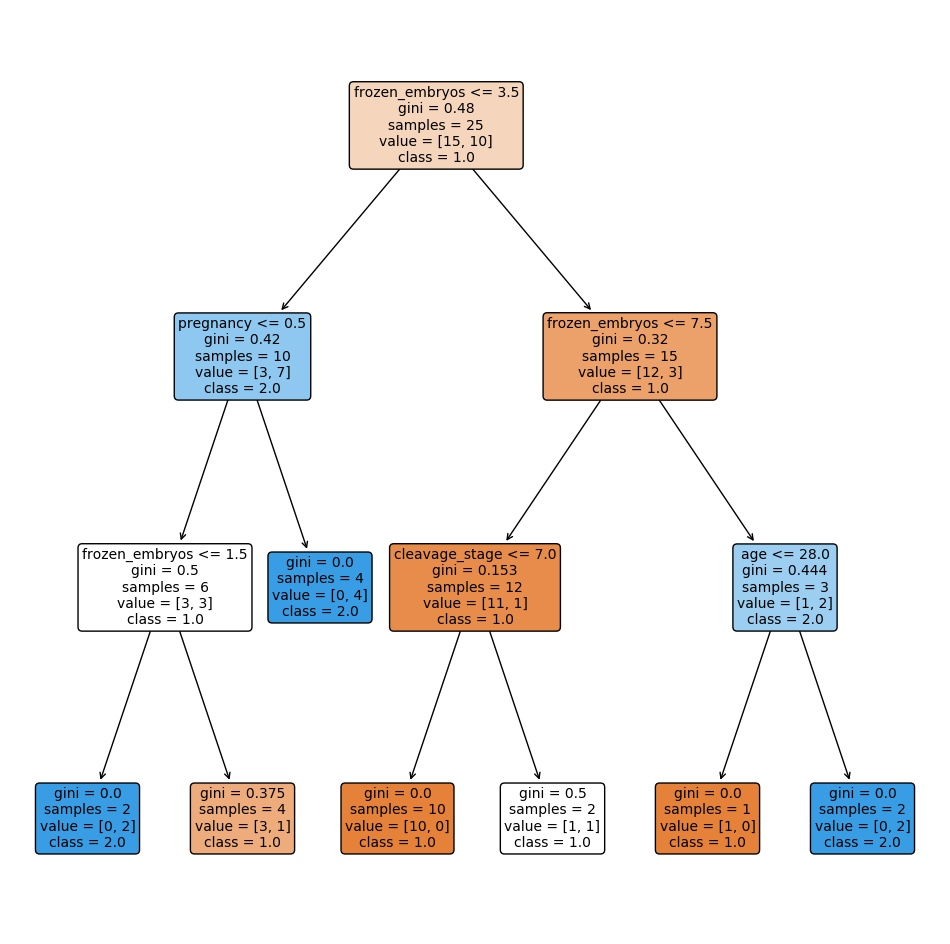
\includegraphics[width=\textwidth]{figures/ImageTreetree0.jpg}
\fcmfcaption{Drzewo decyzyjne CART dla pierwszego zbioru danych bez wariantu a3, indeks Gini jako miara podziału}\label{tree}
\end{figure}

\subsection{Losowy las}
\noindent Algorytm budowy losowego lasu \cite{randomForestPseudoCode} został przedstawiony w formie pseudokodu w Algorytmie~\ref{randomForest}. Działanie algorytmu opiera się na budowie z góry określonej liczby drzew, w taki sposób, że zbiorem treningowym dla każdego z~nich jest losowa próbka danych z oryginalnego zbioru treningowego. Sam proces budowy drzewa w stosunku do tradycyjnego algorytmu ulega nieznacznej modyfikacji -- zamiast szukać globalnie najlepszego podziału ustalamy losowy, mały zbiór kryteriów i dopiero z~niego wybieramy najlepszy podział, co znacząco ogranicza czas poszukiwania kryterium podziału.

\begin{algorithm}[H]
\caption{Pseudokod algorytmu losowego lasu}\label{randomForest}
\begin{algorithmic}
\Function{randomforest}{zbiór treningowy $X$, zbiór atrybutów $A$, liczba składowych drzew $B$}
\State $H \gets 0$
\For{$i \in 1,..,B$}
\State $X^{(i)} \gets $ niezależna próbka przykładów z $X$
\State $h_{i} \gets randomized\_tree\_learn(X^{(i),A)}$
\State $H \gets H \cup \{h_{i}\}$
\EndFor
\State return $H$
\EndFunction\\
\Function{randomized\_tree\_learn}{zbiór treningowy $X$, zbiór atrybutów $A$}
\For{każdego wierzchołka}
\State $a \gets $ mały podbiór zbioru $A$
\State dokonaj podziału na podstawie najlepszej, zgodnie z kryterium podziału, cechy w $a$
\EndFor
\State return zbudowane drzewo
\EndFunction
\end{algorithmic}
\end{algorithm}

Jeśli chodzi o dokonywanie klasyfikacji dla nowych przykładów, to proces jest realizowany w~następujących krokach:
\begin{enumerate}
    \item dla każdego drzewa znajdź rekomendowaną przez nie klasę dla przykładu,
    \item sprawdź, która z decyzji jest rekomendowana przez największą liczbę drzew,
    \item przypisz powyższą jako wynik klasyfikacji.
\end{enumerate}

\paragraph{Przykład z pierwszego zbioru danych}\mbox{}\\
Analogicznie jak dla przykładu dla CART dane uczące stanowią oryginalny zbiór z wyłączeniem wariantu a3, który posłuży do testów. Wizualizacja przykładu została zrealizowana z wykorzystaniem modelu RandomForestClassifier \cite{rfSklearn} również z biblioteki sklearn \cite{sklearn}. Wybrana została miara indeks Gini oraz ograniczenie do budowy zespołu składającego się z trzech drzew. Na Rysunkach \ref{rf1}, \ref{rf2} oraz \ref{rf3} zaprezentowane zostały kolejne estymatory wchodzące w skład modelu.

Pierwsze drzewo (patrz Rysunek \ref{rf1}) ma głębokość 4 i pozwala na klasyfikację przykładów do~klas 1 (w jednym liściu), 2 (w dwóch liściach) oraz 3 (w czterech liściach). Podział w korzeniu wykonywany jest na podstawie kryterium $infertility$, zaś pozostałe wykorzystane kryteria to $age$, $woman\_eval$ i $oocytes$. W fazie budowy drzewa pracowano na 29 przykładach ze zbioru danych. 

Drugi estymator (patrz Rysunek \ref{rf2}) ma głębokość 5 i zawiera 8 liści, z których 5 sugeruje przypisanie obiektom klasy 3, 2 -- klasy 2 i jeden klasy 4. Wiek kobiety jest kryterium podziału dokonywanego w korzeniu. Pozostałe użyte w tym drzewie kryteria to $develop\_quality$, $woman\_eval$, $oocytes$, $morpho\_quality$, $sperm$ oraz $infertility$, czyli wykorzystane zostały wszystkie dostępne atrybuty. Estymator został zbudowany na podstawie próbki 34 przykładów ze zbioru danych.

Ostatnie, trzecie, drzewo (patrz Rysunek \ref{rf3}) ma głębokość równą 5. Pozwala na klasyfikację przykładów do wszystkich możliwych klas, odpowiednio:
\begin{itemize}
    \item 4 liście sugerują przypisanie klasy 3,
    \item 3 liście sugerują przypisanie klasy 2,
    \item 1 liść sugeruje przypisanie klasy 4,
    \item 1 liść sugeruje przypisanie klasy 1.
\end{itemize}
Ten estymator dokonuje podziału w korzeniu na podstawie wartości na kryterium $morpho\_quality$, pozostałe użyte kryteria to: $infertility$, $sperm$, $oocytes$, $woman\_eval$ oraz $age$. Faza budowy drzewa zrealizowana została z wykorzystaniem 29 przykładów ze zbioru danych.

Patrząc na cały zespół, poszczególne estymatory wykorzystują różne kryteria podziału, co więcej -- tylko drugi wykorzystał każdy możliwy atrybut. Powstałe drzewa mają zbliżone głębokości. Każde z nich może sugerować przypisanie do innych zestawów klas, tylko ostatnie uwzględnia pełny wachlarz możliwości. Pierwsze drzewo jest najbardziej zbalansowanym klasyfikatorem. Drugie i~trzecie mają bardziej rozbudowane lewe poddrzewa (patrząc od korzenia).

Dla testowanego przykładu kolejne estymatory (patrz Rysunek \ref{rf1}, \ref{rf2} oraz \ref{rf3}) przydzielają następujące klasy:
\begin{itemize}
    \item estymator 1: klasa 2\\
    Otrzymana w wyniku przejścia do lewego wierzchołka $$age\leq35.0$$ następnie prawego $$woman\_eval\leq4.5$$ i lewego $$infertility\leq1.5$$ oraz na koniec do lewego liścia.
    \item estymator 2: klasa 3\\
    Jest wynikiem przejścia do prawego wierzchołka $$sperm\leq2.0$$ następnie prawego $$infertility\leq2.5$$ i lewego liścia.
    \item estymator 3: klasa 3\\
    Otrzymana na ścieżce do prawego wierzchołka $$woman\_eval\leq3.5$$ i następnie prawego liścia.
\end{itemize}
Ostatecznie predykcja klasy 3 została przypisana przez 2 z 3 drzew składowych, zatem wariant a3 ma przypisaną poprawną klasę 3.

\begin{figure}[H]
\centering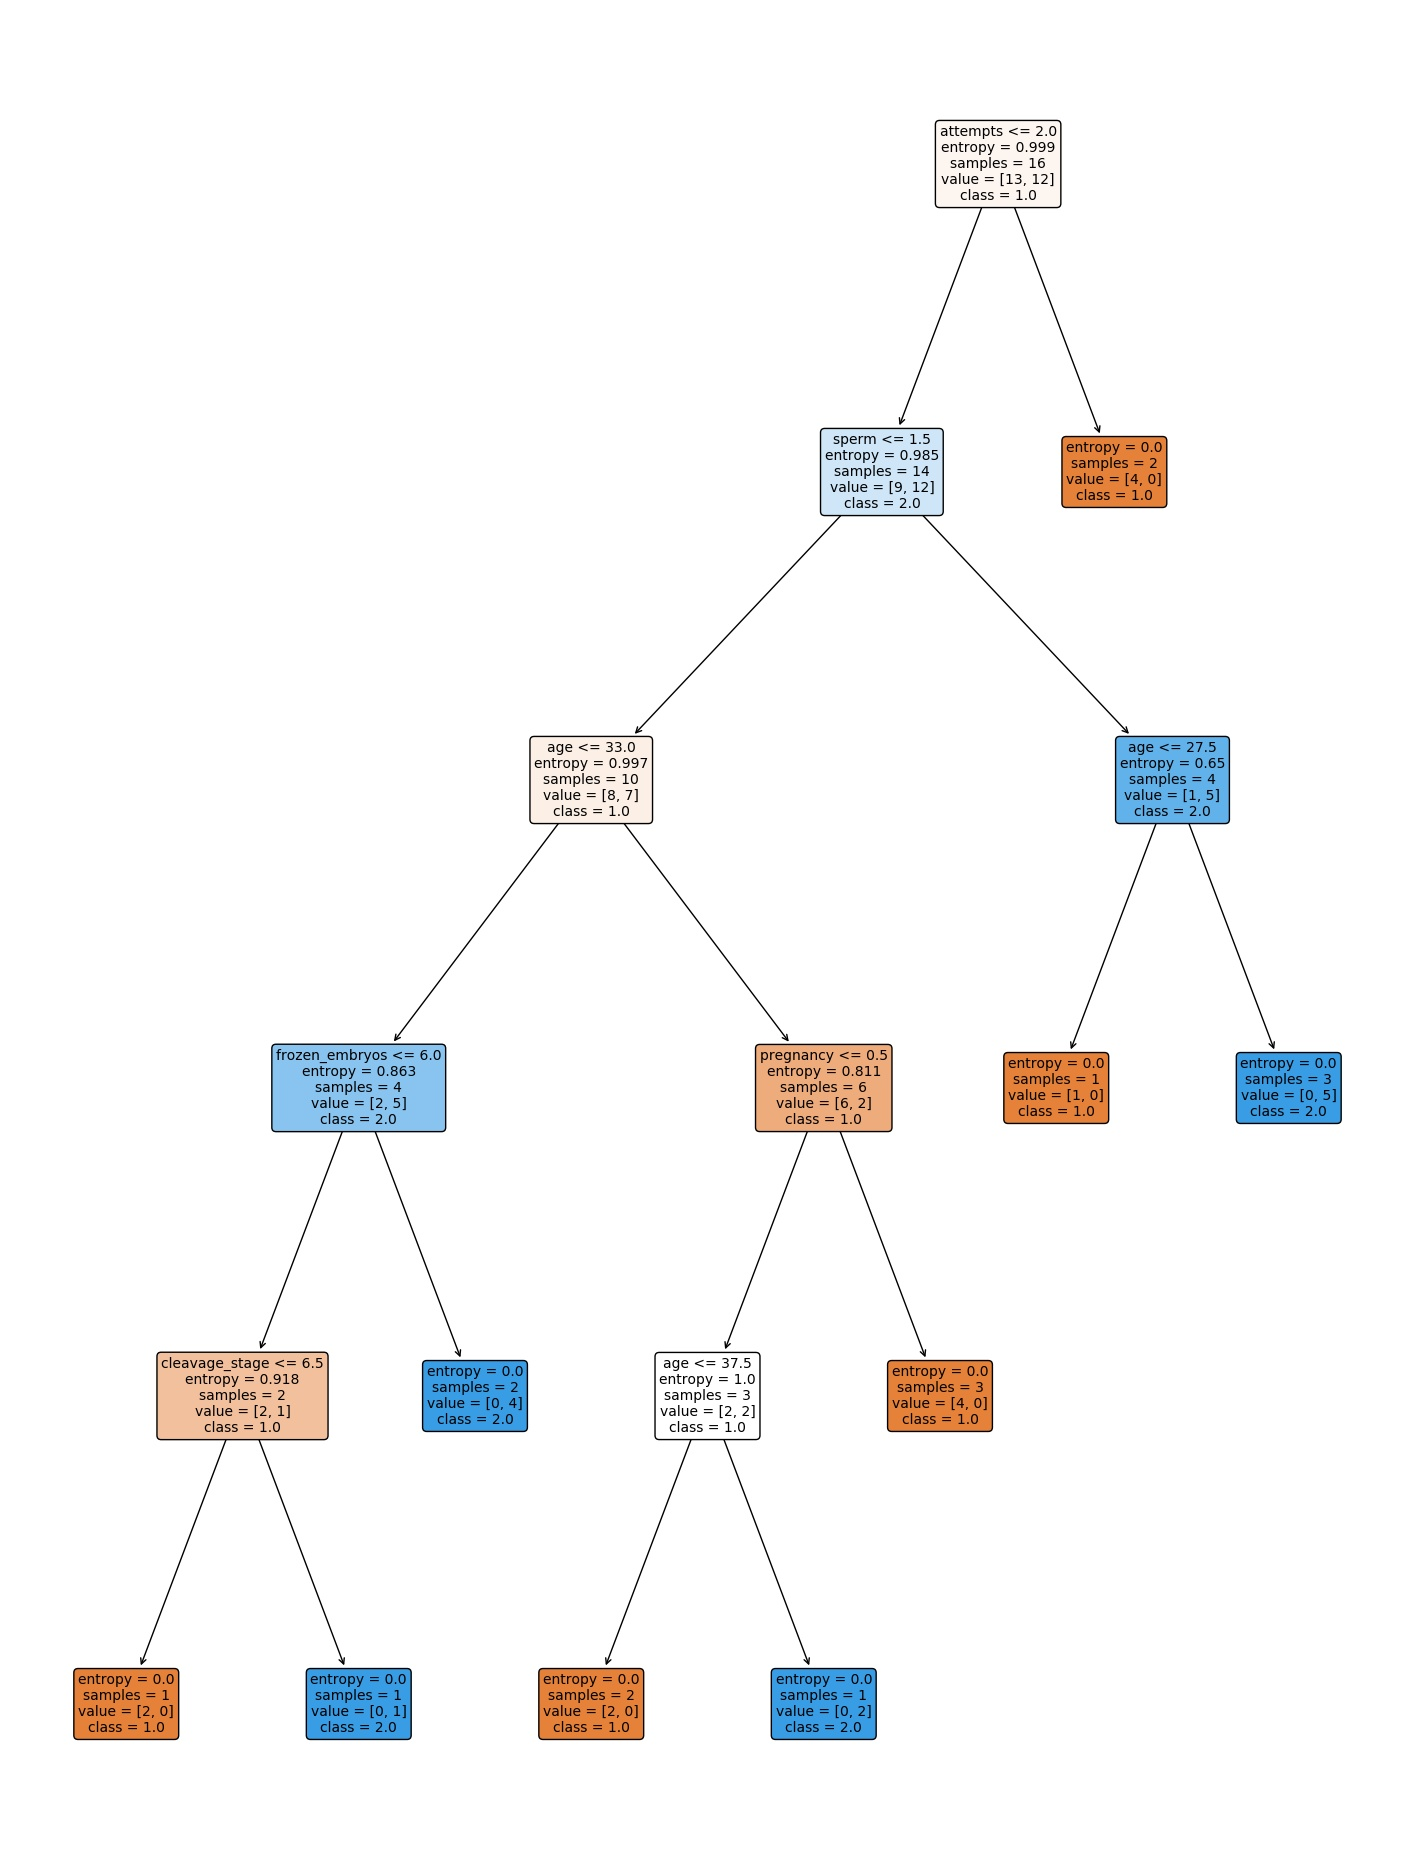
\includegraphics[width=\textwidth]{figures/ImageRFrandom_forest0_estimator_0.jpg}
\fcmfcaption{Losowy las - pierwsze drzewo dla zbioru pierwszego bez wariantu a3, indeks Gini jako miara podziału, 3 estymatory}\label{rf1}
\end{figure}
\begin{figure}[H]
\centering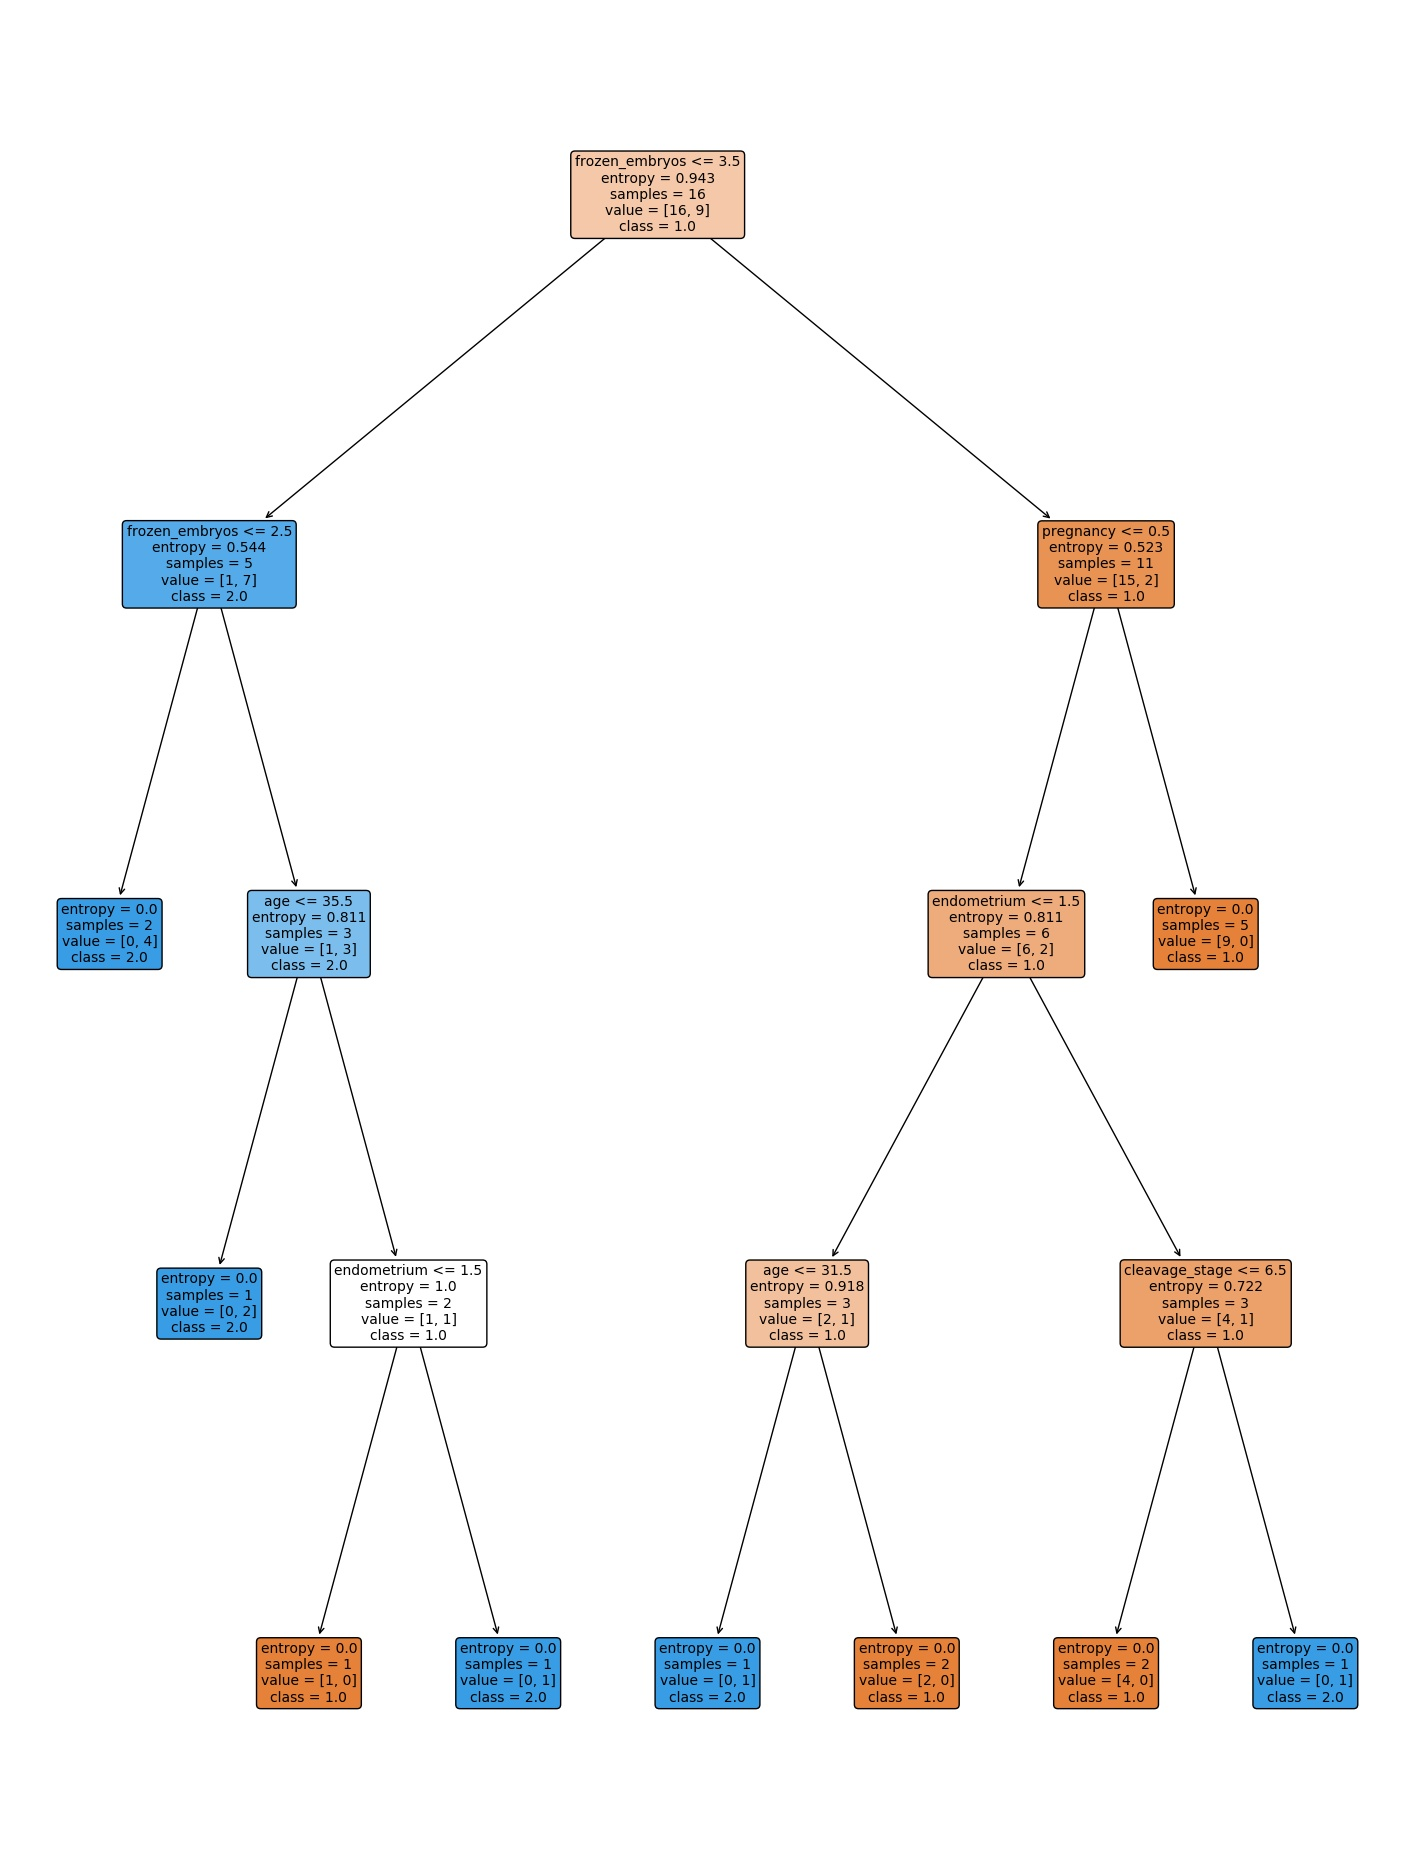
\includegraphics[width=\textwidth]{figures/ImageRFrandom_forest0_estimator_1.jpg}
\fcmfcaption{Losowy las - drugie drzewo dla zbioru pierwszego bez wariantu a3, indeks Gini jako miara podziału, 3 estymatory}\label{rf2}
\end{figure}
\begin{figure}[H]
\centering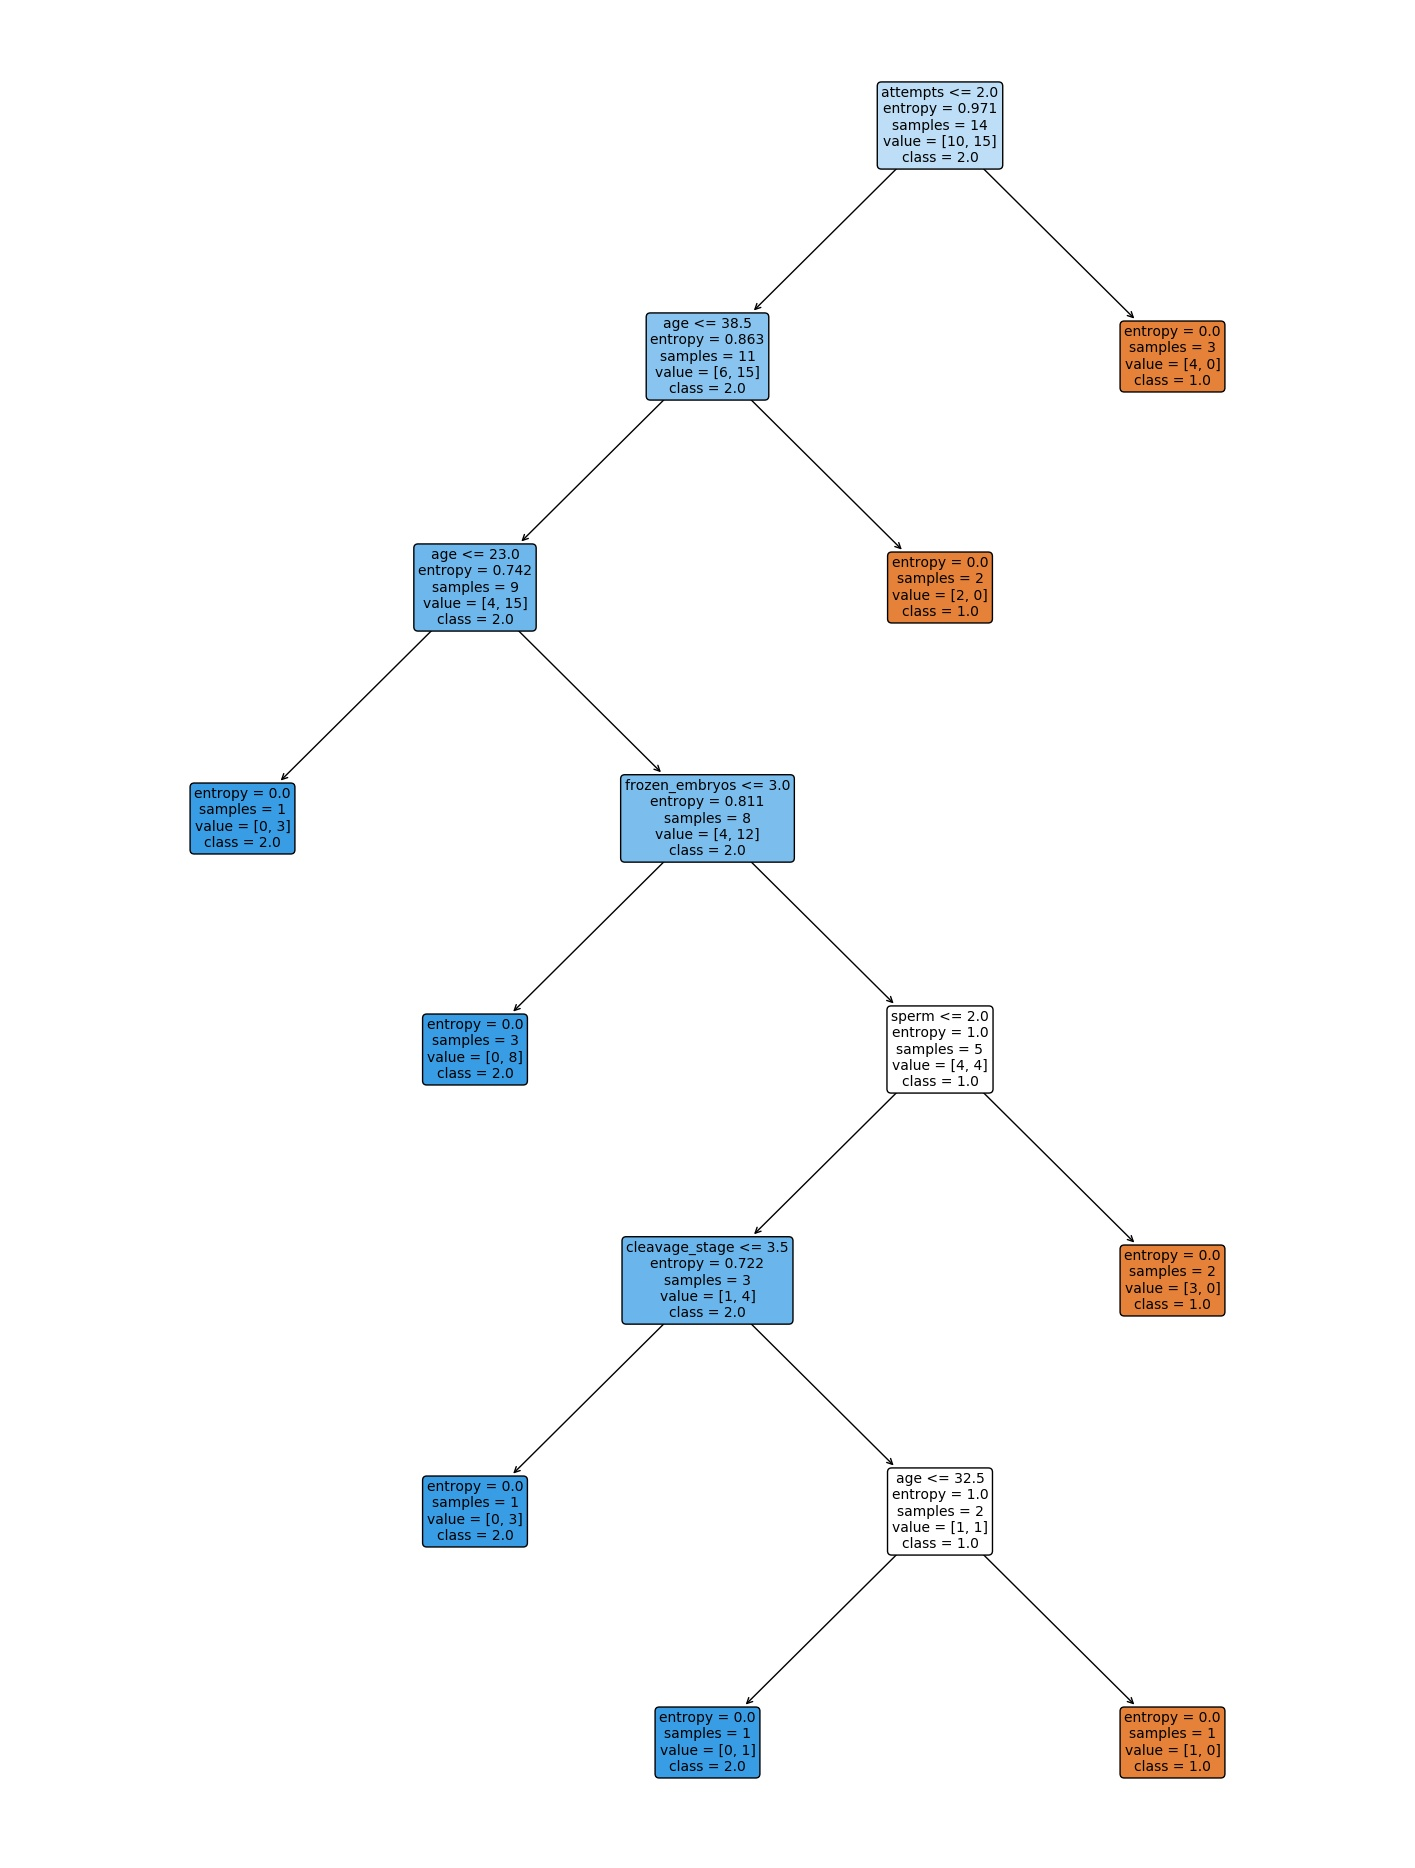
\includegraphics[width=\textwidth]{figures/ImageRFrandom_forest0_estimator_2.jpg}
\fcmfcaption{Losowy las - trzecie drzewo dla zbioru pierwszego bez wariantu a3, indeks Gini jako miara podziału, 3 estymatory}\label{rf3}
\end{figure}
\newpage


\chapter{Rezultaty}
\noindent Opisane w poprzednim rozdziale metody zostały wykorzystane do przygotowania kilku modeli. Modele drzew CART i losowy las były implementowane przy wykorzystaniu biblioteki sklearn \cite{sklearn}, zaś~pozostałe metody zaimplementowano samodzielnie przy wykorzystaniu języka Python. Repozytorium kodów źródłowych oraz pełne wyniki umieszczone są w załącznikach do pracy. Przetestowano następujące scenariusze eksperymentów:
\begin{itemize}
    \item wykorzystanie metody DRSA, algorytmu DOMLEM i prostego algorytmu klasyfikacji,
    \item wykorzystanie metody VC-DRSA, algorytmu DOMLEM i prostego algorytmu klasyfikacji,
    \item wykorzystanie metody DRSA, algorytmu DOMLEM i zaawansowanego algorytmu klasyfikacji,
    \item wykorzystanie metody VC-DRSA, algorytmu DOMLEM i zaawansowanego algorytmu klasyfikacji,
    \item wykorzystanie metody DRSA, algorytmu DOMApriori i prostego algorytmu klasyfikacji,
    \item wykorzystanie metody VC-DRSA, algorytmu DOMApriori i prostego algorytmu klasyfikacji,
    \item wykorzystanie metody DRSA, algorytmu DOMApriori i zaawansowanego algorytmu klasyfikacji,
    \item wykorzystanie metody VC-DRSA, algorytmu DOMApriori i zaawansowanego algorytmu klasyfikacji,
    \item wykorzystanie drzew CART,
    \item wykorzystanie losowego lasu.
\end{itemize}

Przy wykorzystaniu metody DRSA nie było potrzeby doboru wartości parametrów. Dla VC-DRSA należało dobrać wartość poziomu spójności -- testowane były liczby z przedziału od 0.05 do~0.95 włącznie, z krokiem co 0.05. Wartość 1 nie była testowana ze względu na fakt, iż dla~poziomu spójności równego 1 metoda VC-DRSA i DRSA otrzymują zawsze te same wyniki. Dodatkowo, testowanie odbywało się z krokiem co 0.05 dlatego, że zmiany w otrzymywanych wynikach dla tak małych zbiorów nie są znaczące dla małych zmian wartości parametru. W przypadku algorytmu DOMApriori koniecznym było ustalenie minimalnego wsparcia reguły i maksymalnej jej długości. Ostatecznie, wymagano wsparcia większego bądź równego 1 ze względu na fakt, iż dla większych wartości minimalnego wsparcia nie były pokrywane wszystkie obiekty. Maksymalną długość reguły ustalono na 3, gdyż dłuższe reguły pokrywały już tylko obiekty dotychczas pokryte oraz znacząco wpływały na wydłużenie czasu działania algorytmu. Dla DOMLEM oraz algorytmów klasyfikacji nie ustalano parametrów.

Dla drzew sprawdzano entropię i indeks Gini dla szukania najlepszego podziału oraz uwzględnianie bądź nie wagi klas w algorytmie -- tę możliwość stwarza implementacja algorytmu CART z~biblioteki sklearn. Natomiast dla losowego lasu, oprócz elementów wymienionych dla drzew, dobierano także liczbę estymatorów w zespole, wartość parametru $a$ określającego karę dla złożonych struktur w procedurze przycinania zbudowanych drzew oraz czy budując poszczególne estymatory dobierać niezależne próbki przykładów ze zbioru danych czy pracować na pełnym zbiorze.

Dla oceny poszczególnych modeli przeprowadzono walidacje krzyżową. Posłużono się metodą Leave-one-out \cite{articleLOO}, która polega na zbudowaniu tylu modeli ile obserwacji w zbiorze $n$, z których każdy uczony jest na $n-1$ wariantach, a testowany na jednym, niewykorzystanym do budowy modelu, przykładzie.

W Podrozdziałach 4.1 oraz~4.2 przestawione są ogólnie otrzymane wyniki wraz z dokładnym opisem rezultatów osiągniętych przez najlepsze zbudowane modele.

\section{Pierwszy zbiór danych}
\noindent W Tabeli \ref{res1} zebrano wartości trafności oraz miary F1-score dla najlepszych wersji, budowanych na~pierwszym zbiorze danych, modeli DRSA i VC-DRSA. Przy wykorzystaniu algorytmu DOMApriori minimalne wsparcie zostało ustalone na 1 a maksymalna długość reguły na 3.

Na podstawie Tabeli \ref{res1} modele DRSA osiągały trafność klasyfikacji z przedziału $0.59-0.76$. Wartość 0.76 osiągnięto dla~modelu korzystającego z algorytmu DOMApriori i zaawansowanej metody klasyfikacji. Oznacza ona, że średnia trafność dla 51 zbudowanych modeli -- przy wykorzystaniu walidacji metodą Leave-one-out -- plasuje się na poziomie nieco wyższym niż 75\%, około 3~na~4 modele dokonywały poprawnej klasyfikacji testowego wariantu. Można też zauważyć, że niewielki wpływ na wartość tej miary ma wybór algorytmu indukcji reguł decyzyjnych, zaś ważną role odgrywa metoda klasyfikacji -- dla zaawansowanego algorytmu rezultaty są istotnie lepsze (prosty algorytm klasyfikacji: $0.59-0.63$, zaawansowany: $0.75-0.76$, zatem trafność wyższa o~około 15\%).

Dla VC-DRSA osiągnięte wartości miary trafności były na zbliżonym poziomie ($0.75-0.78$) -- najsłabiej wypadła wersja z algorytmem DOMLEM i prostą metodą klasyfikacji. Eksperymenty walidacyjne pokazały, że takie modele klasyfikowały poprawnie średnio 75\% przykładów, czyli, w~odniesieniu do Leave-one-out, co czwarty zbudowany model przypisywał niepoprawną klasę testowemu przykładowi. Warto zauważyć, że w tym przypadku wybrany algorytm klasyfikacji nie~miał takiego znaczenia jak dla DRSA. Istotna była natomiast metoda indukcji reguł decyzyjnych -- dla algorytmu DOMLEM wysoka trafność była osiągana kosztem bardzo niskiej spójności -- nie jest to pożądane. Dopuszczenie dużej niespójności skutkuje powstaniem modelu zbyt uniwersalnego, za mało dopasowanego do problemu. 

W każdym z ujętych w Tabeli \ref{res1} modeli F1-score osiąga wartość 0, co podkreśla sygnalizowany wcześniej problem zbioru danych - występuje w nim zdecydowanie za mało przykładów dla dwóch z czterech klas decyzyjnych.

\begin{table}[H]
\caption{Wartości trafności i F1-score dla pierwszego zbioru danych - modele DRSA}\label{res1}
\centering
\begin{tabularx}{\textwidth}{llllllll}
\toprule Model & Algorytm ind. reguł & Algorytm klasyf. & Poziom spójności & Trafność & F1-score \\
\midrule
    DRSA & DOMLEM & prosty & - &  0.59 & 0.0\\\\
    VC-DRSA & DOMLEM & prosty & 0.45 & 0.75 & 0.0\\\\
    DRSA & DOMLEM & zaawansowany & - & 0.75 & 0.0\\\\
    VC-DRSA & DOMLEM & zaawansowany & 0.25 & 0.78 & 0.0\\\\
    DRSA & DOMApriori & prosty & - & 0.63 & 0.0\\\\
    VC-DRSA & DOMApriori & prosty & 0.9 & 0.78 & 0.0\\\\
    DRSA & DOMApriori & zaawansowany & - & 0.76 & 0.0\\\\
    VC-DRSA & DOMApriori & zaawansowany & 0.9 & 0.78 & 0.0\\\\
\bottomrule\end{tabularx}
\end{table}

Tabela \ref{res2} zawiera wartości trafności i miary F1-score dla modeli drzew i lasów. Przedstawione są także parametry poszczególnych wersji algorytmów. Dla wagi klas subbalans określanie wag klas przygotowywane jest na podstawie przykładów z próbki dla danego estymatora.

Wśród drzew CART najlepszy wynik osiągnięto nie stosując ważenia klas i korzystając z entropii jako miary do oceny podziału. Dla tej wersji 84\% wszystkich zbudowanych modeli poprawnie zaklasyfikowało testowy przykład. Ogółnie dla drzew CART trafność klasyfikacji mieści się w~przedziale $0.67-0.84$.

Najlepsze losowe lasy to te, które wykorzystywały entropię jako miarę podziału, nie wykorzystywały ważenia klas oraz składały się odpowiednio z 3 estymatorów. Osiągnęły one 86\% trafności klasyfikacji, co oznacza że spośród 51 modeli walidacyjnych 44 poprawnie zaklasyfikowały testowy przykład. Rozważane były także zespoły o większej liczbie drzew, jednak nie sprawdzały się one lepiej niż te zaraportowane w Tabeli \ref{res2}. Jeśli chodzi o ważenie klas dla tego zbioru najlepiej sprawdza się pominięcie go. Natomiast lepszą miarą oceny podziału okazała się w tym przypadku entropia -- średnio o 2\% wyższe wyniki niż dla indeksu Gini. Ogólnie trafność klasyfikacji dla losowych lasów mieściła się w przedziale $0.73-0.86$.

Miara F1-score osiąga, zarówno dla drzew CART jak i losowych lasów, zbliżone wartości do trafności klasyfikacji.

\begin{table}[H]
\caption{Wartości trafności i F1-score dla pierwszego zbioru danych - modele drzew}\label{res2}
\centering
\begin{tabularx}{\textwidth}{XXXXXX}
\toprule Model & Waga klas & Miara oceny podziału & Liczba estymatorów & Trafność & F1-score \\
\midrule
    drzewa CART & niestosowana & indeks Gini & - & 0.82 & 0.82\\\\
    drzewa CART & niestosowana & entropia & - & 0.84 & 0.84\\\\
    drzewa CART & zbalansowana & indeks Gini & - & 0.73 & 0.73\\\\
    drzewa CART & zbalansowana & entropia & - & 0.67 & 0.67\\\\
    losowy las & niestosowana & indeks Gini & 2 & 0.76 & 0.76\\\\
    losowy las & niestosowana & entropia & 2 & 0.78 & 0.78\\\\
    losowy las & zbalansowana & indeks Gini & 2 & 0.73 & 0.73\\\\
    losowy las & zbalansowana & entropia & 2 & 0.73 & 0.73\\\\
    losowy las & subbalans & indeks Gini & 2 & 0.73 & 0.73\\\\
    losowy las & subbalans & entropia & 2 & 0.73 & 0.73\\\\
    losowy las & niestosowana & indeks Gini & 3 & 0.78 & 0.78\\\\
    losowy las & niestosowana & entropia & 3 & 0.86 & 0.86\\\\
    losowy las & zbalansowana & indeks Gini & 3 & 0.76 & 0.76\\\\
    losowy las & zbalansowana & entropia & 3 & 0.82 & 0.82\\\\
    losowy las & subbalans & indeks Gini & 3 & 0.76 & 0.76\\\\
    losowy las & subbalans & entropia & 3 & 0.76 & 0.76\\\\
\bottomrule\end{tabularx}
\end{table}

Porównując modele DRSA i drzewiaste lepiej sprawdziły się te drugie, jednak różnice nie są tu znaczące, jeśli chodzi o wartości trafności. Dla miary F1-score zdecydowanie lepsze rezultaty osiągane są przez drzewa i lasy -- o około 70\%. Mimo problematycznego rozkładu obserwacji z poszczególnych klas, przygotowane modele osiągają dość wysoką wartość obu raportowanych miar.

Porównując DRSA i VC-DRSA można stwierdzić, iż wprowadzenie obniżonego poziomu spójności pozytywnie wpływa na skuteczność działania modelu, natomiast drzewa CART i losowy las dla tego zbioru danych sprawdzają się podobnie.

W Tabeli \ref{res3} zebrano dane na temat reguł wyindukowanych przez rozważane wersje metody DRSA - wartości długości, wsparcia, pokrycia i siły to dane uśrednione po zbiorze reguł dla~poszczególnych modeli.

Analizując dane w Tabeli \ref{res3} można zauważyć, że reguły indukowane przy wykorzystaniu algorytmu DOMLEM są średnio krótsze od tych, które zbudowane zostały z wykorzystaniem DOMApriori, co jest naturalną konsekwencją tego, jakie typy zbiorów reguł powstają przy wykorzystaniu tych metod. Ponadto dla DOMLEM powstałe reguły cechuje wyższe średnie wsparcie, pokrycie i siła -- co również jest następstwem indukcji minimalnego zbioru reguł w tym przypadku. Największą różnicę możemy zaobserwować w liczbie powstałych reguł -- dla DOMApriori jest ich kilkakrotnie więcej. 

\begin{table}[H]
\caption{Statystyki reguł dla pierwszego zbioru danych}\label{res3}
\centering
\begin{tabularx}{\textwidth}{Xllllll}
\toprule Model & Długość & Wsparcie & Pokrycie & Siła & Liczba reguł \\
\midrule
    DRSA, DOMLEM, prosty & 1.65 & 18.41 & 0.53 & 0.36 & 17\\\\
    VC-DRSA, DOMLEM, prosty, 0.45 & 1.1  & 24.1 & 0.87 & 0.47 & 10\\\\
    DRSA, DOMLEM, zaawansowany & 1.65 & 18.41 & 0.53 & 0.36 & 17\\\\
    VC-DRSA, DOMLEM, zaawansowany, 0.25 & 1.18 & 22.27 & 0.81 & 0.44 & 11\\\\
    DRSA, DOMApriori, prosty & 2.07 & 12.6 & 0.37 & 0.25 & 73\\\\
    VC-DRSA, DOMApriori, prosty, 0.9 & 2.25 & 23.57 & 0.59 & 0.46 & 186\\\\
    DRSA, DOMApriori, zaawansowany &  2.07 & 12.6 & 0.37 & 0.25 & 73\\\\
    VC-DRSA, DOMApriori, zaawansowany, 0.9 & 2.45 & 22.31 & 0.57 & 0.44 & 176\\\\
\bottomrule\end{tabularx}
\end{table}

Warto teraz dokładniej przyjrzeć się kilku najlepszym przygotowanym modelom. Dla metody DRSA wybrany został wariant dla algorytmu DOMLEM i złożonej metody klasyfikacji. Osiąga on trafność na poziomie 75\%. Jest to wynik bliski najlepszemu osiągniętemu dla tej metody. Taki wybór podyktowany jest zdecydowanie mniejszą liczbą reguł niż dla wersji korzystającej z~DOMApriori.
W Tabeli \ref{res4} przedstawiono reguły decyzyjne dla tego modelu. Nie pojawiły się wśród nich reguły opisujące obiekty należące do klasy \textit{co najmniej 4}. Wystąpiła jedna reguła opisująca warianty, dla których przypisana klasa to co najwyżej 1. Warunki często budowane są w oparciu o atrybut wieku kobiety, natomiast tylko jedna reguła wykorzystuje atrybut pochodzenie nasienia.  Kluczowymi atrybutami są niepłodność i oceny morfologiczna oraz rozwoju dla embrionów. Wśród wyindukowanych reguł pojawiło się 10 reguł składających się z jednego warunku. Warto też zauważyć, że najlepiej opisanymi uniami klas są: \textit{co najmniej klasa 3} oraz \textit{co najwyżej klasa~3}, co wynika z niezbalansowania obserwacji z poszczególnych klas w zbiorze - najwięcej obiektów ma~przypisaną klasę 3. Rozpatrując przykładową regułę: 
$$(age \leq  34.0) \wedge (morpho\_quality \geq  10.0) \implies (class \geq 3),$$ która kobietom mającym co najwyżej 34 lata i embrionom uzyskującym z punktu widzenia morfologicznego ocenę co najmniej 10 przypisuje klasę 3 lub 4, można zauważyć, że im młodsza jest pacjentka i im wyższa wartość oceny budowy embrionów tym przypisana zostaje lepsza klasa. Jest to zgodne z intuicją specjalistów.

\begin{table}[H]
\caption{Reguły wyindukowane dla metody DRSA przy wykorzystaniu algorytmu DOMLEM dla pierwszego zbioru danych}\label{res4}
    \centering
    \begin{tabularx}{\textwidth}{lX}
\toprule Oznaczenie & Reguła\\
\midrule
    Reguła 1 & $(age \geq  40.0) \wedge (woman\_eval \leq  2.0) \wedge (infertility \geq  3.0) \implies (class \leq 1)$\\ 
    Reguła 2 & $(age \geq  39.0) \wedge (infertility \geq  3.0) \implies (class \leq 2)$ \\
    Reguła 3 & $(morpho\_quality \leq  9.0) \wedge (age \geq  33.0) \wedge (infertility \geq  5.0) \implies (class \leq 2)$ \\
    Reguła 4 & $(develop\_quality \leq  4.0) \implies (class \leq 3)$\\ 
    Reguła 5 & $(infertility \geq  4.0) \implies (class \leq 3)$\\ 
    Reguła 6 & $(oocytes \geq  4.0) \implies (class \leq 3)$\\ 
    Reguła 7 & $(age \geq  35.0) \implies (class \leq 3)$ \\
    Reguła 8 & $(sperm \leq  2.0) \implies (class \leq 3)$ \\
    Reguła 9 & $(age \leq  34.0) \wedge (morpho\_quality \geq  10.0) \implies (class \geq 3)$ \\
    Reguła 10 & $(morpho\_quality \geq  15.0) \wedge (oocytes \leq  5.0) \implies (class \geq 3)$ \\
    Reguła 11 & $(age \leq  36.0) \wedge (infertility \leq  3.0) \wedge (oocytes \leq  5.0) \implies (class \geq 3)$\\
    Reguła 12 & $(age \leq  32.0) \implies (class \geq 3)$ \\
    Reguła 13 & $(infertility \leq  1.0) \wedge (develop\_quality \geq  4.0) \implies (class \geq 3)$ \\
    Reguła 14 & $(infertility \leq  2.0) \wedge (oocytes \leq  5.0) \implies (class \geq 3)$ \\
    Reguła 15 & $(age \leq  39.0) \implies (class \geq 2)$\\ 
    Reguła 16 & $(woman\_eval \geq  3.0) \implies (class \geq 2)$\\ 
    Reguła 17 & $(infertility \leq  2.0) \implies (class \geq 2)$\\
\bottomrule\end{tabularx}
\end{table}

Spośród modeli VC-DRSA do dalszej analizy, mimo niskiego poziomu spójności ($l=0.25$), weźmy wersję dla DOMLEM i zaawansowanego algorytmu klasyfikacji. Taki wybór podyktowany jest zdecydowanie mniejszą liczbą reguł, niż dla pozostałych, równie dobrych jeśli chodzi o wartość trafności, wariantów. Zbiór reguł dla tej wersji, ujęty w Tabeli \ref{res5}, podobnie jak poprzedni, nie zawiera reguł opisujących przypisanie do klasy \textit{co najmniej 4}, a dominują w nim reguły dotyczące przybliżeń klasy 2 i 3, co odzwierciedla liczbę obiektów z poszczególnych klas w danych wejściowych. Warunki w regułach najczęściej dotyczą wieku kobiety -- im jest ona młodsza tym proponowane są przypisania do lepszych klas. Dla 9 reguł pojawia się pojedynczy warunek, tylko~2 składają się z koniunkcji dwóch warunków, co związane jest z obniżonym poziomem spójności. Analizując przykładową regułę: $$(age \geq  40.0) \wedge (woman\_eval \leq  2.0) \implies (class \leq 1),$$ która kobietom w wieku 40 lat lub starszym i uzyskującym w ocenie specjalisty notę nie większą niż 2 przypisuje klasę 1, możemy zauważyć, że pacjentki starsze, słabo ocenione przez ginekologów czy położników klasyfikowane są do najsłabszej z rozważanych klas. Jest to zgodne z intuicyjnym rozważaniem. Warto też zauważyć, że w zbiorze reguł najmniej warunków dotyczy oceny embrionu - jest to różnica w stosunku do poprzedniego przykładu. Prawdopodobnie wynika ona z niskiego poziomu spójności, skutkującego także małą liczbą reguł w minimalnym zbiorze.

\begin{table}[H]
\caption{Reguły wyindukowane dla metody VC-DRSA, $l=0.25$ przy wykorzystaniu algorytmu DOMLEM dla pierwszego zbioru danych}\label{res5}
    \centering
    \begin{tabularx}{\textwidth}{lX}
\toprule Oznaczenie & Reguła\\
\midrule
    Reguła 1 & $(age \geq  40.0) \wedge (woman\_eval \leq  2.0) \implies (class \leq 1)$\\ 
    Reguła 2 & $(age \geq  38.0) \implies (class \leq 2) $\\
    Reguła 3 & $(oocytes \geq  6.0) \wedge (age \geq  36.0) \implies (class \leq 2) $\\
    Reguła 4 & $(morpho\_quality \leq  9.0) \implies (class \leq 2) $\\
    Reguła 5 & $(age \geq  27.0) \implies (class \leq 3) $\\
    Reguła 6 & $(sperm \leq  2.0) \implies (class \leq 3) $\\
    Reguła 7 & $(age \leq  38.0) \implies (class \geq 3) $\\
    Reguła 8 & $(infertility \leq  2.0) \implies (class \geq 3) $\\
    Reguła 9 & $(age \leq  39.0) \implies (class \geq 2) $\\
    Reguła 10 & $(woman\_eval \geq  3.0) \implies (class \geq 2) $\\
    Reguła 11 & $(infertility \leq  2.0) \implies (class \geq 2)$ \\
\bottomrule\end{tabularx}
\end{table}

Najlepszym zbudowanym drzewem CART jest dla tego zbioru wariant niewykorzystujący wagi klas i stosujący entropię jako miarę oceny podziału (Rysunek \ref{res6}).

W drzewie (Rysunek \ref{res6}) są 4 liście, z których 3 sugerują przypisanie obiektom klasy 3. Pozostały liść dotyczy klasy 2. Pierwszy podział dokonany jest za względu na wiek kobiety, co~podkreśla istotność tego kryterium w procesie decyzyjnym. Kolejne dwa alternatywne podziały różnicują warianty ze względu na wartości na kryteriach oceniających odpowiednio liczbę oocytów i niepłodność kobiety. Warto też zauważyć, że drzewo mogłoby zostać uproszczone, gdyż kobietom mającym mniej niż 38 lat, niezależnie od kolejnej decyzji, zostanie przypisana klasa 3. Zaletą zbudowanego klasyfikatora jest niewątpliwie jego niska złożoność - jego głębokość wynosi 2.

\begin{figure}[H]
\centering\includegraphics[width=\textwidth]{figures/ImageTreetree1_final.jpg}
\fcmfcaption{Najlepsze zbudowane drzewo CART, entropia jako miara oceny podziału, dla pierwszego zbioru danych}\label{res6}
\end{figure}
\newpage
Wśród modeli lasów opisany zostanie wariant niestosujący wag klas, składający się z 3 drzew i aplikujący entropię do oceny podziału. Na Rysunkach \ref{res7}, \ref{res8} oraz \ref{res9}. zostały przedstawione drzewa wchodzące w skład zespołu.

Pierwszy z estymatorów (Rysunek \ref{res7}) pracuje na 32 obiektach zbioru danych. Występuje w~nim 8 liści, z których 6 sugeruje przypisanie obiektom klasy 3 oraz po jednym odpowiednio klas 1 i 2. Podziały dokonywane są w oparciu o atrybuty dotyczące ogólnej oceny kobiety przez specjalistę, pochodzenia spermy i oceny rozwoju embrionów. Jest to ciekawa losowa próbka kryteriów, gdyż dla wcześniej zaprezentowanych modeli nie były one istotne. Dodatkowo, zaproponowane drzewo możnaby uprościć: w wierzchołkach $sperm \leq 2$ oraz $woman\_eval \leq 3.5$ zarówno lewy jak~i~prawy liść przypisuje obiektom klasę 3. Zredukowałoby to także liczbę wykorzystanych kryteriów o atrybut podziału dotyczący pochodzenia spermy. Powstałe drzewo ma głębokość 3, jest więc bardziej złożone niż najlepszy wariant dla drzew CART (Rysunek \ref{res6}).

Drugi estymator (Rysunek \ref{res8}) zawiera 6 liści, 3 z nich sugerują przypisanie klasy 3, a pozostałe -- klasy 2. Drzewo zbudowane zostało na podstawie 35 przykładów ze zbioru. Wykorzystane kryteria opisują ocenę kobiety przez specjalistę, pochodzenie spermy, morfologiczną ocenę embrionów i wiek kobiety. Najistotniejszy podział dokonany jest, jak dla poprzedniego estymatora (Rysunek~\ref{res7}.), na podstawie oceny kobiety przez specjalistę. Zbudowane drzewo również można uprościć: w wierzchołku $morpho\_quality \leq 13.5$ zarówno w lewym jak i prawym liściu obiektom przypisywana jest klasa 3.

Ostatni, trzeci, estymator (Rysunek \ref{res9}) pracuje na 34 obiektach. Składa się z 5 liści, z których 3 sugerują przypisanie klasy 3, a pozostałe -- klasy 2. Użyte kryteria opisują pochodzenie spermy, morfologiczną i rozwojową ocenę embrionów oraz niepłodność pary. Zaproponowane drzewo mogłoby zostać uproszczone - w wierzchołku $develop\_quality \leq 3.5$ oba liście przypisują obiektom klasę 3. Głębokość drzewa jest taka sama jak w przypadku pozostałych estymatorów w zespole -- wynosi 3.

Cały zespół (Rysunki \ref{res7}, \ref{res8} oraz \ref{res9}) stanowi dość rozbudowaną i ciekawą propozycję klasyfikatora uwzględniającego wiele kryteriów. Pozwala na klasyfikowanie obiektów do trzech spośród 4 możliwych klas decyzyjnych. 

\begin{figure}[H]
\centering\includegraphics[width=\textwidth]{figures/ImageRFrandom_forest1_estimator_0_final.jpg}
\fcmfcaption{Najlepszy zbudowany losowy las dla pierwszego zbioru danych, stosujący entropię jako miarę oceny podziału -- pierwszy estymator}\label{res7}
\end{figure}
\begin{figure}[H]
\centering\includegraphics[width=\textwidth]{figures/ImageRFrandom_forest1_estimator_1_final.jpg}
\fcmfcaption{Najlepszy zbudowany losowy las dla pierwszego zbioru danych, stosujący entropię jako miarę oceny podziału -- drugi estymator}\label{res8}
\end{figure}
\begin{figure}[H]
\centering\includegraphics[width=\textwidth]{figures/ImageRFrandom_forest1_estimator_2_final.jpg}
\fcmfcaption{Najlepszy zbudowany losowy las dla pierwszego zbioru danych, stosujący entropię jako miarę oceny podziału -- trzeci estymator}\label{res9}
\end{figure}
\newpage
\section{Drugi zbiór danych}
\noindent W Tabeli \ref{res1-2017} zebrano wartości trafności oraz miary F1-score dla najlepszych wersji, budowanych na~drugim zbiorze danych, modeli DRSA i VC-DRSA. Przy wykorzystaniu algorytmu DOMApriori, analogicznie jak dla poprzedniego zbioru, minimalne wsparcie zostało ustalone na 1 a maksymalna długość reguły na 3.

Wśród modeli DRSA (Tabela \ref{res1-2017}) najlepiej sprawdził się ten, w którym wykorzystano algorytm DOMApriori i zaawansowaną metodę klasyfikacji. Uzyskał 40-procentową trafność w eksperymentach walidacyjnych, jest ona jednak dość niska. Ogólnie wartości trafności dla metody DRSA mieściły się dla tego zbioru w przedziale $0.36-0.4$. Biorąc pod uwagę F1-score, najlepiej sprawdził się algorytm DOMLEM i prosta metoda klasyfikacji. Uzyskał wartość 0.48.

Dla VC-DRSA (Tabela \ref{res1-2017}) najwyższy wynik osiągnięty został dla zaawansowanego algorytmu klasyfikacji -- 0.4. Wybór algorytmu indukcji reguł decyzyjnych nie wpływał na wartość trafności w tym przypadku, natomiast dla DOMLEM zanotowane zostały większe wartości F1-score (0.48 i~0.5). Trafność, podobnie jak dla DRSA jest niska, mieści się w przedziale $0.36-0.4$. Patrząc na~F1-score, najlepszy model VC-DRSA korzystał z algorytmu DOMLEM i zaawansowanej metody klasyfikacji.

Porównując wyniki dla VC-DRSA i DRSA są one, zarówno jeśli chodzi o trafność jak i F1-score na zbliżonym poziomie. Dla tego zbioru obie metody uzyskały dość słabe rezultaty.

\begin{table}[H]
\caption{Wartości trafności i F1-score dla drugiego zbioru danych - modele DRSA}\label{res1-2017}
\centering
\begin{tabularx}{\textwidth}{llllllll}
\toprule Model & Algorytm ind. reguł & Algorytm klasyf. & Poziom spójności & Trafność & F1-score \\
\midrule
    DRSA & DOMLEM & prosty & - & 0.36 & 0.48\\\\
    VC-DRSA & DOMLEM & prosty & 0.9 & 0.36 & 0.48 \\\\
    DRSA & DOMLEM & zaawansowany & - & 0.36 & 0.45 \\\\
    VC-DRSA & DOMLEM & zaawansowany & 0.8 & 0.4 & 0.5\\\\
    DRSA & DOMApriori & prosty & - & 0.36 & 0.45 \\\\
    VC-DRSA & DOMApriori & prosty & 0.9 & 0.36 & 0.45\\\\
    DRSA & DOMApriori & zaawansowany & - & 0.4 & 0.46 \\\\
    VC-DRSA & DOMApriori & zaawansowany & 0.9 & 0.4 & 0.46\\\\
\bottomrule\end{tabularx}
\end{table}

W Tabeli \ref{res2-2017} zawarte są wartości trafności i miary F1-score dla modeli drzew i lasów. Przedstawione są także parametry poszczególnych wersji algorytmów. Dla wagi klas subbalans określanie wag klas przygotowywane jest na podstawie przykładów z próbki dla danego estymatora.

Jeśli chodzi o drzewa CART, nie jest tu obserwowalna różnica w wartościach trafności i F1-score raportowanych w Tabeli \ref{res2-2017}. Co więcej, wartości dla obu miar są takie same i wynoszą 0.56.

Dla losowych lasów (Tabela \ref{res2-2017}) lepsze rezultaty osiągane są przez modele składające się z~większej liczby estymatorów. Mieszczą się one w przedziale $0.68-0.76$. Ponadto dla lasów składających się z dwóch drzew lepszą miarą oceny podziału okazała się entropia (zysk około 4\%), natomiast dla tych z trzech -- indeks Gini (zysk około 4\%). Dla większej niż 3 liczby estymatorów w zespole nie był obserwowany wzrost wartości żadnej z raportowanych miar stąd dane te nie są zawarte w Tabeli \ref{res2-2017}.

Losowe lasy sprawdziły się znacząco lepiej niż drzewa CART. może być to związane z faktem wykorzystania w zespole kilku drzew, pracujących na różnych próbkach danych i kryteriach.

\begin{table}[H]
\caption{Wartości trafności i F1-score dla drugiego zbioru danych - modele drzew}\label{res2-2017}
\centering
\begin{tabularx}{\textwidth}{XXXXXX}
\toprule Model & Waga klas & Miara oceny podziału & Liczba estymatorów & Trafność & F1-score \\
\midrule
    drzewa CART & niestosowana & indeks Gini & - & 0.56 & 0.56\\\\
    drzewa CART & niestosowana & entropia & - & 0.56 & 0.56\\\\
    drzewa CART & zbalansowana & indeks Gini & - & 0.56 & 0.56\\\\
    drzewa CART & zbalansowana & entropia & - & 0.56 & 0.56\\\\
    losowy las & niestosowana & indeks Gini & 2 & 0.68 & 0.68\\\\
    losowy las & niestosowana & entropia & 2 & 0.76 & 0.76\\\\
    losowy las & zbalansowana & indeks Gini & 2 & 0.64 & 0.64\\\\
    losowy las & zbalansowana & entropia & 2 & 0.64 & 0.64\\\\
    losowy las & subbalans & indeks Gini & 2 & 0.68 & 0.68\\\\
    losowy las & subbalans & entropia & 2 & 0.76 & 0.76\\\\
    losowy las & niestosowana & indeks Gini & 3 & 0.76 & 0.76\\\\
    losowy las & niestosowana & entropia & 3 &  0.76 & 0.76\\\\
    losowy las & zbalansowana & indeks Gini & 3 & 0.72 & 0.72\\\\
    losowy las & zbalansowana & entropia & 3 & 0.68 & 0.68\\\\
    losowy las & subbalans & indeks Gini & 3 & 0.76 & 0.76\\\\
    losowy las & subbalans & entropia & 3 & 0.68 & 0.68\\\\
\bottomrule\end{tabularx}
\end{table}

Porównując wyniki dla metod DRSA i drzew zdecydowanie lepiej sprawdziły się te drugie -- tu~uzyskane rezultaty są dość wysokie i sięgają nawet 76\% zarówno dla trafności jak i F1-score.
\newpage
Tabela \ref{res3-2017} zawiera dane na temat reguł wyindukowanych przez poszczególne warianty metody DRSA -- wartości długości, wsparcia, pokrycia i siły to dane uśrednione po zbiorze reguł dla~poszczególnych modeli.

Z danych w Tabeli \ref{res3-2017} można wyciągnąć wniosek, że indukowane reguły miały średnio dwa warunki. Ponadto im mniejsza jest wartość średniej długości reguł, tym większe jest średnie wsparcie, pokrycie oraz siła. Wykorzystanie algorytmu DOMApriori skutkowało powstaniem większych zbirów reguł, co bezpośrednio wynika z faktu, że indukuje on satysfakcjonujący, a nie minimalny -- jak~DOMLEM, zbiór reguł. Poszczególne modele budują reguły wspierane przez średnio dwa obiekty. Pokrywa to od 25 do 45\% wariantów z poszczególnych przybliżeń. Ze względu na mniejszą liczbę reguł faworyzowane może być podejście DOMLEM, wpływa to na czytelność i interpretowalność modelu.

\begin{table}[H]
\caption{Statystyki reguł dla drugiego zbioru danych}\label{res3-2017}
\centering
\begin{tabularx}{\textwidth}{Xllllll}
\toprule Model & Długość & Wsparcie & Pokrycie & Siła & Liczba reguł \\
\midrule
    DRSA, DOMLEM, prosty & 1.86 & 2.29 & 0.32 & 0.09 & 7\\\\
    VC-DRSA, DOMLEM, prosty, 0.45 &  1.86 & 2.29 & 0.32 & 0.09 & 7\\\\
    DRSA, DOMLEM, zaawansowany & 1.86 & 2.29 & 0.32 & 0.09 & 7\\\\
    VC-DRSA, DOMLEM, zaawansowany, 0.25 & 1.83 & 3.5 & 0.45 & 0.14 & 6\\\\
    DRSA, DOMApriori, prosty & 2.21 & 1.74 & 0.25 & 0.07 & 19\\\\
    VC-DRSA, DOMApriori, prosty, 0.9 &  2.21 & 1.74 & 0.25 & 0.07 & 19\\\\
    DRSA, DOMApriori, zaawansowany & 2.21 & 1.74 & 0.25 & 0.07 & 19\\\\
    VC-DRSA, DOMApriori, zaawansowany, 0.9 & 2.21 & 1.74  & 0.25 & 0.07 & 19 \\\\
\bottomrule\end{tabularx}
\end{table}

Przyglądając się dokładniej kilku najlepszym przygotowanym modelom i rozpoczynając od metody DRSA, wybrana została wersja korzystająca z algorytmu DOMApriori oraz zaawansowanego algorytmu klasyfikacji. Co istotne, mimo generacji satysfakcjonującego, a nie minimalnego zbioru reguł dysponujemy 19 regułami, co bezpośrednio wynika z wielkości zbioru danych. W Tabeli \ref{res4-2017} zostały przedstawione przygotowane reguły.

Spośród reguł przedstawionych w Tabeli \ref{res4-2017} 9 stanowią konstrukcje o dwuelementowej części warunkowej, 7 o trójelementowej, zaś pozostałe 3 to jednoelementowe wersje. W aż 11 regułach wykorzystany jest warunek na kryterium wieku kobiety, co świadczy o istotności tego elementu. Zbiór reguł pokrywa tylko dwa typy przybliżeń unii klas: \textit{co najwyżej klasa 1} i \textit{co najmniej klasa~2}, gdyż w przykładach w zbiorze występują tylko te dwie z czterech możliwych klas decyzyjnych. Weźmy przykładową regułę: $$(age \leq  31.0) \wedge (attempts \leq  1.0) \wedge (sperm \leq  2.0) \implies (class \geq 2)$$ która kobietom w wieku 31 lat lub poniżej, od których pozyskano 1 lub 2 oocyty i liczba nieudanych transferów embrionów nie przekracza 3 oraz przy wykorzystaniu spermy o koncentracji plemników w preparacie powyżej 5 milionów przypisuje klasę 2 lub wyższą. Dla takiego sformułowania do~lepszych klas przypisywane są pary młodsze, mające niewiele nieudanych prób transferu embrionów i dysponujące spermą o wysokiej koncentracji plemników, co jest zgodne z intuicją.

\begin{table}[H]
\caption{Reguły wyindukowane dla metody DRSA przy wykorzystaniu algorytmu DOMLEM dla drugiego zbioru danych}\label{res4-2017}
    \centering
    \begin{tabularx}{\textwidth}{lX}
\toprule Oznaczenie & Reguła\\
\midrule
    Reguła 1 & $(age \geq  42.0) \implies (class \leq 1)$\\ 
    Reguła 2 & $(sperm \geq  3.0) \implies (class \leq 1)$\\ 
    Reguła 3 & $(pregnancy \leq  0.0) \wedge (attempts \geq  3.0) \implies (class \leq 1)$\\ 
    Reguła 4 & $(pregnancy \leq  0.0) \wedge (sperm \geq  2.0) \implies (class \leq 1)$\\ 
    Reguła 5 & $(attempts \geq  3.0) \wedge (frozen\_embryos \leq  2.0) \implies (class \leq 1)$\\ 
    Reguła 6 & $(attempts \geq  3.0) \wedge (sperm \geq  2.0) \implies (class \leq 1)$\\ 
    Reguła 7 & $(endometrium \geq  2.0) \wedge (sperm \geq  2.0) \implies (class \leq 1)$\\ 
    Reguła 8 & $(sperm \geq  2.0) \wedge (cleavage\_stage \geq  8.0) \implies (class \leq 1)$\\ 
    Reguła 9 & $(age \geq  40.0) \wedge (pregnancy \leq  0.0) \implies (class \leq 1)$\\ 
    Reguła 10 & $(age \geq  40.0) \wedge (frozen\_embryos \leq  2.0) \implies (class \leq 1)$\\ 
    Reguła 11 & $(age \geq  23.0) \wedge (frozen\_embryos \leq  2.0) \wedge (cleavage\_stage \geq  8.0) \implies (class \leq 1)$\\ 
    Reguła 12 & $(age \geq  33.0) \wedge (pregnancy \leq  0.0) \wedge (cleavage\_stage \geq  8.0) \implies (class \leq 1)$\\ 
    Reguła 13 & $(age \leq  22.0) \implies (class \geq 2)$\\ 
    Reguła 14 & $(sperm \leq  2.0) \wedge (frozen\_embryos \geq  8.0) \implies (class \geq 2)$\\ 
    Reguła 15 & $(age \leq  32.0) \wedge (pregnancy \geq  1.0) \wedge (endometrium \leq  1.0) \implies (class \geq 2)$\\ 
    Reguła 16 & $(age \leq  32.0) \wedge (pregnancy \geq  1.0) \wedge (sperm \leq  2.0) \implies (class \geq 2)$\\ 
    Reguła 17 & $(age \leq  32.0) \wedge (sperm \leq  2.0) \wedge (cleavage\_stage \leq  2.0) \implies (class \geq 2)$\\ 
    Reguła 18 & $(age \leq  31.0) \wedge (attempts \leq  1.0) \wedge (endometrium \leq  1.0) \implies (class \geq 2)$\\ 
    Reguła 19 & $(age \leq  31.0) \wedge (attempts \leq  1.0) \wedge (sperm \leq  2.0) \implies (class \geq 2)$\\
\bottomrule\end{tabularx}
\end{table}

Wśród modeli VC-DRSA najlepiej sprawdziła się wersja korzystająca a algorytmu DOMApriori i zaawansowanej metody klasyfikacji. Jednak, z uwagi na wysoki poziom spójności ($l=0.9$), wersja ta nie różni się od poprzednio opisanej i nie wymaga dodatkowego komentarza.

Dla drzew CART do opisu wybrana została wersja niestosująca ważenia klas oraz wykorzystująca indeks Gini jako miarę do oceny podziału. Zbudowane w tym przypadku drzewo zostało przedstawione na Rysunku \ref{res6-2017}.

Drzewo (Rysunek \ref{res6-2017}) składa się z 9 liści, z których 5 sugeruje przypisanie obiektom klasy~2, zaś~pozostałe 4 -- klasy 1. Główny podział wykonywany jest na podstawie kryterium mówiącego o liczbie zamrożonych embrionów. Pozostałe wykorzystane kryteria dotyczą informacji czy parze udało się dotychczas osiągnąć ciążę, oceny morfologicznej rozwoju embrionu oraz jakości i pochodzenia spermy. Zbudowane drzewo ma głębokość 4, ma więc dość złożoną strukturę.

\begin{figure}[H]
\centering\includegraphics[width=\textwidth]{figures/ImageTreetree0_final.jpg}
\fcmfcaption{Najlepsze zbudowane drzewo CART dla zbioru drugiego, indeks Gini jako miara oceny podziału}\label{res6-2017}
\end{figure}

\newpage
Spośród losowych lasów opisany zostanie wariant składający się z 3 estymatorów, nie stosujący wag klas oraz wykorzystujący entropię jako miarę oceny podziału. Poszczególne estymatory należące do zespołu zostały przedstawione na Rysunkach \ref{res7-2017}, \ref{res8-2017} oraz \ref{res9-2017}.

Pierwszy estymator (Rysunek \ref{res7-2017}) zawiera 9 liści, z których 5 sugeruje przypisanie obiektowi klasy 1, a pozostałe 4 -- klasy 2. Do zbudowania drzewa wykorzystanych zostało 16 wariantów ze~zbioru. Użyte kryteria podziału dotyczą oceny liczby pozyskanych oocytów i nieudanych transferów embrionów ($attempts$), jakości i pochodzenia spermy, wieku kobiety, liczby embrionów, ich~oceny morfologicznej oraz informacji o tym czy parze udało się dotychczas osiągnąć ciążę. Głębokość drzewa wynosi 5, zatem jest to dość złożony estymator.

Kolejne drzewo (Rysunek \ref{res8-2017}) również zbudowane zostało na podstawie 16 obiektów i zawiera 9 liści. Tym razem jednak 5 z nich sugeruje przypisanie klasy 2, a pozostałe 4 -- klasy 1. Do podziału wykorzystanych jest 5 różnych kryteriów:
\begin{itemize}
    \item liczba zamrożonych embrionów,
    \item wiek kobiety,
    \item ocena endometrium,
    \item czy parze udało się dotychczas osiągnąć ciążę,
    \item ocena morfologiczna stopnia rozwoju embrionów.
\end{itemize}

Trzeci estymator (Rysunek \ref{res9-2017}) ma głębokość 7, jest więc najbardziej złożonym drzewem w~całym zespole. Zbudowany został na podstawie 14 przykładów i zawiera 8 liści, czyli mniej niż w~pozostałych dwóch estymatorach w losowym lesie. Przypisanie klasy 1 jest sugerowane przez 4~liście, natomiast klasy 2 przez pozostałe 4. Wykorzystano kryteria podziału dotyczące następujących atrybutów:
\begin{itemize}
    \item ocena liczy pozyskanych oocytów i nieudanych prób transferu embrionów,
    \item wiek kobiety,
    \item liczba zamrożonych embrionów,
    \item ocena pochodzenia i jakości spermy,
    \item ocena morfologiczna stopnia rozwoju embrionów.
\end{itemize}
Podział ze względu na wiek kobiety wystąpił w aż 3 spośród 7 wierzchołków w drzewie.

Losowy las przedstawiony na Rysunkach \ref{res7-2017}, \ref{res8-2017} i \ref{res9-2017} jest dość złożonym klasyfikatorem. Biorąc pod uwagę 3 estymatory w zespole, zostały wykorzystane wszystkie kryteria ze zbioru danych. 
\begin{figure}[H]
\centering\includegraphics[width=\textwidth]{figures/ImageRFrandom_forest0_estimator_0_final.jpg}
\fcmfcaption{Najlepszy zbudowany losowy las dla drugiego zbioru danych wykorzystujący entropię jako miarę oceny podziału -- pierwszy estymator}\label{res7-2017}
\end{figure}
\begin{figure}[H]
\centering\includegraphics[width=\textwidth]{figures/ImageRFrandom_forest0_estimator_1_final.jpg}
\fcmfcaption{Najlepszy zbudowany losowy las dla drugiego zbioru danych wykorzystujący entropię jako miarę oceny podziału -- drugi estymator}\label{res8-2017}
\end{figure}
\begin{figure}[H]
\centering\includegraphics[width=\textwidth]{figures/ImageRFrandom_forest0_estimator_2_final.jpg}
\fcmfcaption{Najlepszy zbudowany losowy las dla drugiego zbioru danych wykorzystujący entropię jako miarę oceny podziału -- trzeci estymator}\label{res9-2017}
\end{figure}


\section{Porównanie wyników}
\noindent Dla obu analizowanych zbiorów udało się osiągnąć zadowalające rezultaty, gdyż w ocenie należy uwzględnić zarówno niewielką liczbę przykładów uczących jak i silne niezbalansowanie obserwacji z poszczególnych klas.

Metody DRSA i VC-DRSA lepiej sprawdziły się dla zbioru pierwszego niż drugiego. Może być to związane z faktem, że było w nim więcej obserwacji. Daje to szansę zbudowania reguł podpartych większą liczbą przykładów. Podobną zależność obserwujemy dla drzew CART i~losowych lasów, jednak w tym przypadku różnice nie są aż tak duże.

Dla obu zbiorów lepsze rezultaty udało się osiągnąć, korzystając z podejść bazujących na drzewach decyzyjnych. Przyczyną wystąpienia tej zależności może być fakt, iż dostarczone dane były dość silnie zaszumione, co sprawia trudność podejściom regułowym. Metoda VC-DRSA, która pozwala na obniżenie stopnia spójności, a tym samym na przeciwdziałanie problemom wynikającym z szumu w obserwacjach, działała porównywalnie lub lepiej niż podstawowa wersja DRSA. Dla zbioru pierwszego w dwóch spośród czterech raportowanych najlepszych modeli VC-DRSA sugerowane było ustalenie bardzo niskiego stopnia spójności (odpowiednio 0.25 i 0.45). Nie jest to jednak pożądana parametryzacja, gdyż dopuszcza zbyt duże niespójności w zbiorze danych, a tym samym nie pozwala na przygotowanie właściwie dopasowanego modelu.

Warto zauważyć, że dla obu zbiorów bardzo istotnym, często wykorzystywanym przez modele atrybutem był wiek kobiety. Atrybut odnoszący się do jakości czy pochodzenia spermy w obu przypadkach był stosunkowo rzadko wykorzystywany, co może być związane z faktem, że jego wartości były bardzo mało zróżnicowane w obu zbiorach. Co więcej, taka dysproporcja miedzy częstością wykorzystania atrybutu wieku kobiety i jakości spermy wskazuje na poprawne działanie algorytmów -- potrafiły one właściwie wybrać najistotniejsze atrybuty i wykorzystać je do różnicowania przypisania wariantów do poszczególnych klas decyzyjnych.

Przyjrzyjmy się jeszcze dokładniej kwestii wykorzystania atrybutów przez poszczególne modele dla obu zbiorów. Na Rysunku~\ref{result_1} przedstawiono częstość występowania atrybutów w~regułach dla~modeli DRSA budowanych na zbiorze pierwszym. Z ich analizy wynika, że kryteria $age$, $infertility$ oraz $oocytes$ były najczęściej używane przez model korzystający z algorytmu DOMLEM. Stanowiły 71.3\% wszystkich wykorzystanych atrybutów. Najrzadziej wykorzystane kryterium to $sperm$, mające 3.5\% udziału. Dla modelu DRSA indukującego reguły przy wykorzystaniu DOMApriori najczęściej wykorzystywane atrybuty to $morpho\_quality$, $oocytes$ i $age$, stanowiące 55.2\% wszystkich wykorzystanych kryteriów. Warto jednak zauważyć, że w tej wersji wszystkie atrybuty, z wyjątkiem $sperm$ były podobnie istotne (wartości między 11.6 a 20.5\%), co wynika z~faktu indukowania satysfakcjonującego zbioru reguł wspierających minimum jeden obiekt i mających długość nieprzekraczającą 3.

\begin{figure}[H]
\centering\includegraphics[width=\textwidth]{figures/drsa_1.jpg}
\fcmfcaption{Wykorzystanie poszczególnych atrybutów dla DRSA -- pierwszy zbiór}\label{result_1}
\end{figure}
\newpage
Na Rysunku \ref{result_2} przedstawiono częstość występowania atrybutów w regułach dla modeli VC-DRSA~budowanych na pierwszym zbiorze danych. Ich analiza pozwala stwierdzić, że dla algorytmu DOMLEM najistotniejszymi kryteriami były $age$, $infertility$ oraz $woman\_eval$. Stanowiły one 81.2\% warunków we wszystkich regułach. Najmniej ważne okazały się kryteria $oocytes$ i~$develop\_quality$, których udział nie sięgał nawet 1\%. Dla VC-DRSA i algorytmu DOMApriori wszystkie atrybuty, z wyjątkiem $sperm$ miały podobny udział w warunkach reguł.

\begin{figure}[H]
\centering\includegraphics[width=\textwidth]{figures/vc_drsa_1.jpg}
\fcmfcaption{Wykorzystanie poszczególnych atrybutów dla VC-DRSA -- pierwszy zbiór}\label{result_2}
\end{figure}

Na Rysunku \ref{result_3} przedstawiono w formie wykresów kołowych częstość występowania poszczególnych atrybutów dla modeli drzew CART budowanych na podstawie pierwszego zbioru danych. Z analizy tych danych wynika, że w wersjach niestosujących ważenia klas najczęściej warunki podziału oparte były na kryteriach $age$, $infertility$ oraz $ooctes$ (odpowiednio 80.8\% dla indeksu Gini i~79.9\% dla entropii), zaś najrzadziej na atrybutach $sperm$ i $develop\_quality$. Dla drzew stosujących ważenie klas najistotniejsze okazały się kryteria $oocytes$, $woman\_eval$ i $age$ (odpowiednio 81.3\% dla indeksu Gini i 83.3\% dla entropii), zaś najmniej istotne: $sperm$, $develop\_quality$ i $infertility$.

\begin{figure}[H]
\centering\includegraphics[width=\textwidth]{figures/tree_1.jpg}
\fcmfcaption{Wykorzystanie poszczególnych atrybutów dla drzew CART -- pierwszy zbiór}\label{result_3}
\end{figure}

Na Rysunkach \ref{result_4} oraz \ref{result_5} zaprezentowano w formie wykresów kołowych częstość występowania poszczególnych atrybutów dla modeli losowych lasów składających się z odpowiednio 2 i 3 estymatorów oraz zbudowanych w oparciu o pierwszy zbiór danych.

Z analizy informacji zawartych na Rysunku \ref{result_4} wynika, że dla niestosowania ważenia klas najistotniejsze kryteria to $age$ i $morpho\_quality$, zaś najmniej istotny jest atrybut $sperm$. Przy~zastosowaniu wagi klas lub jej subzbalansowanej wersji najczęściej wykorzystywano kryteria $age$ i~$oocytes$ a najrzadziej -- $sperm$.

Analiza danych przedstawionych na Rysunku \ref{result_5} pozawala stwierdzić, że najmniej istotnym kryterium, w każdej wersji, było $sperm$. Najważniejsze kryteria to, w zależności od wersji, $age$, $ooctes$ i $infertility$, przy czym ostatnie dwa wymienione miały szczególne znaczenie dla subzbalansowania klas odpowiednio dla indeksu Gini i entropii jako miary podziału.
\begin{figure}[H]
\centering\includegraphics[width=\textwidth]{figures/rf_2_1.jpg}
\fcmfcaption{Wykorzystanie poszczególnych atrybutów dla losowych lasów o 2 estymatorach -- pierwszy zbiór}\label{result_4}
\end{figure}
    
\begin{figure}[H]
\centering\includegraphics[width=\textwidth]{figures/rf_3_1.jpg}
\fcmfcaption{Wykorzystanie poszczególnych atrybutów dla losowych lasów o 3 estymatorach -- pierwszy zbiór}\label{result_5}
\end{figure}

Dla drugiego zbioru danych na Rysunkach \ref{result_1-2017} i \ref{result_2-2017} zaprezentowano w formie wykresów kołowych częstości występowania poszczególnych atrybutów w regułach zbudowanych przy wykorzystaniu metod DRSA i VC-DRSA. Najistotniejsze kryteria to w tym przypadku $sperm$, $age$, $attempts$ i $pregnancy$, które stanowiły odpowiednio dla DOMLEM i DOMApriori 84.8\% oraz 73.6\% wszystkich atrybutów wykorzystanych w warunkach reguł. Najmniej popularne atrybuty to $endometrium$ i $cleavage\_stage$, z których drugi nie był użyty w ani jednej regule wyindukowanej algorytmem DOMLEM. Warto zauważyć, że dla DRSA i VC-DRSA istotności atrybutów są takie same.

\begin{figure}[H]
\centering\includegraphics[width=\textwidth]{figures/drsa_2.jpg}
\fcmfcaption{Wykorzystanie poszczególnych atrybutów dla DRSA -- drugi zbiór}\label{result_1-2017}
\end{figure}

\begin{figure}[H]
\centering\includegraphics[width=\textwidth]{figures/vc_drsa_2.jpg}
\fcmfcaption{Wykorzystanie poszczególnych atrybutów dla VC-DRSA -- drugi zbiór}\label{result_2-2017}
\end{figure}

Na Rysunku \ref{result_3-2017} przedstawiono częstości wykorzystania poszczególnych atrybutów dla drzew CART budowanych w oparciu o dane zawarte w drugim zbiorze. Niezależnie od wersji najistotniejszymi kryteriami są $forzen\_embryos$, $age$ i $cleavage\_stage$. Sumarycznie stanowią od 82.3\% do~96.3\% wszystkich ustalonych kryteriów podziału wykorzystanych w tych modelach. Pozostałe kryteria, w szczególności $endometrium$, $attempts$ i $sperm$, są zdecydowanie mniej istotne dla drzew CART budowanych dla zbioru drugiego.

\begin{figure}[H]
\centering\includegraphics[width=\textwidth]{figures/tree_2.jpg}
\fcmfcaption{Wykorzystanie poszczególnych atrybutów dla drzew CART -- drugi zbiór}\label{result_3-2017}
\end{figure}

Rysunki \ref{result_4-2017} i \ref{result_5-2017} przedstawiają w~formie wykresów kołowych częstości wykorzystania poszczególnych atrybutów dla losowych lasów o odpowiednio 2 i 3 estymatorach, budowanych na~drugim zbiorze danych.

Z analizy danych przedstawionych na Rysunku \ref{result_4-2017} wynika, iż najistotniejszymi atrybutami były $frozen\_embryos$, $age$ oraz $cleavage\_stage$. Najmniejszą rolę odgrywały $pregnancy$, $attempts$ i $endometrium$. Dla losowych lasów składających się z trzech estymatorów (patrz Rysunek \ref{result_5-2017}) obserwujemy analogiczną ważność poszczególnych atrybutów.

\begin{figure}[H]
\centering\includegraphics[width=\textwidth]{figures/rf_2_2.jpg}
\fcmfcaption{Wykorzystanie poszczególnych atrybutów dla losowych lasów o 2 estymatorach -- drugi zbiór}\label{result_4-2017}
\end{figure}
    
\begin{figure}[H]
\centering\includegraphics[width=\textwidth]{figures/rf_3_2.jpg}
\fcmfcaption{Wykorzystanie poszczególnych atrybutów dla losowych lasów o 3 estymatorach -- drugi zbiór}\label{result_5-2017}
\end{figure}

Patrząc całościowo na częstości wykorzystania poszczególnych atrybutów dla zbioru pierwszego (Rysunki \ref{result_1} -- \ref{result_5}) i drugiego (Rysunki \ref{result_1-2017} -- \ref{result_5-2017}), najistotniejszym atrybutem w obu przypadkach okazał się wiek kobiety. W wielu przypadkach małe znaczenie ma atrybut opisujący spermę. Dla obu zbiorów popularne są atrybuty opisujące  embriony. W kilku modelach niewielką rolę odgrywa opis płodności pary, definiowany jako liczba lat niepłodności w przypadku zbioru pierwszego oraz podsumowanie nieudanych transferów embrionów dla zbioru drugiego.

\chapter{Podsumowanie}
\noindent W pracy magisterskiej została przeprowadzona analiza dwóch zbiorów danych dotyczących leczenia niepłodności metodą in vitro. Zrealizowano etap opisu zbiorów i ich statystyk. Przedstawione zostały wszystkie wykorzystane w pracy metody i algorytmy wraz z przykładami ich działania pochodzącymi z pierwszego zbioru danych. Przygotowano także raport wyników dla najlepszych przetestowanych i poddanych walidacji modeli dla obu zbiorów danych.

W wyniku eksperymentów udało się potwierdzić ważność atrybutu opisującego wiek kobiety i~mniejszą rolę tego, który dotyczył jakości i pochodzenia spermy. Zbudowane modele miały różną skuteczność działania, jednak dla obu zbiorów danych lepiej sprawdziły się modele drzewiaste, w szczególności losowe lasy. Podejścia regułowe pozwoliły na osiągnięcie lepszych rezultatów dla~zbioru pierwszego niż drugiego. W dalszym ciągu były to wyniki słabsze, nieznacznie, niż dla modeli drzew decyzyjnych.

Warto jednak zaznaczyć, że wszystkie najlepsze modele były interpretowalne i zrozumiałe dla~człowieka. Ponadto zbudowane reguły i drzewa cechowało dobre dopasowanie do problemu, rozumiane jako zgodność modeli z obserwacjami wiedzy dziedzinowej. Za przykład można tu podać przypisywanie lepszych kategorii parom, w których kobiety były młodsze.

Otrzymane modele mogłyby osiągnąć prawdopodobnie większą trafność dla zbiorów danych o~większej liczbie obserwacji. Co więcej, niebagatelny wpływ na jakość klasyfikacji ma także rozkład obserwacji z poszczególnych klas -- dla analizowanych zborów występowało silnie niezbalansowanie. Ponadto drugi zbiór danych nie zawierał obserwacji z klas 3 i 4, co skutkowało budową modeli pracujących tylko na dwóch z czterech klas decyzyjnych, a więc takich, które nie miały zdolności poprawnej klasyfikacji obiektów, którym sugerowane byłoby przypisanie klasy innej niż 1 lub 2.

Ciekawą propozycją rozszerzenia badań przeprowadzonych w ramach pracy byłoby wykorzystanie do problemu innych zespołów drzew. Klasyfikatory złożone najlepiej sprawdziły się dla zastosowania do leczenia niepłodności metodą in vitro, stąd inne ich warianty mogłyby przynieść wzrost trafności modeli.

Innym postępowaniem, które mogłoby pozytywnie wpłynąć na skuteczność działania modeli jest wykorzystanie metod radzenia sobie z niezbalansowaniem obserwacji z poszczególnych klas takich jak dodanie nowych przykładów z klas najmniej licznych czy usunięcie odpowiedniej liczby obserwacji z klas najbardziej licznych. Jednak tego typu postępowanie dla zbioru drugiego nadal nie rozwiązałoby problemu braku obserwacji z klas oznaczonych symbolami 3 i 4.

\end{document}
